\documentclass[11pt]{book}

\usepackage{fullpage}
\usepackage{graphicx}
\usepackage{cite}
\usepackage{times}
\usepackage{url}
\usepackage{hyperref}
\usepackage{setspace}
\usepackage{fancyhdr}
\usepackage{ifthen}
\usepackage{listings}
\usepackage[section]{placeins}
\usepackage{xtab}
\usepackage{booktabs}
\usepackage{float}
\usepackage{caption}

\setcounter{topnumber}{2}
\setcounter{bottomnumber}{3}
\setcounter{totalnumber}{4}
\renewcommand{\topfraction}{0.5}
\renewcommand{\bottomfraction}{0.95}
\renewcommand{\textfraction}{0.1}
\renewcommand{\floatpagefraction}{0.7}

\setlength{\abovecaptionskip}{3pt}
\setlength{\belowcaptionskip}{3pt}

\pagestyle{fancy}
\setboolean{@twoside}{false}
\setlength{\headsep}{25pt}
\setlength{\headheight}{14pt}

\begin{document}

\thispagestyle{empty}

\doublespacing

\vspace*{0.5in}

\begin{center}
  \LARGE{\textbf{Reducing Network Latency for Low-cost Beowulf Clusters}}

  \vspace*{0.4in}

  {\large A thesis submitted to the\\[0.20in]
    Division of Research and Advanced Studies\\
    of the University of Cincinnati\\[0.20in]
    in partial fulfillment of the\\
    requirements for the degree of\\[0.20in]
    {\bf MASTER OF SCIENCE}\\[0.20in]
    in the School of Electric and Computing Systems\\
    of the College of Engineering and Applied
    Sciences\\[0.20in]
    July TODO, 2014\\[0.20in]
    by\\[0.20in]
    {\bf Eric Carver}\\
    BSEE, University of
    Cincinnati, 2014\\}
  \vspace{0.5in}
  {\large Thesis Advisor and Committee Chair:  Dr. Philip A. Wilsey}
\end{center}

\clearpage

\setcounter{page}{1}
\pagenumbering{roman}
\clearpage

\chapter*{Abstract}

Parallel Discrete Event Simulation (PDES) is a fine-grained parallel application that can
be difficult to optimize on distributed clusters.  A significant challenge on these
compute platforms is the relatively high network latency compared to the high CPU
performance on each node.  The frequent communications and high network latency means that
event information communicated between nodes can arrive after a significant delay where
the processing node is either waiting for the event to arrive (conservatively synchronized
solutions) or prematurely processing events while the transmitted event is in transit
(optimistically synchronized solutions).  Thus, solutions to reduce network latency are
crucial to the deployment of PDES.

Conventional attacks on network latency in cluster environments are to use high priced
hardware such as Infiniband and/or lightweight messaging layers other than TCP/IP.
However, clusters are generally high cost systems (10s to 100s of thousands of dollars)
that, by necessity, must be shared.  The use of lower latency hardware such as Infiniband
can nearly double the hardware cost and the replacement of the TCP/IP network stack on a
shared platform is generally infeasible as other users of shared platforms (with
coarse-grained parallel computations) are well served by the TCP/IP stack and unwilling to
rewrite their applications to use the APIs on alternate network stacks.  Futhermore,
configuring the hardware with multiple messaging transport layers is also quite difficult
to setup.

Low cost, small-form factor compute nodes with multi-core processing chips are becoming
widely available.  These solutions have lower performing compute nodes and yet often still
support 100Mb/1Gb Ethernet hardware.  The much lower per node costs (on the order of
\$200/node) can enable the deployment of personal clusters and thus may be an attractive
alternative for network customization and use to support PDES applications.  This thesis
explores this option of using an ODROID compute node for the cluster.  The conventional
TCP/IP networking stack is replaced with the, publicly available, RDMA over Converged
Ethernet (RoCE) networking layer which has significantly lower latency costs.  We find
that RoCE solution is capable of reducing end-to-end small message latency by more than
30\%.  This translates to a performance improvement of greater than 10\% (compared to the
TCP/IP solution) for PDES applications using Rensselaer's Optimistic Simulation System
(ROSS).  However, comparing the ODROID-based cluster performance for cost, both in terms
of operations per second and Parallel Discrete Event Simulation performance, we find that
its performance does not justify its price for either application.

\chapter*{Acknowledgements}

%% TODO

\tableofcontents \markright{ }
\listoffigures \markright{ }
\listoftables \markright{ }

\clearpage
\pagenumbering{arabic}
\setcounter{page}{1}

\chapter{Introduction}
\label{introduction}

The applications of Beowulf clusters have expanded since Becker et al. created
the first one in 1995 \cite{becker-95}. Although originally intended for
scientific computing, this ``network-of-worstations'' technology has also been
adopted for use in data centers \cite{liu-13}, cloud computing
\cite{trivedi-11}, and research in fine-grained parallel computing
\cite{aad-03}. Because these workstations are self contained and connected
through a network, the bandwidth and latency of their interconnect are
determining factors of a Beowulf cluster's performance \cite{lancaster-10}
\cite{becker-95}. This is particularly true for fine-grained parallelism, where
messages must be passed frequently in order to utilize the processing power of
the cluster.

Even small Beowulf clusters typically cost many thousands of dollars. This
limits their availability to researchers in two ways. First, many academic
institutions cannot afford any type of traditional Beowulf cluster. Second,
those who can afford one must restrict access to the cluster because many
researchers need to use it. This need to administer the cluster as a shared
environment eliminates the possibility of exploring custom hardware and
operating system services targeted to increase cluster performance for
fine-grained parallel applications.

Additionally, once an institution sinks the high cost of a traditional Beowulf
cluster, the institution is naturally reluctant to upgrade the cluster for many
years. This can prevent researchers from accessing new innovations in hardware
and their associated features for many years.

However, the emergence of small form factor symmetric multiprocessing (SMP)
computing platforms has created an opportunity to create a new class of Beowulf
cluster. Driven by the quickly increasing computing demands of small form factor
computers such as cellular telephones, tablet computers, and netbooks, mobile
computing platforms have increased dramatically in computing power in the last
few years. However, there has been little interest in applying these low-cost
processors to solve availability issues in high-performance computing (HPC)
research.

The Samsung Exynos 5410 System on a Chip (SoC) is an example of a powerful yet
low cost SMP platform. Its eight processor cores promise excellent raw computing
performance for those who are able to utilize them fully.

Currently, the design of these mobile SMP platforms presents some challenges to
those who wish to use them as nodes in a high-performance cluster. In
particular, end-to-end network latency can be orders of magnitude greater than
one would expect to find in a traditional Beowulf cluster. In order to minimize
the impact of this limitation on computing performance, we have embarked on
research into software-based methods of reducing network latency.

\section{\textbf{Research Statement}}

We believe that it is possible to create a Beowulf cluster using small form
factor computers that delivers a performance-for-price ratio comparable to the
ratio of some traditional Beowulf clusters, especially those that are at least a few
years old. In particular, we want to achieve such a ratio for performance in
parallel discrete event simulation (PDES).

The primary obstacle preventing us from achieving this objective is the high
network latency associated with many small form factor computers. Therefore,
this research will focus on two methods of reducing that latency at no
additional cost: software Remote Direct Memory Access (RDMA) over Converged
Ethernet (RoCE) and polling network drivers.

\section{\textbf{Thesis Overview}}

The remainder of this thesis is organized as follows.

Chapter \ref{background} provides background information on Parallel Discrete
Event Simulation (PDES), low-latency networking, and small form factor
computers, including the ODROID platform used in this research.

Chapter \ref{latency_reduction} presents our strategy for attacking the network
latency problem in our Beowulf cluster. It focuses on two low-cost solutions:
software RDMA over Converged Ethernet (RoCE) and polling network drivers.

Chapter \ref{cluster} describes the hardware and software implementation of the
clusters constructed for these experiments and benchmarks them in terms of raw
computing performance.

Chapter \ref{results} provides the results of these tests and attempts to relate
the cluster's performance to its cost. The results of a similar set of tests on
a traditional Beowulf cluster are provided for comparison.

Chapter \ref{conclusions} contextualizes the results of this research and
suggests ways to continue this work. It discusses the current benefits and
limitations of SoC-based cluster computing.

\newpage
\chapter{Background}
\label{background}

This chapter briefly introduces Parallel Discrete Event Simulation (PDES) and
discusses its dependence on network communication in distributed computing
platforms. It then discusses the Message Passing Interface (MPI), the
communication library used in most PDES platforms. Finally, it presents
limitations of existing Local Area Network (LAN) communication solutions and
introduces alternative solutions.

\section{\textbf{Parallel Discrete Event Simulation}}

\subsection{\textbf{Discrete Event Simulation}}

Discrete Event Simulation (DES) is a powerful tool for researchers who wish to
model the operation of a physical system in such a way that its behavior can be
abstracted into a series of changes that take place instantaneously
\cite{jacob-13}. These changes are known as \textit{events}. At any moment
during execution, a discrete event simulation can be described in terms of the
following three properties \cite{fujimoto-pdes} \cite{jacob-13} \cite{page-94}.

\begin{enumerate}
  \item Information on the current state of the simulation (the \textit{state variables})
  \item A list of events that are scheduled for execution (the \textit{pending
    event list})
  \item A method for determining the ordering of events (the \textit{simulation
    clock})
\end{enumerate}

Events are processed one at a time by the simulator, in order. This order can be
described by relating it to the simulation clock, providing each event with a
virtual timestamp. The simulation clock time is always equal to the timestamp of
the event currently being simulated. Simulating an event can effect two kinds of
changes to a system \cite{fujimoto-pdes}:

\begin{enumerate}
  \item A new event is scheduled.
  \item The state variables are altered.
\end{enumerate}

A discrete event simulation can be executed sequentially using the method shown
in \textbf{Figure \ref{sequential-des}}.

\begin{figure}[h]
\centering
\begin{verbatim}
sequential_des(state_variables, pending_event_list, simulation_clock)

  while (pending_event_list is not empty)
    current_event = pending_event_list.remove_next_event();
    simulation_clock.time = current_event.time;
    // The event simulation may change state variables or schedule new events
    current_event.simulate(state_variables, pending_event_list);
  loop;

end sequential_des;
\end{verbatim}
\caption{Sequential DES Loop \cite{jacob-13}}
\label{sequential-des}
\end{figure}

An important property of DES is its adherence to strict causality
\cite{fujimoto-pdes}. That is, an event can never schedule a new event that has
a timestamp less than that of the scheduling event. This also means that in a
sequential DES, the simulation time can never decrease. Causality is a property
of all virtual time systems, including parallel simulation schemes
\cite{lamport-78}.

\subsection{\textbf{Parallel Discrete Event Simulation}}

Unfortunately, sequential execution of discrete event simulations can require
immense amounts of execution time for large simulation models
\cite{fujimoto-pdes}. This motivates the study of methods for reducing that
execution time. Chief among such methods is the attempt to parallelize discrete
event simulations. The goal of a parallel discrete event simulation (PDES) is to
exploit as much concurrency in the simulation as possible while still satisfying
the DES causality property \cite{fujimoto-89b}. Parallel discrete event
simulators can be broadly classified by their approach to this event scheduling
problem.

\textit{Conservative} synchronization simulates an event only when the simulator can
guarantee that all past events have already been simulated. In this way,
causality is never violated, but only events that are guaranteed to be causally
independent can be executed in parallel. Because the output of an event cannot
generally be predicted before it is simulated, independent events are limited to
those with identical timestamps. While conservatively scheduled parallel
simulation is useful for some types of problems \cite{nicol-93b}, more
aggressive event scheduling may be necessary to exploit concurrency in a larger
set of DES problems.

\textit{Optimistic} synchronization simulates events speculatively and invalidates
computation when a causality violation is detected. Each simulation process is
permitted to simulate as far forward in time as it is able until it is notified
that something in its past has changed. This triggers a \textit{rollback}, in
which the process must revert to an earlier state and cancel any actions it has
taken since that state \cite{nicol-93b}. The necessity of this functionality
implies that state-saving mechanisms must be employed by the simulator, which
will consume more memory than than a conservatively synchronized simulator would
while solving the same problem. However, optimistic synchronization eliminates at least some of the
overhead associated with conservative scheduling by avoiding processor idle time
\cite{nicol-93b}. Still, the possibility of rollbacks also introduces an
additional source of overhead computation, the impact of which varies based on
the specifics of both the simulation and the simulator
\cite{fujimoto-pdes}. Therefore, much research in optimistic parallel simulation
has been targeted at the reduction of rollbacks and the reduction of the
performance costs associated with rollbacks.

\subsubsection{\textbf{Time Warp}}
\label{time-warp}

Jefferson \cite{jefferson-85} proposed an optimistic PDES mechanism known as
\textit{Time Warp}. He described a system in which a set of \textit{simulation
  objects} also known as \textit{logical processes} (LPs) process events in
parallel. Each LP has its own simulation clock. The local simulation time is
called \textit{Local Virtual Time} (LVT). When simulating forward in LVT, an LP
behaves similarly to \textbf{Figure \ref{sequential-des}}, with the addition of
remote nodes that complicate event scheduling. When an LP (the sender) must
schedule an event to be simulated by another LP (the receiver), a
\textit{message} is sent from the sender to the receiver. The contents of the
message are model-dependent, but every Time Warp message must be tagged with the
following five values \cite{jefferson-85}.

\begin{enumerate}
  \item Identity of the sender
  \item Identity of the receiver
  \item Virtual send time
  \item Virtual receive time
  \item Sign (positive or negative)
\end{enumerate}

In order to satisfy strict causality, the receive time of a message must be
greater than its send time \cite{lamport-78}. When added to the strictures
already imposed on virtual time in a discrete event simulation, this implies
that each LP's message output is ordered by send time as long as it is
simulating forward in time \cite{jefferson-85}.

When an LP receives an event with a receive time less than its current LVT, it
must invalidate all the processing it has done at virtual times after that
receive time. This process is complicated by the fact that it may also have sent
messages to other LPs; these messages also must be invalidated. This situation
is resolved by sending ``antimessages''. An \textit{antimessage} cancels the
processing of the message that has the same sender, receiver, and timestamp
values as the antimessage, but opposite sign. For clarity, messages are often
called \textit{positive messages}, and antimessages are called \textit{negative
  messages}. When an LP encounters the presence of corresponding positive and
negative messages, those two messages ``annihilate'' \cite{jefferson-85}. That
is, both are invalidated.

When examined in terms of only a group of LPs, it is clear that this system would
require each LP to save information on every state it has been in and every
message it has sent or received. In order to keep memory costs at a reasonable
level, the notion of \textit{Global Virtual Time} (GVT) is introduced. Jefferson defines
GVT as ``the minimum of (1) all virtual times in all virtual clocks at time r,
and (2) of the virtual send times of all messages that have been sent but have
not yet been processed'' \cite{jefferson-85}. GVT defines the virtual time
before which all event processing is guaranteed to be causally
correct. Therefore, an LP needs only save state to just before the current GVT
\cite{fujimoto-89b}.

In a similar fashion, a simulation cannot be terminated using LVT
information. GVT information can be used to guarantee that a simulation meets a
termination condition \cite{jefferson-85}.

\section{\textbf{MPI}}

The Message Passing Interface (MPI) provides a standard interface for message
passing programs that includes point-to-point and collective communication
functions \cite{mpi-12}. It is widely used in High Performance Computing (HPC),
with several implementations available depending on the needs of the user. For
example, MPICH \cite{mpich} is an MPI implementation used in many supercomputers
with a Transmission Control Protocol/Internet Protocol (TCP/IP)-based networking
infrastructure. MVAPICH \cite{mvapich} is a similar implementation that runs
over InfiniBand networks. OpenMPI \cite{openmpi} is a third implementation that
supports both TCP and InfiniBand.

OpenMPI is ideal for comparison of TCP/IP and IB communication stacks because it
supports the ability to choose which transports an MPI job will use. For
example, \textbf{Figure \ref{ompi-btl}} shows \verb;mpirun; commands that can
isolate first the TCP transport layer, then an IB transport layer for any
job. Note that the \verb;self; layer (for loopback communication) should always
be specified.

\begin{figure}
\centering
\begin{verbatim}
mpirun -n <number of processes> -host <host list> --mca btl tcp,self <MPI job>
mpirun -n <number of processes> -host <host list> --mca btl openib,self <MPI job>
\end{verbatim}
\caption{Commands to Isolate Transport Layers Using OpenMPI}
\label{ompi-btl}
\end{figure}

\section{\textbf{Low-latency Networking}}

This section will discuss the limitations of most TCP/IP implementations as well
as alternatives that have been used to reduce network latency in high
performance platforms. Proprietary interconnect solutions such as
RapidIO are excluded from this discussion because we cannot port them to a
small form factor platform at a low cost.

\subsection{\textbf{Limitations of TCP/IP}}

The Transmission Control Protocol/Internet Protocol (TCP/IP) describes a
packet-switched network designed to communicate over a wide area with reliable,
ordered transmission of these packets, each of which contains one or more
messages. TCP/IP provides a global interconnect that is robust over long
distances and a variety of network conditions. However, it also requires
computational resources to support these features that can reduce performance
compared to protocols that focus on Local Area Networks (LANs).

TCP/IP also does not support \textit{active messaging}. Active messages are
messages that can perform operations on their own. For example, a message in a
Remote Direct Memory Access (RDMA) system may be a write message; that message
can write to the receiving node's memory. TCP/IP, on the other hand, would
probably accomplish this by sending a message containing a write command and
another message containing the data to be written. Many low-latency protocols
that are discussed later in this section achieve a significant portion of their
efficiency by supporting active messages in some way. In particular, RDMA
semantics have become popular in the last decade.

\subsection{\textbf{Extensions to TCP}}

One way to attack the latency limitations of TCP/IP is to implement flow control
algorithms targeted specifically at a cluster's uses. This approach has been
pursued extensively for data centers.

One large source of latency in data centers is switch buffer overruns
\cite{liu-13}. Data Center TCP (DCTCP) is an approach that limits this
congestion in networks by detecting the beginnings of buffer overruns before they impact
network performance. This eliminates many latency spikes that can plague
high-traffic TCP networks. High-bandwidth Ultra-Low Latency (HULL) extends DCTCP
by using simple simulation software to predict these buffer overruns and adjust
traffic to compensate \cite{liu-13}. HULL is even more effective than DCTCP at
eliminating sudden spikes in TCP latency.

Deadline Driven Delivery (D\textsuperscript{3}) is another attempt to minimize latency spikes
and, further, to enforce real time requirements on the delivery of TCP messages
in a local network \cite{liu-13}. It is a form of active flow control that allocates
networking resources based on time requirements associated with certain
traffic. However, it has a tendency to starve out some requests when traffic
becomes heavy. Preemptive Distributed Quick flow scheduling (PDQ) solves this
problem by applying an improved scheduling algorithm \cite{liu-13}.

A problem with flow control in HPC is the computing power and specialized
hardware required for its implementation. While the benefits of these extensions
to TCP/IP are demonstrable for large clusters, it is unlikely that a small,
low-cost cluster would see much benefit from their implementation.

\subsection{\textbf{Open-MX}}

Open-MX is an implementation of the Myrinet Express messaging stack that runs
over any ethernet hardware through a Linux driver
\cite{goglin-08}. Micro-benchmark tests show that Open-MX can reduce message
latency by 24.3\% to 32.2\% for ethernet controllers that support jumbo frames
\cite{goglin-11}. However, the performance improvement is only 0.7\% to 10.4\%
for ethernet controllers that do not support jumbo frames. Most embedded
ethernet controllers fall into the latter category.

Unfortunately, open source MPI implementation OpenMPI is phasing out support for
Myrinet transports \cite{openmpi-myrinet}, leaving proprietary MPI implementations
the only option for those who wish to pursue the use of this transport. The cost
of a license for one of these implementations is prohibitive for use in research
on low-cost clusters.

\subsection{\textbf{GAMMA}}

The Genoa Active Message Machine (GAMMA) is a Linux driver that implements a
low-latency active messaging protocol over Megabit and Gigabit Ethernet
\cite{gamma}. It is designed as a no-cost solution that reduces network latency
on existing network hardware. Schneidenbach et al. observed a 50\% or greater
reduction in small message transmission times compared to TCP/IP when using
GAMMA over Gigabit Ethernet hardware \cite{schneidenbach-03}. GAMMA
Message throughput was also consistently higher than TCP/IP for all message
sizes.

However, GAMMA has significant limitations. It is incompatible with existing
Internet Protocol (IP) implementations; therefore, it requires a second network
controller for each node in order to construct a cluster that receives user
input over a network. In its existing implementation, it is also both x86 and
network controller-specific. Although it may be possible to port such a system
to an embedded architecture, other solutions are more attractive.

\subsection{\textbf{OpenFabrics Solutions}}

\href{www.openfabrics.org}{The OpenFabrics Alliance} provides software to
support the most successful set of HPC low-latency interconnects. This
subsection will provide background on its three associated technologies:
InfiniBand, RoCE, and iWARP.

\subsubsection{\textbf{InfiniBand}}

\href {www.infinibandta.org}{InfiniBand} (IB) was introduced in
1999 to meet the new demand of data-intensive applications in high-end computing
environments \cite{InfiniBandTABase-07}. Its characteristic high bandwidth and
low latency make it a popular interconnect technology for computing solutions
intended for fine-grained parallel simulation. For high-end Beowulf Clusters,
message latency as low as one microsecond is provided through the two-pronged
approach of using InfiniBand networking hardware and the lightweight IB
transport layer. However, the high cost and lack of inter-fabric compatibility
of such hardware have driven the development of solutions based on the
ubiquitous Ethernet link layer \cite{roce-announce}.

Although IB is a full first-order interconnect solution, its transport layer is
particularly attractive to researchers who desire affordable high performance
computing. It specifies four transport types: Reliable Connection (RC), Reliable
Datagram (RD), Unreliable Connection (UC), and Unreliable Datagram (UD)
\cite{InfiniBandTABase-07}. All four types support channel messaging semantics,
wherein messages are passed using send and receive calls
\cite{InfiniBandTABase-07}. The RC and UC types support memory semantics, also
known as Remote Direct Memory Access (RDMA). This approach allows an initiator
computing node to access the memory of a remote process directly, without any
significant effort on the part of the remote node \cite{sur-11}.

\subsubsection{\textbf{RoCE}}

RDMA over Converged Ethernet (RoCE), also known as InfiniBand over Ethernet
(IBoE), is an attempt to provide the reliable, low-latency InfiniBand transport
services over a converged Ethernet fabric already present in most data centers
\cite{InfiniBandTARoCE-10}, \cite{roce-announce}. This enables properly
configured networks to carry IB traffic without investing in entirely new
physical hardware. Message latency can be under 2 microseconds when used in a
lossless 40 Gigabit Ethernet network \cite{vienne-12}. RoCE has found a niche in
commercial data centers, especially those that support financial operations such
as high frequency trading. Unfortunately, specialized network adaptors are still
required to take advantage of its features. Additionally, these solutions
generally require switches that support Data Center Bridging (DCB)
\cite{InfiniBandTARoCE-10}. This leaves an opportunity for a solution that can
work with existing lossy Ethernet networks.

System Fabric Works, Inc., has created a pure software implementation of RoCE
called \href{http://www.systemfabricworks.com/downloads/roce}{rxe}. \verb;rxe;
is a Linux driver that implements the full IB transport over any Ethernet
adaptor \cite{pearson-10}. Message latency can be as low as 10
microseconds on a 10 Gigabit Ethernet controller \cite{pearson-10}. The
\href{http://support.systemfabricworks.com/downloads/rxe/}{most recent relase of
  the driver} is in the from of patches for the mainline Linux kernel. We chose
to port this implementation to the ODROID platform for our studies in low-cost
Beowulf Clusters.

\subsubsection{\textbf{iWARP}}

The Internet Wide Area RDMA Protocol (iWARP) brings the benefits of active
messaging to TCP/IP by encapsulating an RDMA protocol within a TCP transport
layer. In the same fashion as IB, iWARP adaptors are generally believed to
provide the best performance when using this protocol. However, there are pure
software implementations of iWARP \cite{neeser-10}. Because iWARP still uses TCP
sockets, message latency of such a software implementation may not be
significantly different from standard TCP. Nonetheless, application performance
can still be improved because of the reduced processing and I/O bus requirements
associated with RDMA protocols \cite{narravula-07}.

\section{\textbf{ODROID Platform}}

The ODROID series of development boards from Hardkernel Co., Ltd. has made
low-cost mobile hardware available in more traditional computing platforms. In
these studies, we focus on the ODROID-U2 and ODROID-XU boards. The
characteristics of these two platforms are given in the next two sections.

\subsection{\textbf{ODROID-U2}}

\begin{figure}[h]
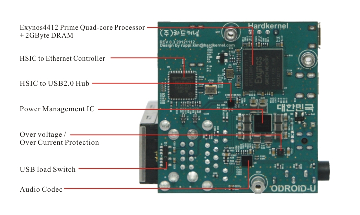
\includegraphics[width=\textwidth]{odroid_u2_top}
\caption{ODROID-U2 Circuit Board Top View \cite{odroid-u2-board-detail}}
\label{odroid-u2-board}
\end{figure}

\begin{figure}[h]
\centering
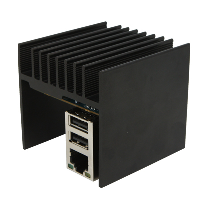
\includegraphics[width=0.25\textwidth]{odroid_u2}
\caption{ODROID-U2 with Heatsink \cite{odroid-u2-board-detail}}
\label{odroid-u2}
\end{figure}

The ODROID-U2 board hosts a Samsung Exynos 4412 Prime System on a Chip
(SoC). \textbf{Figure \ref{odroid-u2-board}} shows the board on its own, and
\textbf{Figure \ref{odroid-u2}} shows the board installed in its heatsink. We
purchased two ODROID-U2 nodes for \$89 each. The board features the following
hardware components \cite{odroid-u2-board-detail}:

\begin{itemize}
\item Samsung Exynos 4412 Prime
  \begin{itemize}
  \item 4 ARM Cortex-A9 cores clocked at 1.7 GHz
  \item 2 GB LPDDR2 RAM
  \end{itemize}
\item SMSC USB3503A USB 2.0 hub
\item SMSC LAN9730 USB 2.0 to 100 Mbps Ethernet controller
\item MAXIM MAX98098 Audio CODEC
\end{itemize}

\begin{figure}[h]
\centering
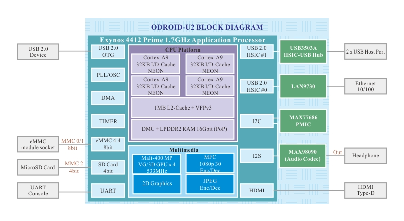
\includegraphics[width=\textwidth]{odroid_u2_block_diagram}
\caption{ODROID-U2 Block Diagram \cite{odroid-u2-board-detail}}
\label{odroid-u2-block-diagram}
\end{figure}

While the ODROID-U2 features impressive raw processing power for its size and
price, its small amount of main memory can adversely impact performance for even
moderately sized parallel simulation models. Additionally, the LAN9730 network
controller is even slower than we feared, routinely reaching end-to-end TCP
small message latency over 500 microseconds.


\subsection{\textbf{ODROID-XU}}

\begin{figure}[h]
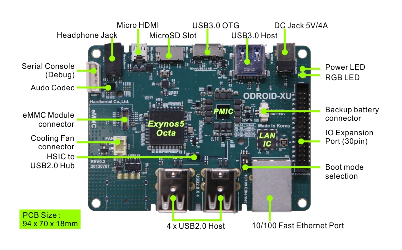
\includegraphics[width=\textwidth]{odroid_xu_top}
\caption{ODROID-XU Circuit Board Top View \cite{odroid-xu-board-detail}}
\label{odroid-xu-board}
\end{figure}

\begin{figure}[h]
\centering
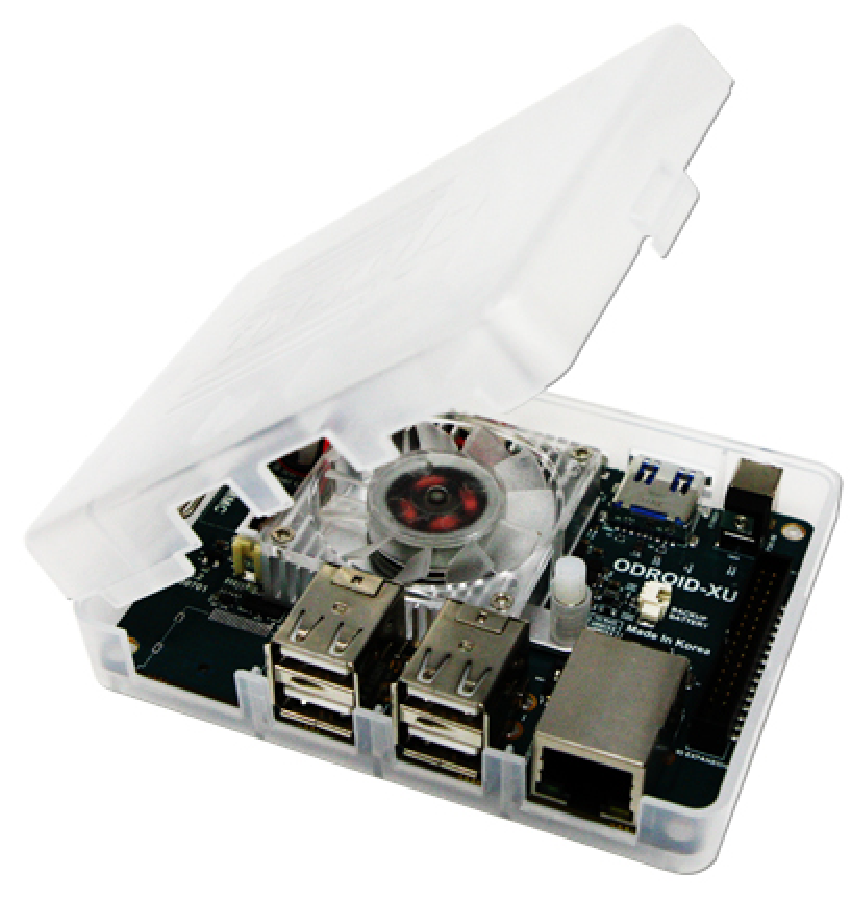
\includegraphics[width=0.5\textwidth]{odroid_xu}
\caption{ODROID-XU Board as Shipped \cite{odroid-xu-board-detail}}
\label{odroid-xu}
\end{figure}

The ODROID-XU features the Samsung Exynos 5410 SoC. We purchased four of these
for \$169 each to form our final four-node cluster. \textbf{Figure
  \ref{odroid-xu-board}} shows the top of the ODROID-XU circuit board without
the processor heatsink and fan installed. \textbf{Figure \ref{odroid-xu}} shows
the ODROID-XU in its plastic case. Clearly, the ODROID-XU has a lower physical
profile than the ODROID-U2 because its heatsink is smaller. However, in terms of
the circuit boards alone, the ODROID-XU is larger than the ODROID-U2. Because
the ODROID-XU has the same network controller as the ODROID-U2, we also
purchased four USB 3.0 to Gigabit Ethernet modules that reduce end-to-end TCP
small message latency to under 300 microseconds. Further details on the
ODROID-XU follow \cite{odroid-xu-board-detail}. Note that the USB 3.0 controller
is not specified on the Hardkernel website.

\begin{itemize}
\item Samsung Exynos 5410 Octa
  \begin{itemize}
  \item 4 ARM Cortex-A15 cores with DVFS support
  \item 4 ARM Cortex-A7 cores
  \item 2 GB LPDDR3 RAM
  \end{itemize}
\item SMSC USB3503A USB 2.0 hub
\item SMSC LAN9730 USB 2.0 to 100 Mbps Ethernet controller
\item MAXIM MAX98098 Audio CODEC
\item ASIX AX88179 USB3.0 to Gigabit Ethernet Controller
\end{itemize}

\begin{figure}[h]
\centering
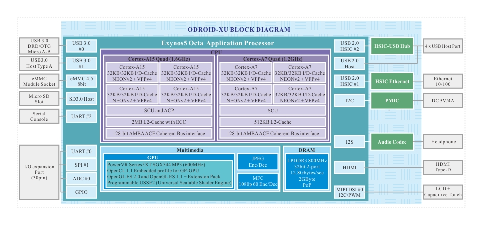
\includegraphics[width=\textwidth]{odroid_xu_block_diagram}
\caption{ODROID-XU Block Diagram \cite{odroid-xu-board-detail}}
\label{odroid-xu-block-diagram}
\end{figure}


The eight processor cores on the ODROID-XU's SoC are arranged in a big.LITTLE
configuration. This heterogeneous computing platform presents some interesting
opportunities specific to this hardware. For example, it would be advantageous
to bind a polling network driver for execution on one of the ``little''
Cortex-A7 cores, leaving all four of the ``big'' Cortex-A15 cores available for
computing work. It might also be possible to dedicate one or more of the
Cortex-A7 cores to overhead tasks in parallel simulation, again allowing for
more of the Cortex-A15 group's raw processing power to be used for parallel
simulation.

Unfortunately, the only supported operating mode for the ODROID-XU is currently
``cluster migration.'' That is, either all four ``little'' cores are active, or
all four ``big'' cores are active. Development of a solution that will allow all
eight cores to run simultaneously is ongoing at Hardkernel.

\section{\textbf{Related Work}}



Although performance profiling of hardware IB and RoCE is extensive
\cite{subamaroni-09} \cite{vienne-12}, studies on software RoCE are
rare. Robert J. Lancaster \cite{lancaster-10} experimented with the \verb;rxe;
driver. He found that \verb;rxe; message latency ranged from 14\% to 81\% lower
than TCP/IP using a Realtek 8168B Gigabit Ethernet adaptor with the r8169
driver.

Trivedi et al. \cite{trivedi-11} experimented with a software implementation of
iWARP for use in cloud computing. They found that end-to-end latencies were
reduced for messages larger than 64 kB thanks the protocol's lightweight RDMA
implementation.

Rajovic et al. \cite{rajovic-13} examined some mobile SoC platforms in order to
evaluate their usefulness for HPC applications. They used the Open-MX
interconnect to reduce network latency in these tests, and elected to use the
NVIDIA Tegra 2 platform to build and deploy a large-scale cluster
\cite{rajovic-14}. They focused on scientific computing and other coarse-grained
parallel applications in performance testing, but found that the cluster scales
well for such purposes using a Gigabit Ethernet interconnect.

\newpage
\chapter{Methods for Reducing Network Latency}
\label{latency_reduction}

\section{\textbf{Software RoCE}}

Currently, there is only one open-source software RoCE project: the \verb;rxe;
linux driver. Previous work in our laboratory has proven that it is capable of
providing significant reduction in network latency when used in an x86 machine
\cite{lancaster-10}.

System Fabric Works created the driver with at least two goals in mind: to
provide a low-cost gateway to InfiniBand software and to function as a testbed
for IB application development \cite{pearson-10}. In both cases, its lack of
network hardware dependence distinguishes it from all other InfiniBand transport
implementations. We hoped to leverage this technology for use in our low-cost
cluster in order to bring its PDES performance closer to the performance of a
traditional x86 cluster.

\begin{figure}[h]
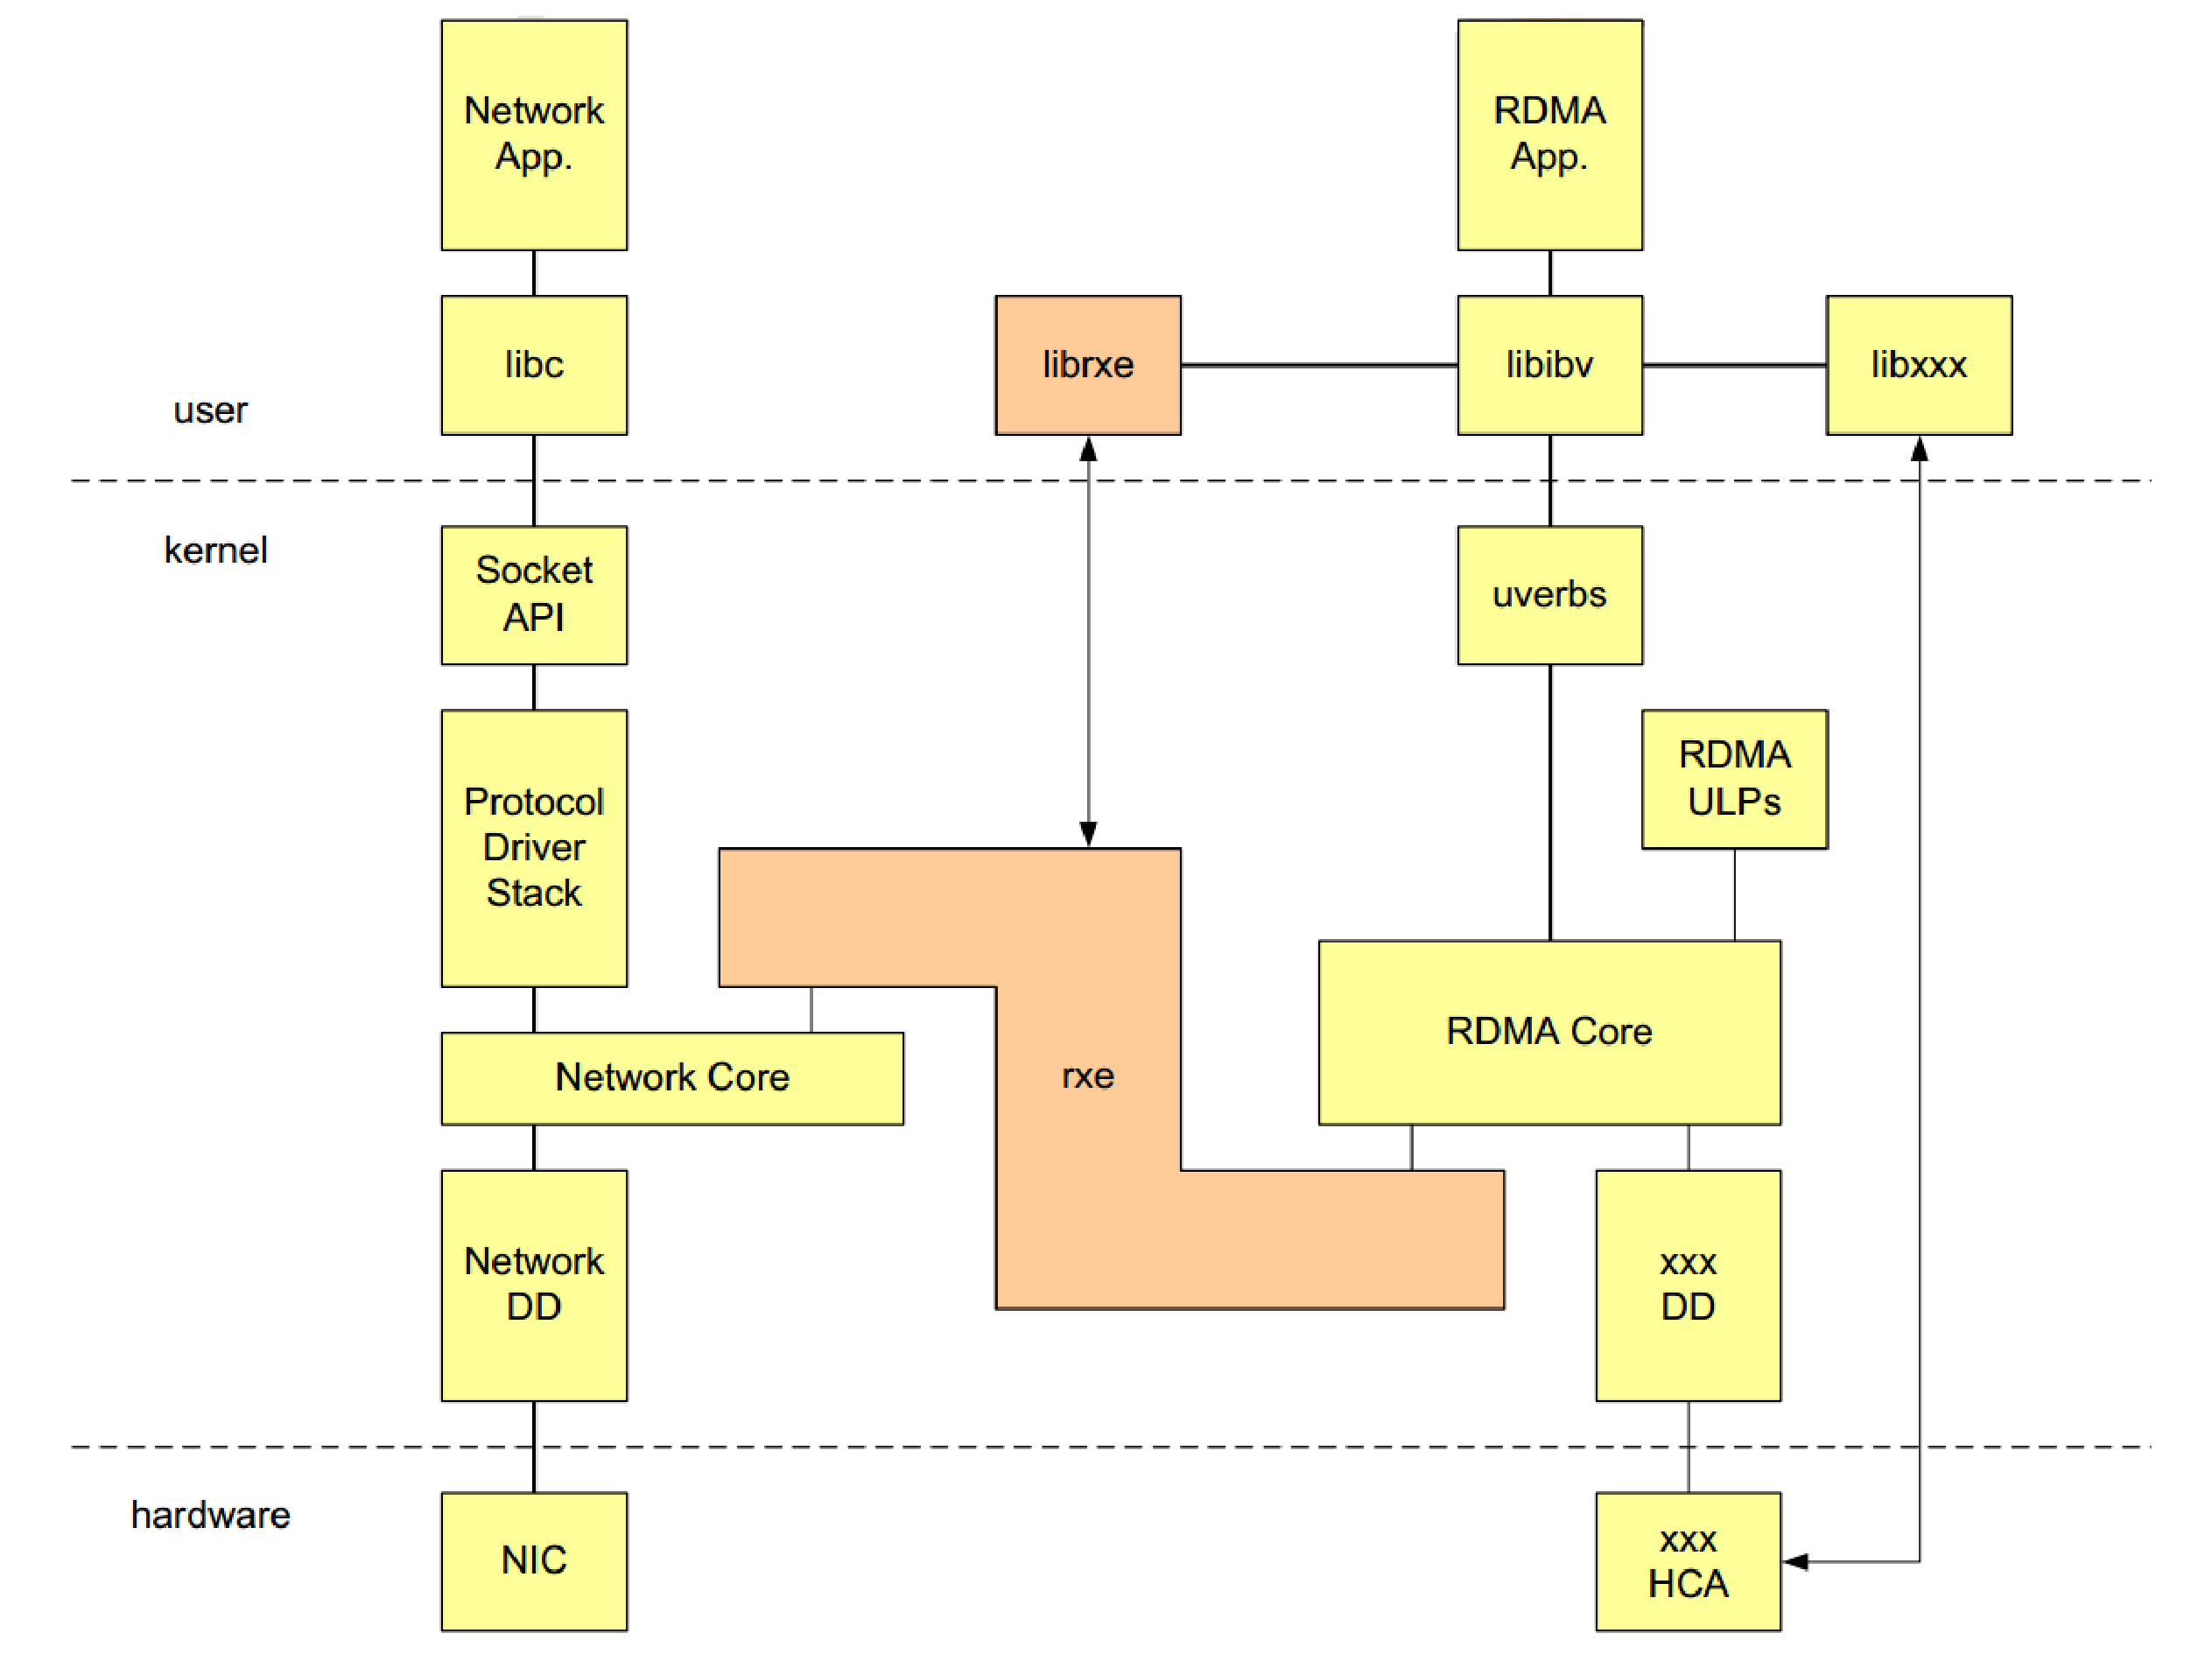
\includegraphics[width=\textwidth]{rxe_linux}
\caption{rxe Driver Role in a Linux Networking Environment \cite{pearson-10}}
\label{rxe-linux}
\end{figure}

\textbf{Figure \ref{rxe-linux}} illustrates how the \verb;rxe; driver functions
as a bridge between RDMA software and the Linux networking core.

The \verb;rxe; linux driver is divided into two modules: \verb;rxe; and
\verb;rxe-net; \cite{pearson-10}. \verb;rxe; provides an implementation of the
InfiniBand transport compliant with the RoCE specification annex
\cite{InfiniBandTARoCE-10}. \verb;rxe-net; interfaces with the Linux networking
stack to transmit and receive packets earmarked for \verb;rxe;
\cite{pearson-10}. The following two sections detail the design of these
modules.

The \verb;rxe; driver also interfaces with a user-mode library called
\verb;librxe;. This library provides the common InfiniBand verbs
interface so that any compliant IB application can use the \verb;rxe; device
without any modification. This library is essentially a user-mode wrapper for
 the functions found in the rxe driver, so its design will not be detailed here.

\subsection{\textbf{rxe}}
\label{rxe}

The \verb;rxe; kernel module contains the portion of the \verb;rxe; driver that
implements layers 4 through 7 of the OSI model. It provides a software
implementation of the InfiniBand RoCE transport. As with all IB
verbs applications, memory is preallocated in Memory Regions (MR), and coupled
pairs of send and receive queues called ``queue pairs'' (QPs) are allocated by
the application based on its needs. That is, QPs are configurable at allocation
time in terms of both queue depth and entry length
\cite{InfiniBandTARoCE-10}\cite{InfiniBandTABase-07}. QPs can be resized after
they are created, but such an operation may adversely impact performance
\cite{InfiniBandTARoCE-10}.

\begin{figure}[h]
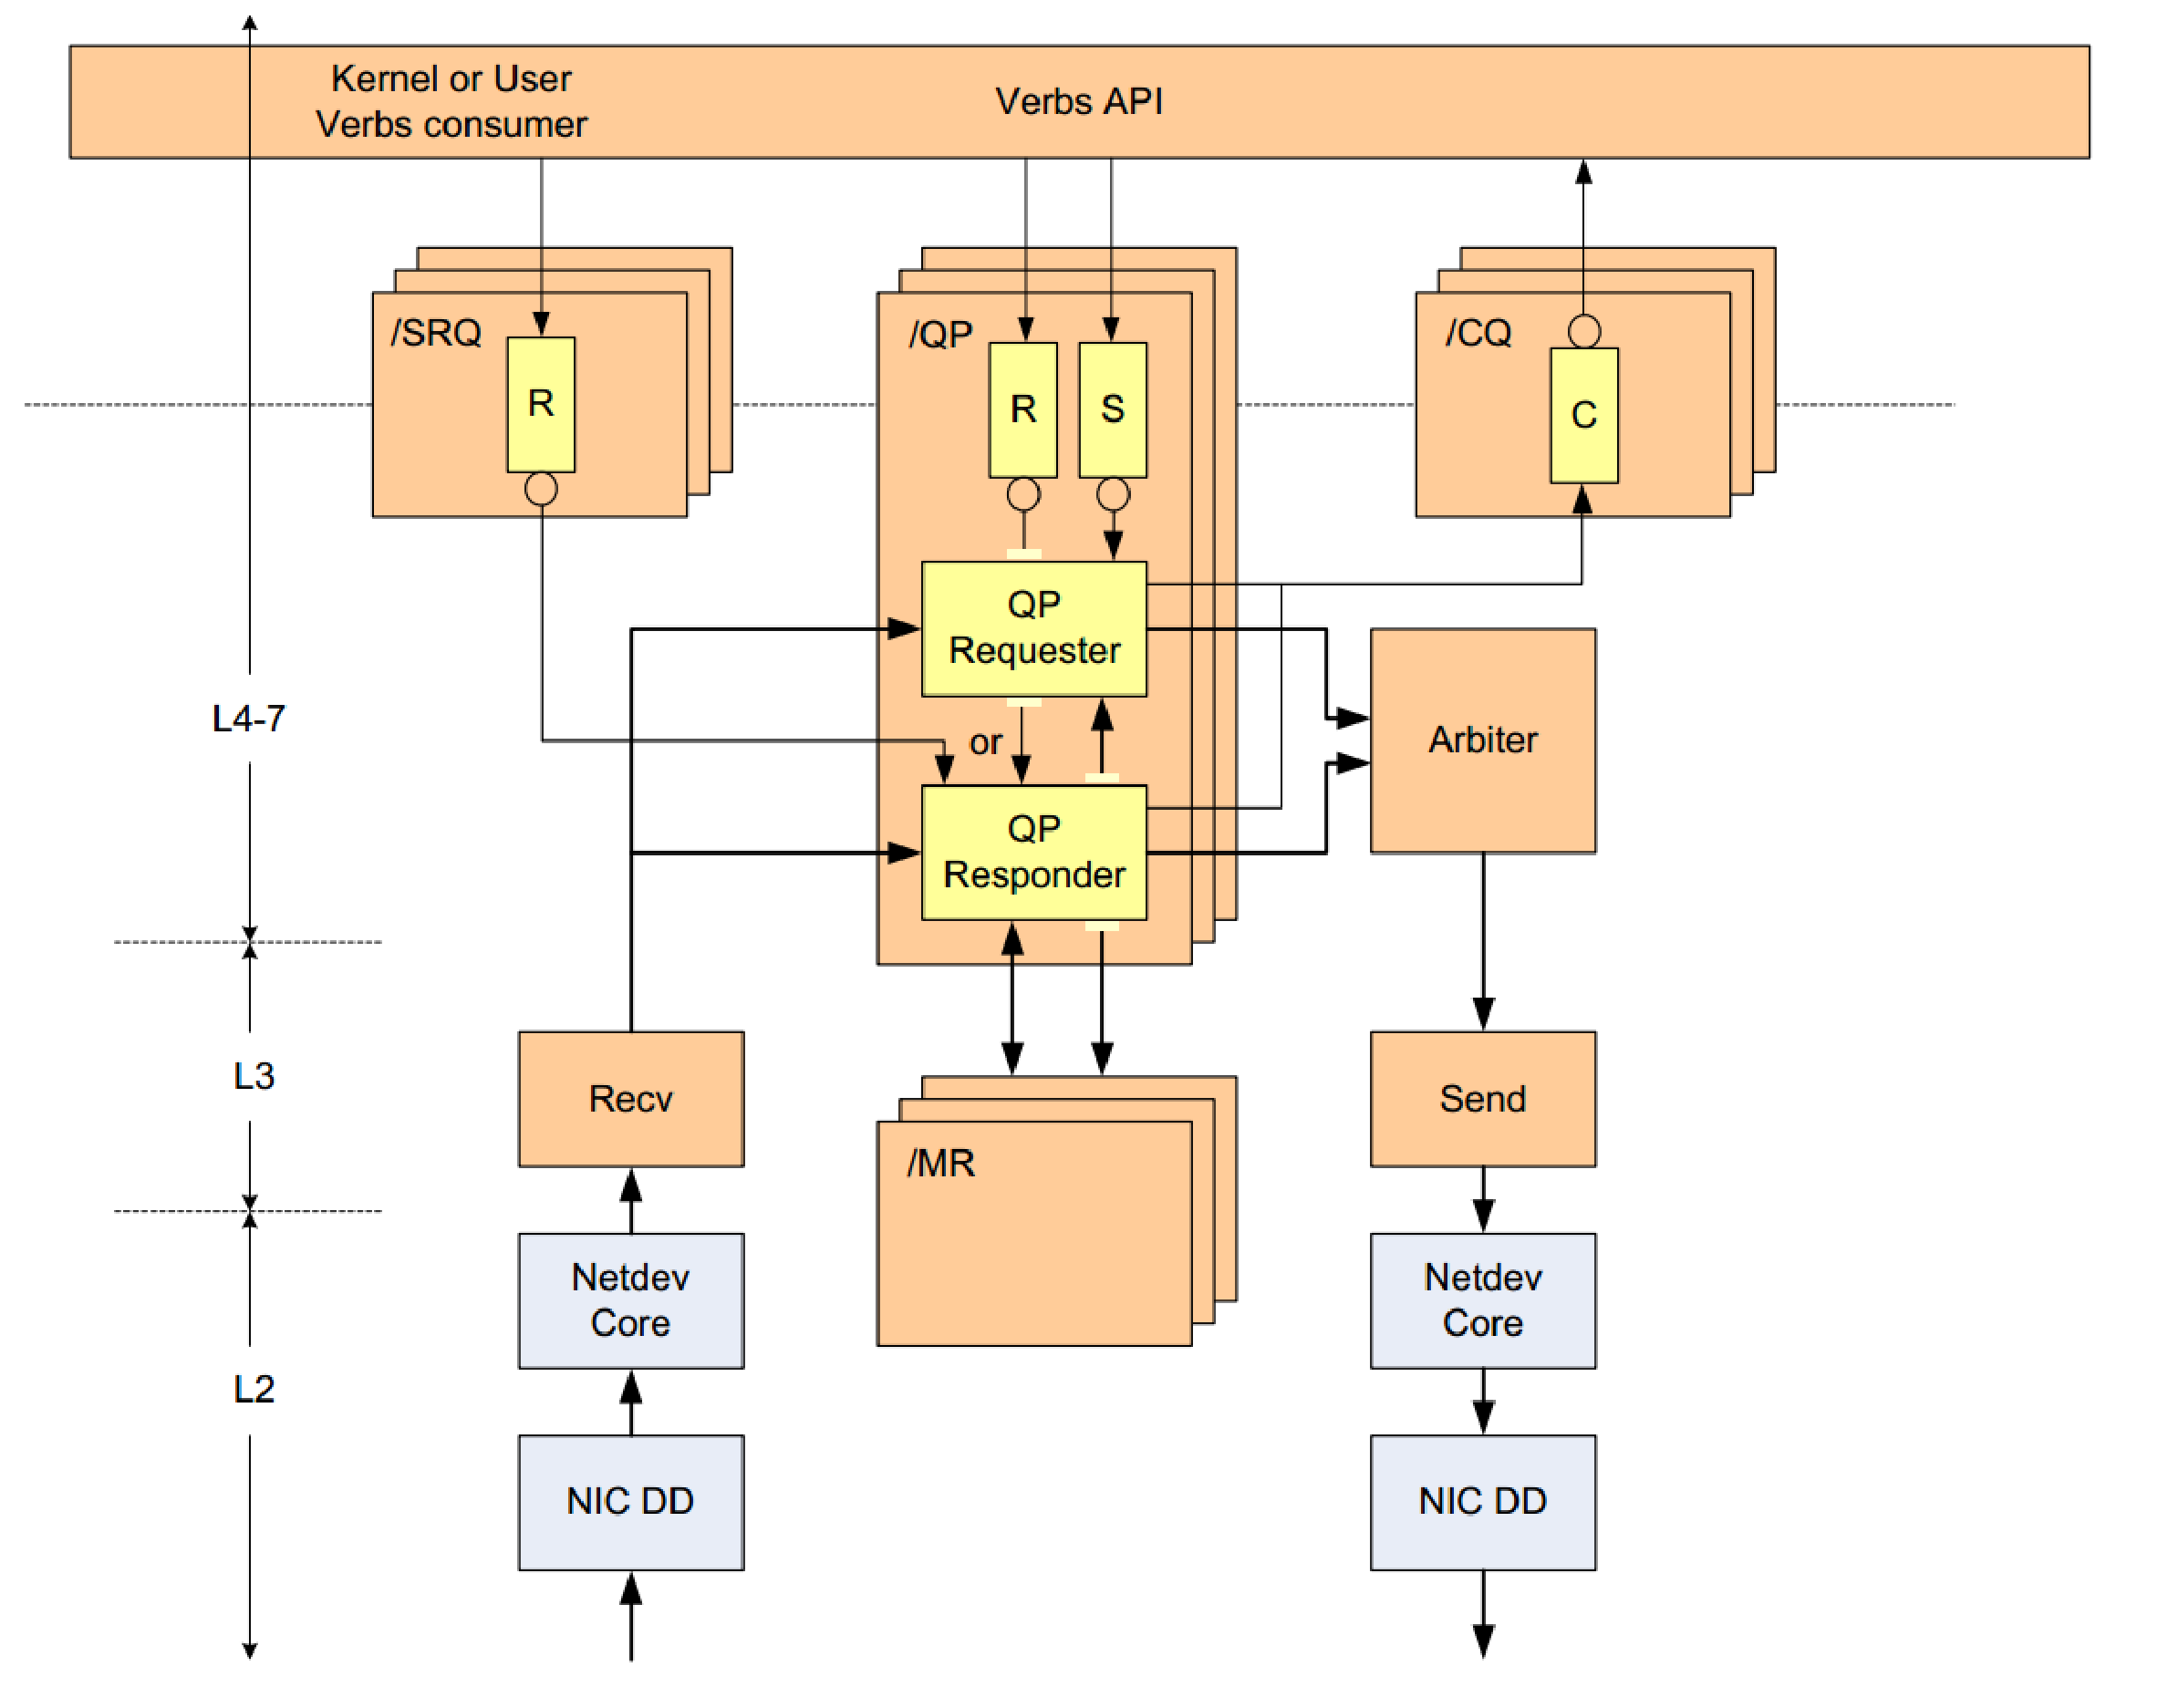
\includegraphics[width=\textwidth]{rxe_overview}
\caption{rxe Driver Overview \protect\cite{pearson-10}}
\label{rxe-overview}
\end{figure}

\textbf{Figure \ref{rxe-overview}} shows the dataflow among the major partitions
of the rxe driver. When a consumer application intends to send or receive a
message, it must submit a Work Request (WR) via an IB verbs function call. This
function places the WR into a QP allocated for that application. If the
application uses Shared Receive Queue (SRQ) semantics (as OpenMPI does), then
another small wrinkle is added for receive WRs as both the SRQ and the QP
associated with the WR must be resolved. Once the Linux kernel is notified that
a WR has been enqueued, the QP Requester and QP Responder routines work to
complete that request. When a WR has been completed, an entry is placed in a
Completion Queue (CQ) that can be accessed by the verbs application. This
Completion Queue Entry (CQE) contains information that the application needs in
order to consider the WR completed.

\begin{figure}[h]
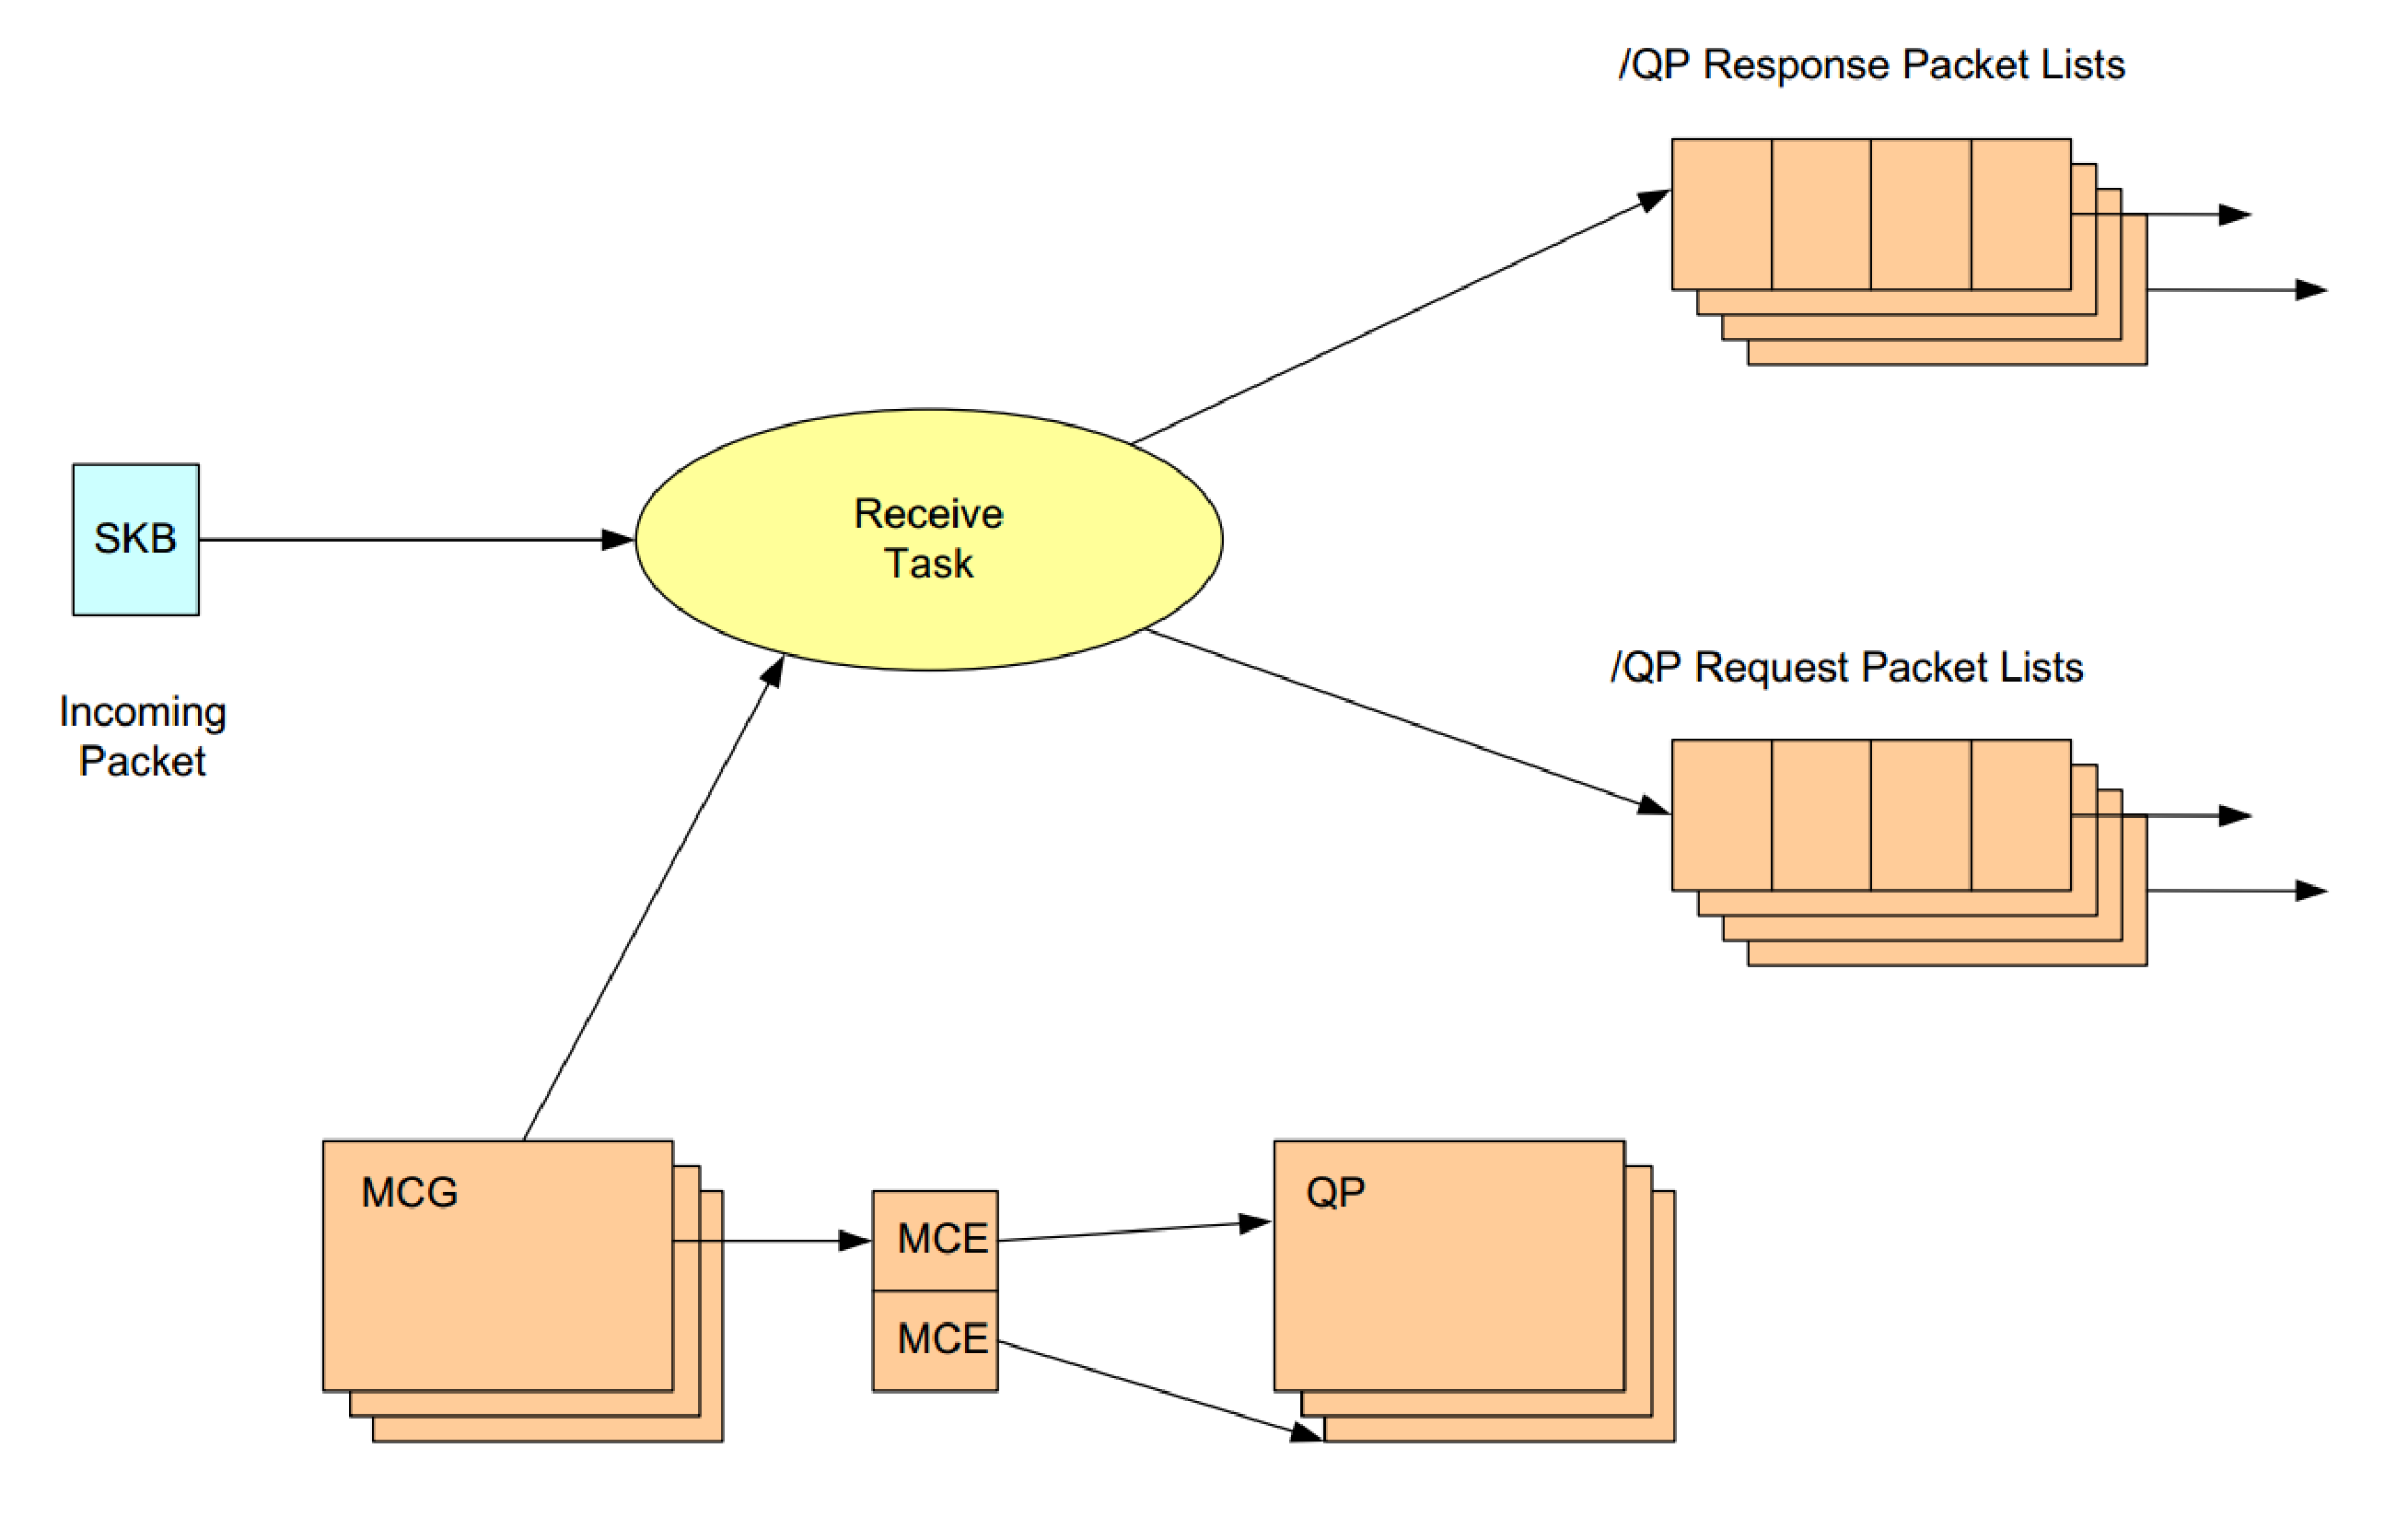
\includegraphics[width=\textwidth]{rxe_recv}
\caption{rxe Receive Task \protect\cite{pearson-10}}
\label{rxe-recv}
\end{figure}

The Layer 4 portion of the \verb;rxe; driver's Receive routine is illustrated in
\textbf{Figure \ref{rxe-recv}}. This function receives a socket buffer (SKB)
from \verb;rxe-net; as an input. It inspects the SKB header in order to
determine whether the message is a response packet or a request packet and
places the SKB into a corresponding packet list in the receive queue.

\begin{figure}[h]
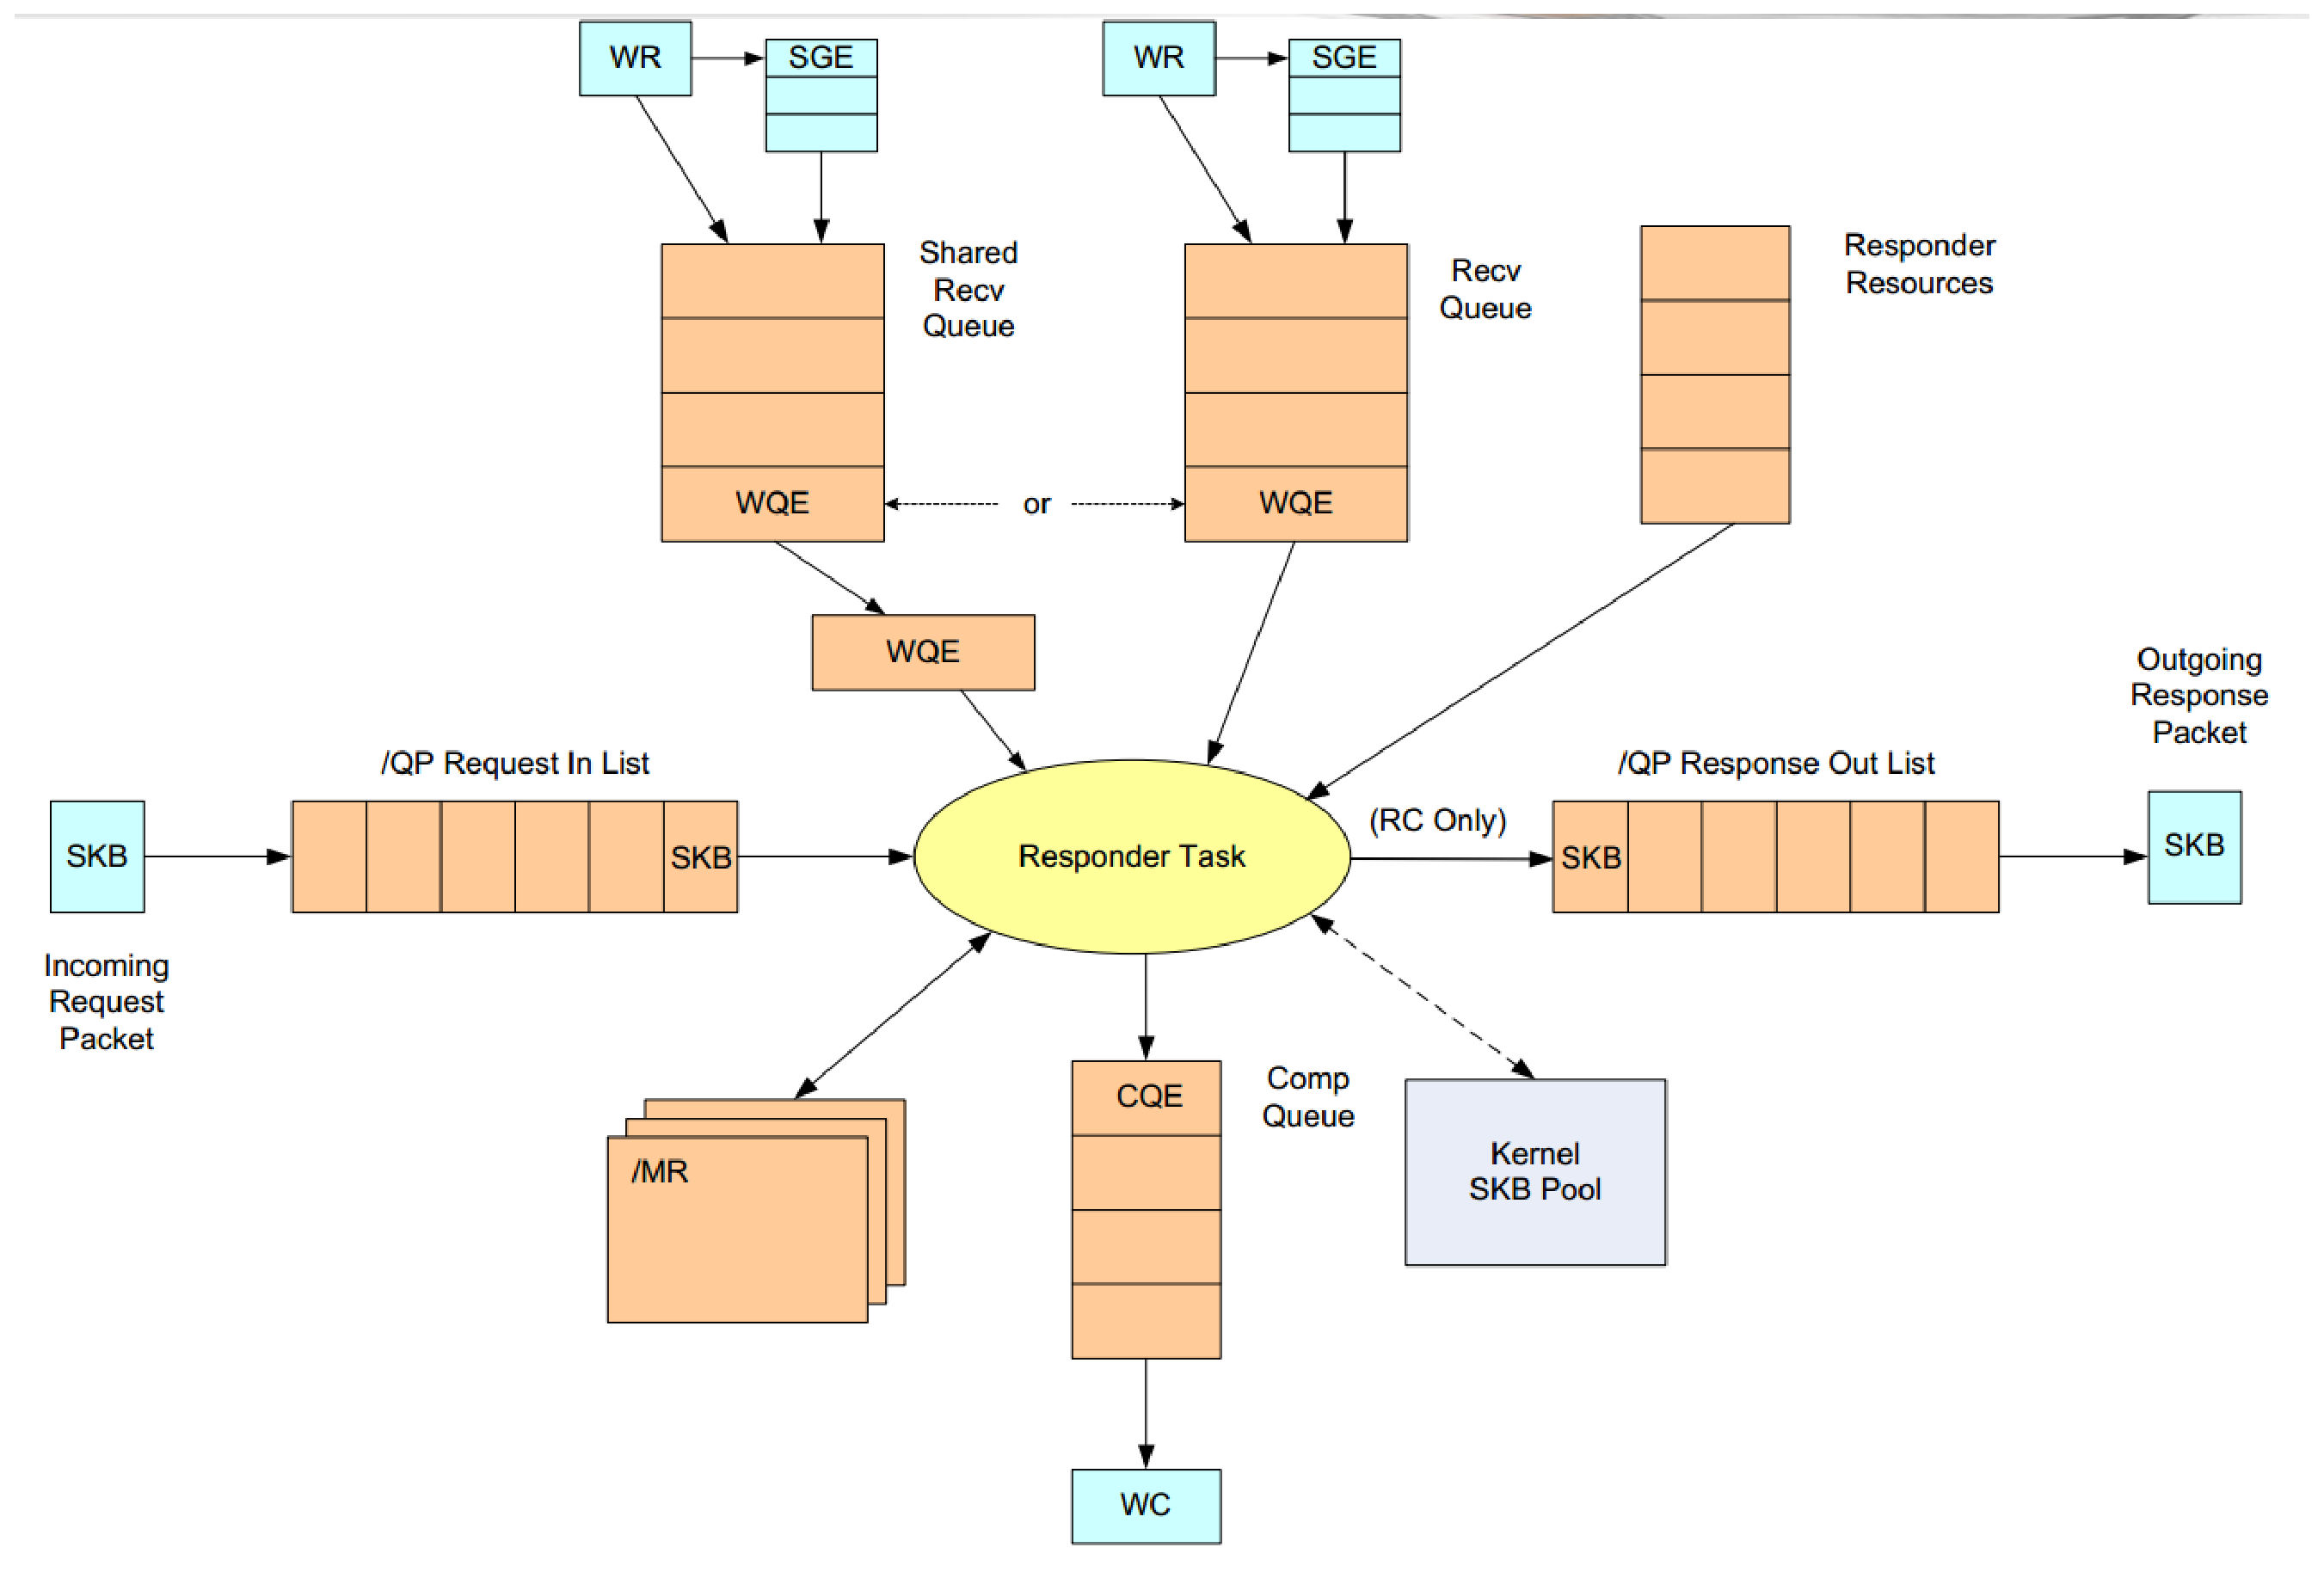
\includegraphics[width=\textwidth]{rxe_resp}
\caption{rxe QP Responder Architecture \protect\cite{pearson-10}}
\label{rxe-resp}
\end{figure}

The QP Responder's architecture is illustrated in \textbf{Figure
  \ref{rxe-resp}}. The Responder partition contains functions that respond to
incoming requests for data. Such a request can be in one of two forms: a socket
buffer (SKB) sent from \verb;rxe-net; or a WR from a receive queue. For both
cases, the Responder retrieves the requested data and generates a CQE
\cite{pearson-10}. If the connection associated with the request uses Reliable
Connection (RC) semantics, then a response message is generated and placed in
the send queue \cite{InfiniBandTARoCE-10}\cite{pearson-10}. Additonally, if a
request represents an atomic operation, the responder must save some state in
order to support retries for all message semantics and unordered read/write
operations for RDMA semantics. In \textbf{Figure \ref{rxe-resp}}, this is
represented by the ``Responder Resources'' data structure.

\begin{figure}[h]
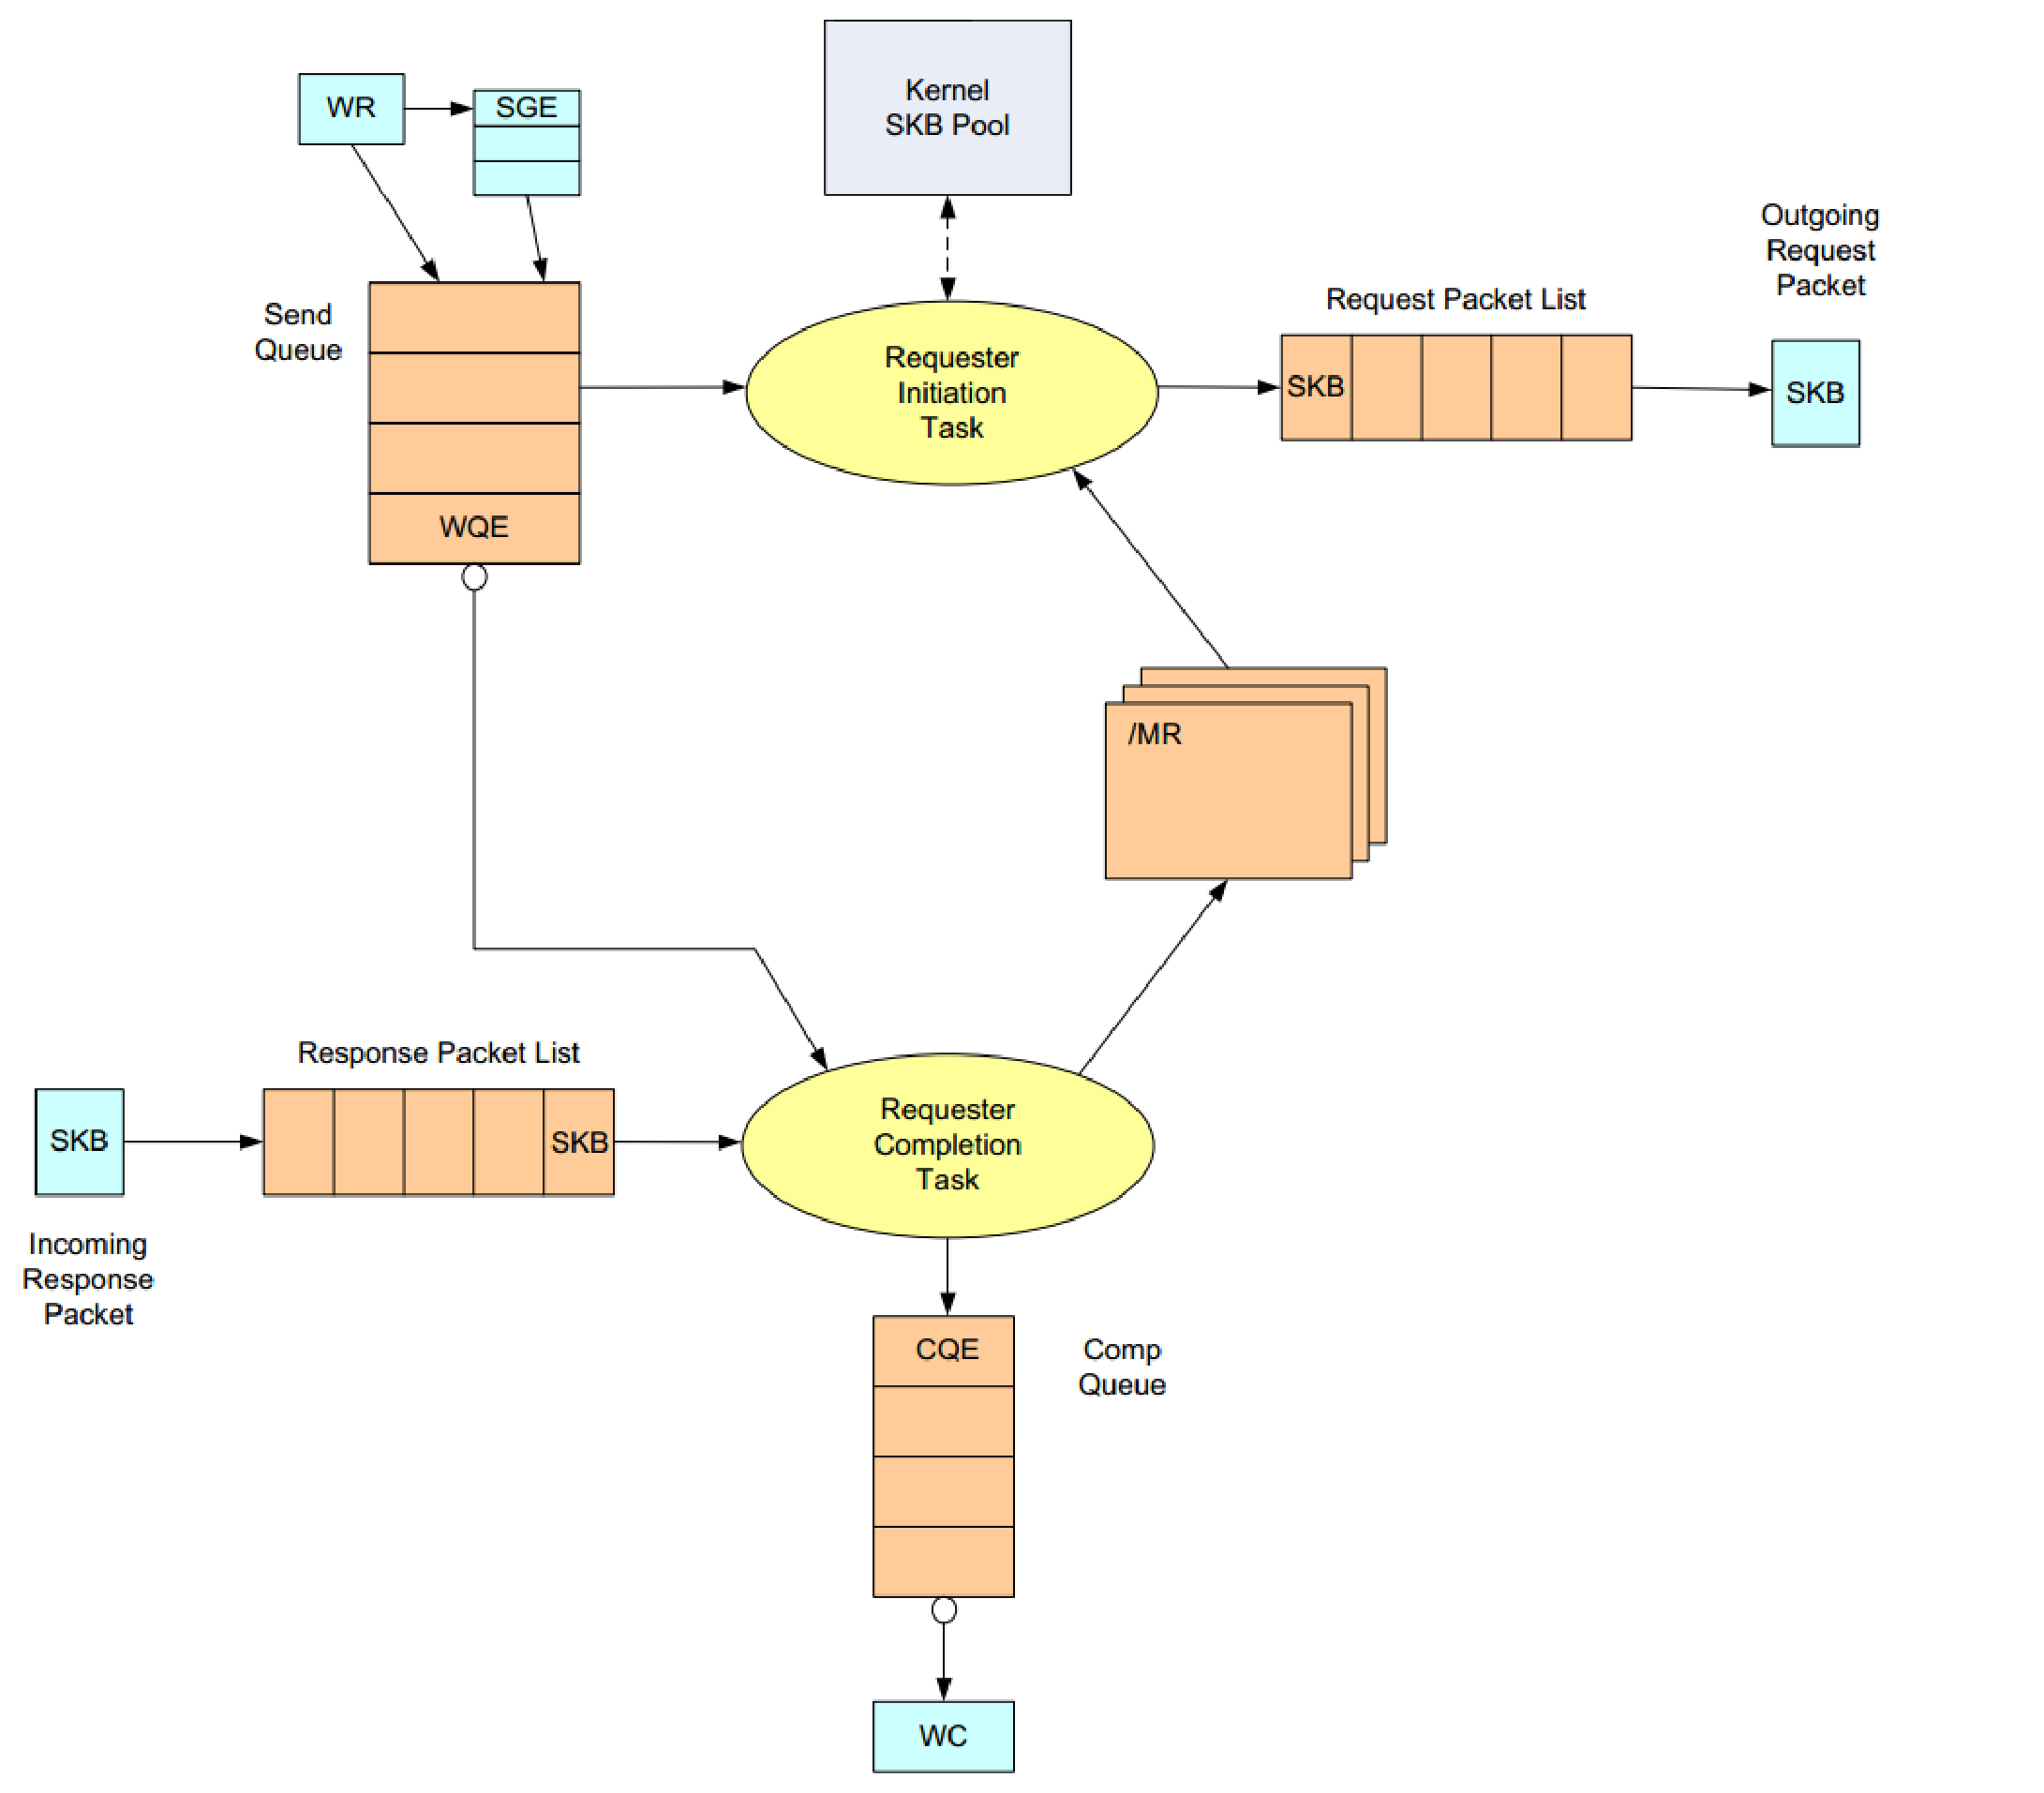
\includegraphics[width=\textwidth]{rxe_req}
\caption{rxe QP Requester Architecure \protect\cite{pearson-10}}
\label{rxe-req}
\end{figure}

The QP Requester's architecture is illustrated in \textbf{Figure
  \ref{rxe-req}}. The Requester is further divided into an Initiator task and a
Completer task. The Initiator simply creates a request message for every entry
in the send queue. The Completer is active only for communication using the
Reliable Connection (RC) channel semantics. It waits for responses from the
remote node to indicate that each WQE has been retired\cite {pearson-10}. It
then generates a CQE and releases the WQE. If a message fails and must be
retried, the Initiator can be reset to the point where the Completer is
waiting. For all other channel sematics, the WQE is retired and released
immediately by the Initiator without invoking the Completer.

\begin{figure}[h]
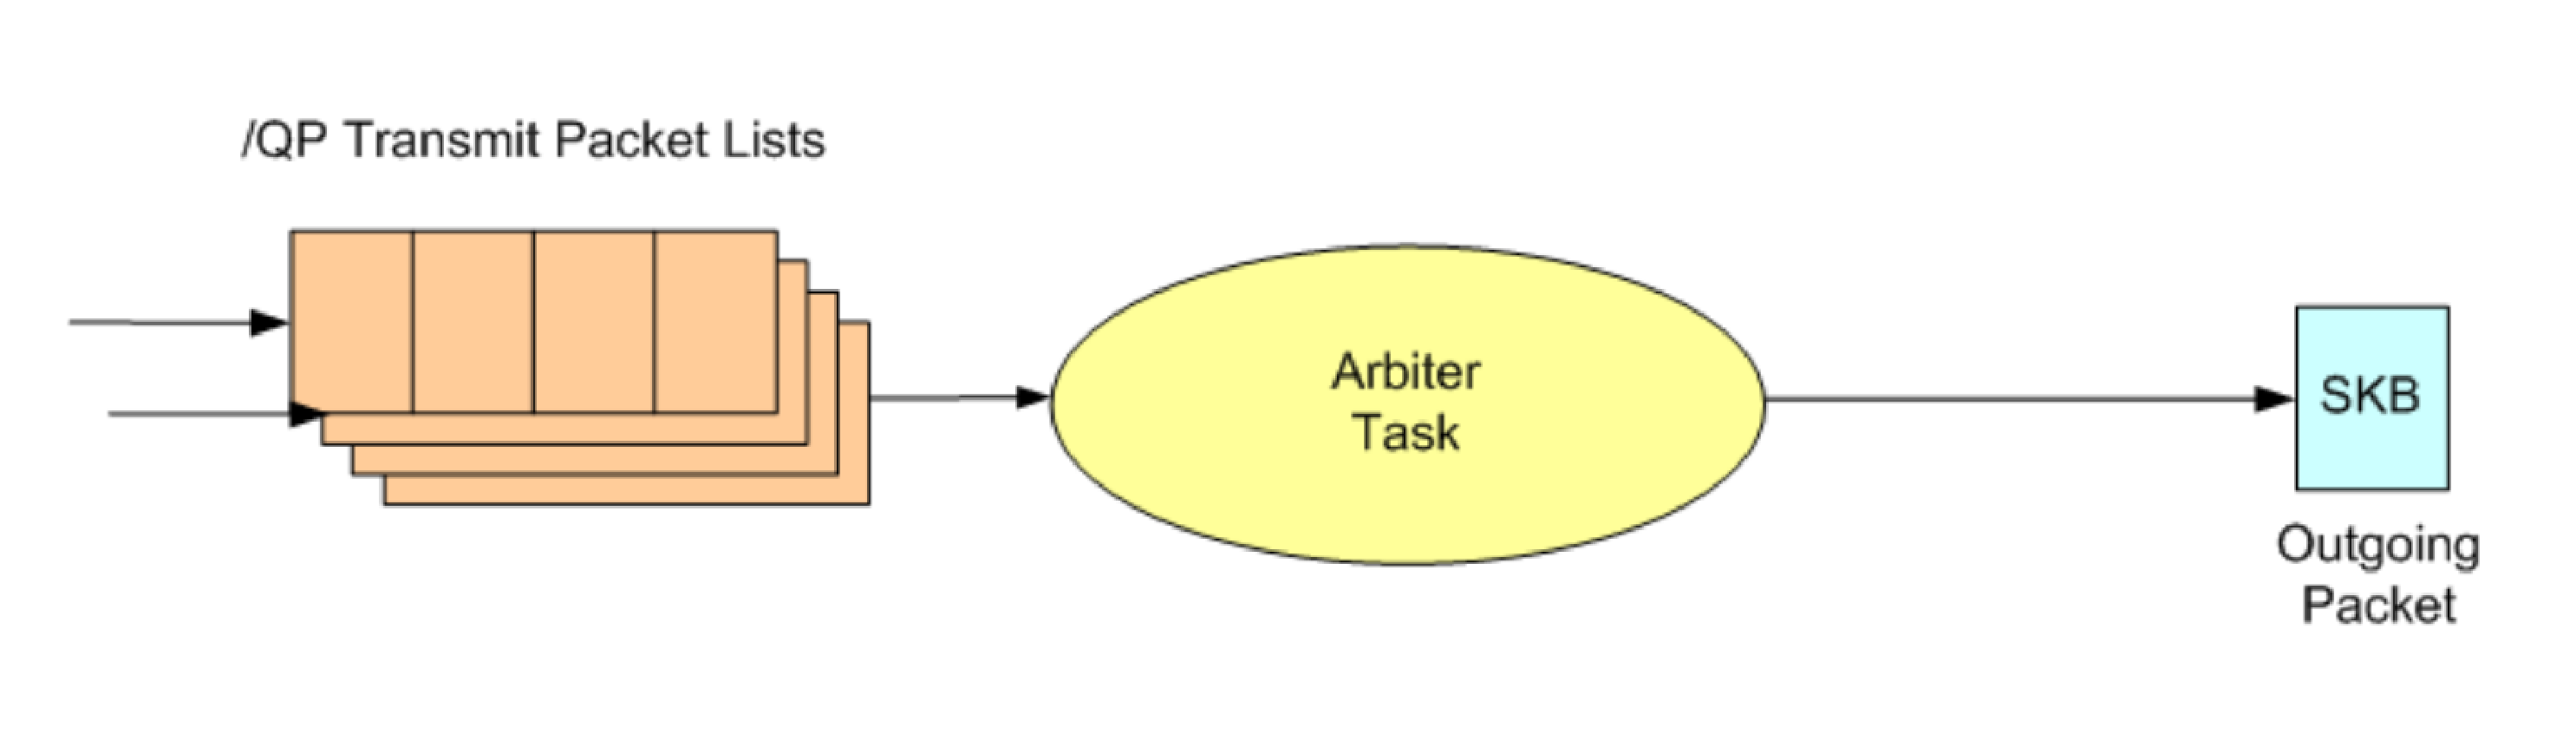
\includegraphics[width=\textwidth]{rxe_arbiter}
\caption{rxe Arbiter Architecture \protect\cite{pearson-10}}
\label{rxe-arbiter}
\end{figure}

The Arbiter task is illustrated in \textbf{Figure \ref{rxe-arbiter}}. It
schedules actual transmission of outgoing messages. It implements a round-robin
scheduling policy among all active send queues, and it also handles flow control
in order to avoid packet dropping in Linux due to queue overrun
\cite{pearson-10}. This flow control includes a static minimum time between
packet transmissions. This parameter and others in the Arbiter can be tuned
while the module is loaded, and the Arbiter can even be disabled
altogether. In our research with the ODROID-U2, lowering or removing these
timing thresholds had no effect on end-to-end latency on a 100 Mbps Ethernet
link.

\subsection{\textbf{rxe-net}}

In many ways, the \verb;rxe-net; module functions as a wrapper for the
\verb;rxe; transport module described in \textbf{Section \ref{rxe}}. It
implements most of layer 3 of RoCE, allowing the layer 4 and higher functions of
\verb;rxe; to integrate with the existing layer 2 networking implementation in
Linux by forming a bridge that communicates with Linux on both the RDMA and
Ethernet sides. It can be envisioned as the horizontal portion of the \verb;rxe;
driver in \textbf{Figure \ref{rxe-linux}}. In addition to facilitating this
communication and marshalling of data, \verb;rxe-net; writes the appropriate
combination of InfiniBand and MAC headers to each packet in order to fulfill the
requirements of the RoCE specification \cite{pearson-10}
\cite{InfiniBandTARoCE-10}. In accordance with the specification, the Ethernet
MAC (layer 2) header is identical to a normal ethernet packet except for the
ethertype value, which is set to \verb;0x8915; for all RoCE packets
\cite{InfiniBandTARoCE-10}. \textbf{Figure \ref{roce-packet}} compares normal
InfiniBand packets to RoCE packets \cite{ayoub-11} \cite{InfiniBandTABase-07}
\cite{InfiniBandTARoCE-10}.

\begin{figure}[h]
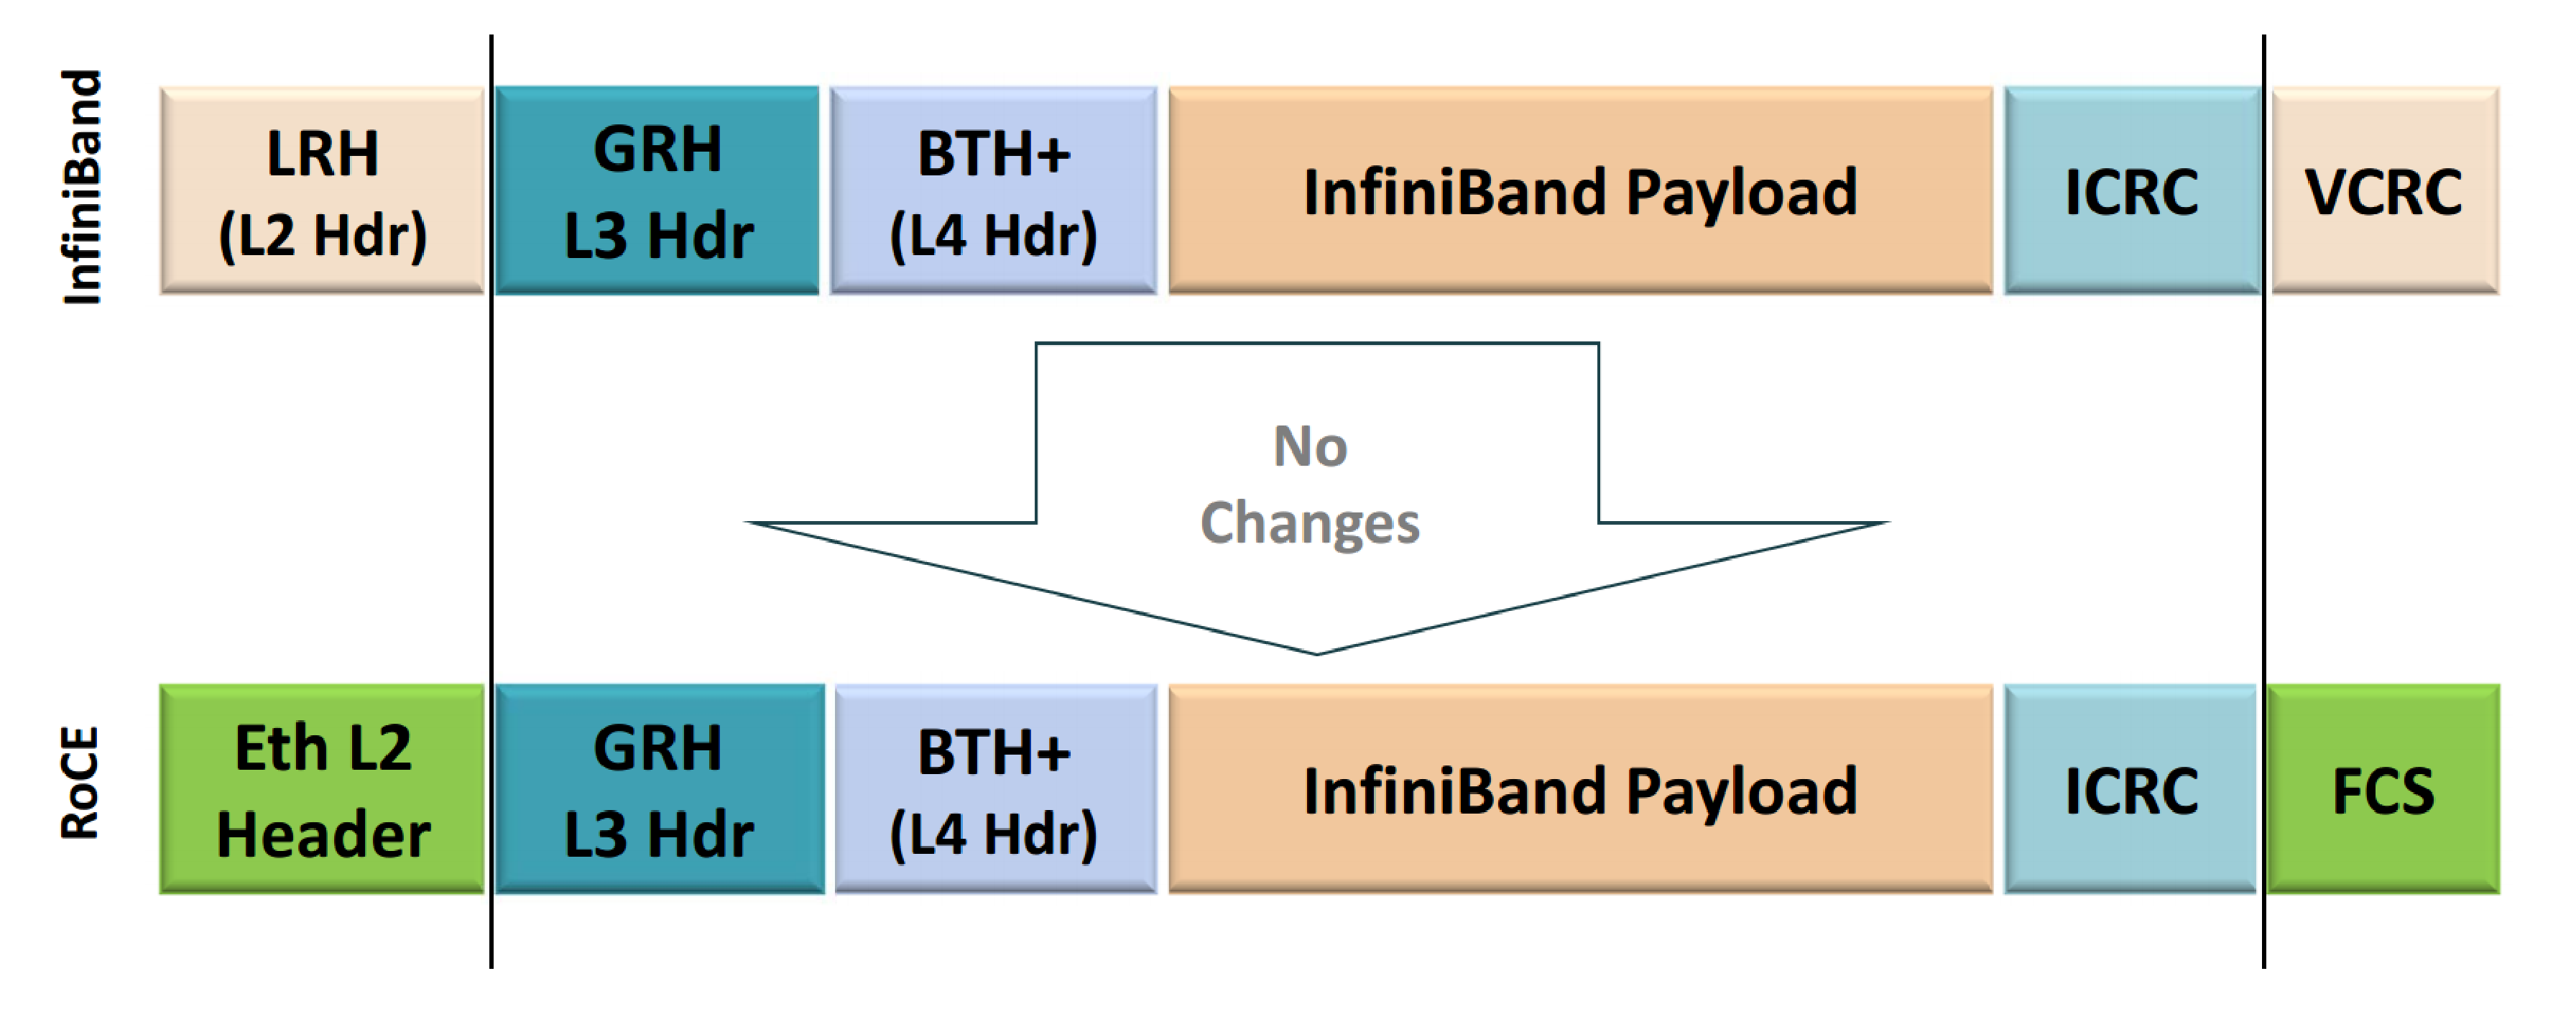
\includegraphics[width=\textwidth]{roce_packet}
\caption{RoCE Packet Composition \cite{ayoub-11}}
\label{roce-packet}
\end{figure}

\subsection{\textbf{Porting rxe to the ODROID Platform}}

Although \verb;rxe; is designed to operate with any Ethernet adaptor, it also
depends on the IB libraries in the Linux kernel. These libraries, in turn,
depend on the presence of a PCI bus in the host system. Neither the ODROID-U2
nor the ODROID-XU has PCI support. Simply enabling PCI support in the Linux
kernel configuration creates some incompatibilites that must be resolved before
the kernel will work correctly. After some trial and error, I found a solution:
the addition of the line in \textbf{Figure \ref{pci_code}} near the beginning of
\verb;drivers/pci/probe.c;.

\begin{figure}[h]
\centering
\begin{verbatim}
#define pcibios_assign_all_busses() 1
\end{verbatim}
\caption{Code Added to drivers/pci/probe.c}
\label{pci_code}
\end{figure}

The most significant porting effort involved updating the \verb;rxe; driver to
work correctly with the ARM linux memory model. ARM Linux has several subtle
differences from x86 Linux in the way the kernel maps memory. This resulted in
some incompatibilities with the rxe code. Chiefly, the rxe code does not support
the mapping of high memory (userspace memory) into low memory (kernel memory) at
runtime. This is an important feature in modern IB drivers because it allows
memory regions to be directly accessed by userspace programs, eliminating some
need for high-latency context switches. \verb;rxe; currently uses the
\verb;page_address(); macro to get virtual page addresses. These calls should be
replaced by \verb;kmap(); or \verb;kmap_atomic(); in order to make them safe for
use on high memory pages. However, each \verb;kmap(); call requires a
corresponding \verb;kunmap();. Some of the \verb;rxe; DMA memory mapping
functions use the \verb;page_address(); macro to return an address for DMA
operations. This is not an intended use for \verb;kmap();, because the kernel
has a limited number of such mappings available. It is also difficult to change,
because the \verb;page_address(); macro does not require an unmap call, while
\verb;kmap(); requires a matching \verb;kunmap(); call. We were able to run the
driver recoded with \verb;kmap(); calls for use with micro-benchmarks, but it is
unstable when used with MPI applications. We concluded that a major overhaul of
the \verb;rxe; DMA architecture would be required to support high memory on the
driver side.

Luckily, this problem is easily resolved by configuring the kernel to map all
memory to a single region, eliminating the distinction between user and kernel
address space. The ODROID-U2 and ODROID-XU only have 2046 MB of main memory, so
a 32-bit processor can map it all into a single address space. However, the
\verb;vmalloc; virtual memory region can overlap with some of this space,
causing the Linux kernel to ignore or truncate regions of address space that
should be mapped to physical memory. This limitation can be partially bypassed
by reconfiguring the size of the \verb;vmalloc; region using Linux kernel
parameters \cite{vmalloc-overlap}. Additionally, it is possible to move the
region by altering the values of the \verb;VMALLOC_START; and \verb;VMALLOC_END;
macros, then shifting the \verb;IO_ADDRESS; macro accordingly so memory-mapped
I/O devices still have their own address space. For the ODROID-XU, this process
enabled the use of 1884 MB of memory, while the remaining 163 MB were dedicated
to I/O devices. The final address space mapping is shown in \textbf{Figure
  \ref{addrmap}}.

%% The migration from the ODROID-U2 to the ODROID-XU presented some additional
%% challenges in the porting effort for the rxe driver. I encountered a bug that
%% disrupted the marshalling of Work Requests from userspace to kernel space. This
%% bug was a symptom of TODO. This problem can be solved by TODO.

\begin{figure}[h]
\begin{center}
\begin{verbatim}
Memory: 2046MB = 2046MB total
Memory: 1927936k/1927936k available, 167168k reserved, 0K highmem
Virtual kernel memory layout:
    vector  : 0xffff0000 - 0xffff1000   (   4 kB)
    fixmap  : 0xfff00000 - 0xfffe0000   ( 896 kB)
    vmalloc : 0xc0000000 - 0xff000000   (1008 MB)
    lowmem  : 0x40000000 - 0xbfe00000   (2046 MB)
    modules : 0x3f000000 - 0x40000000   (  16 MB)
      .text : 0x40008000 - 0x409ce000   (10008 kB)
      .init : 0x409ce000 - 0x40a0dfc0   ( 256 kB)
      .data : 0x40a0e000 - 0x40ab8a98   ( 683 kB)
       .bss : 0x40ab8abc - 0x40c7d758   (1812 kB)
\end{verbatim}
\end{center}
\caption{Address Space Mapped by Linux Kernel}
\label{addrmap}
\end{figure}

\section{\textbf{Polling the Network Adaptor}}

Previous research with network drivers has shown that interrupt latency in a
multi-tasking operating system can be eliminated with a polling network driver
\cite{dovrolis-01}\cite{liu-09}. In fact, the Linux TCP/IP networking stack has
moved to a hybrid of polling and interrupt-based event processing that is
intended to reduce average network latency in high-traffic situations. In
Parallel Discrete Event Simulation on multi-core processors, it may even be
advantageous to give up a processor core to a polling driver in order to
significantly reduce message latency for all packets. The big.LITTLE processor
configurations in products like the ODROID-XU make this prospect especially
enticing when one considers that polling could be handled by one of the
``little'' cores, leaving all the ``big'' cores available for event processing.

Although the ability to symetrically multi-process with both ``big'' and
``little'' cores is not yet present for Linux in the ODROID-XU, we pursued this
goal in the hope that the trade of a ``big'' core for reduced latency would
still be worthwhile. Doug Weber and Zakaria Aldeneh began this study by creating
an EHCI polling driver for use with the standard ODROID-XU network
adaptors. Weber later extended this work to an xHCI polling driver used
with the Gigabit Ethernet adaptors for the ODROID-XU.

\subsection{\textbf{EHCI Polling Driver}}

Initial work with the EHCI Polling Driver by Doug Weber and Zakaria Aldeneh
revealed that it could reduce network message latency over TCP by as much as
35\%. This motivated the creation of a similarly architected polling driver
for use with the USB 3 to Gigabit Ethernet adaptors.

\subsection{\textbf{xHCI Polling Driver}}

The eXtensible Host Controller Interface (xHCI) specification \cite{xhci}
describes a structure called a Transfer Request Block (TRB) that represents a
single transaction between a driver and a USB controller. TRBs are placed on a
data structure called a ``ring,'' which is similar to a circular linked list. We
are particularly interested in the Event Ring, which is used by the host
controller to notify a driver of hardware events, including received data.

The architecture of the xHCI polling driver used in this study is contained
within the \verb;xhci_hcd; Linux kernel module. When loaded, the module performs
its normal function in interrupt mode. In interrupt mode, the controller raises
an interrupt when it places a TRB onto the Event Ring. In response, the
operating system executes the Interrupt Service Routine (ISR) associated with the
interrupt. In turn, the ISR schedules a Deferred Procedure Call (DPC) that
performs the necessary processing to handle all unprocessed TRBs on the Event
Ring. Although this process is very fast, some overhead is incurred by the ISR.

When the \verb;poll_option; module parameter is set to 1, it spawns a kernel
thread that loops forever, checking the Event Ring for new TRBs. In this way,
the driver is able to process incoming events immediately, without waiting for
the context switches associated with an ISR. Naturally, this thread completely
utilizes one CPU core. In this case, we hoped that the mitigation of interrupt
latency can improve PDES performance enough to offset the removal of one event
processing core.

Unfortunately, stability issues with this implementation made it impossible to
sufficiently test its performance with MPI network communication.

\newpage
\chapter{Cluster Implementation and Testing}
\label{cluster}

Three primary testing platforms were used for the experiments presented in this
thesis. OpenMPI is used for all MPI communication. Its transport layer selection
feature is used to isolate either the TCP/IP or RoCE transport for individual
tests.

\section{\textbf{ODROID-U2}}

Preliminary work with RoCE was tested on two ODROID-U2 computers running Debian
7.0-armhf with Linux kernel 3.0.90. The ODROID-U2 nodes are connected to an
unmanaged Gigabit switch through Category 6 Ethernet cables. Unless specified
otherwise, the Linux network MTU is set to 1488 bytes and the RoCE MTU is set to
1024 bytes.

\section{\textbf{ODROID-XU}}

The success of RoCE and EHCI polling experiments motivated the purchase of four
ODROID-XU nodes as well as Gigabit Ethernet adaptors for all four nodes. All
tests in theis section are run on four ODROID-XU computers running Debian
8.0-armhf with Linux kernel 3.4.76. The Linux network MTU is set to 1500 bytes,
and the RoCE MTU is set to 1024 bytes.

The total cost of the computing hardware for this cluster is calculated in
\textbf{Table \ref{xu-cost-table}}.

\begin{table}
  \caption{Hardware Cost of ODROID-XU Cluster}
  \label{xu-cost-table}
  \centering
  \begin{tabular}{| l | r |}
    \hline
    \textbf{Component} & \textbf{Cost} \\ \hline
    ODROID-XU board $\times$ 4 & \$169.00 $\times$ 4 \\
    ASIX GbE Adaptor $\times$ 4 & \$25.00 $\times$ 4 \\
    16 GB Class 10 MicroSD card, various vendors $\times$ 4 & \$10.99 $\times$ 4 \\
    Netgear GS108 GbE switch & \$45.99 \\
    \hline
    \textbf{Total} & \textbf{\$865.95} \\ \hline
  \end{tabular}
\end{table}

\section{\textbf{Comparison Cluster}}

We will compare the performance of the ODROID-XU cluster with a small
traditional Beowulf cluster consisting of two x86 PCs running Intel Haswell CPUs
and 32 GB of main memory. Although not all of the hardware components were
purchased specifically for this cluster, the hardware costs of these PCs are
estimated in \textbf{Table \ref{x86-cost-table}}.

\begin{table}
  \caption{Hardware Cost of x86 Cluster}
  \label{x86-cost-table}
  \centering
  \begin{tabular}{| l | r |}
    \hline
    \textbf{Component} & \textbf{Cost} \\
    \hline
    Intel Core i7-4770 CPU $\times$ 2 & \$309.00 $\times$ 2 \\
    32 GB RAM (2 DIMMs) $\times$ 2 & \$318.09 $\times$ 2 \\
    Lynx Point based motherboard $\times$ 2 & \$105.00 $\times$ 2 \\
    Hard Drives & \$150 \\
    Enclosure $\times$ 2 & \$100 $\times$ 2 \\
    Netgear GS108 GbE switch & \$45.99 \\
    \hline
    \textbf{Total} & \textbf{\$1860.17} \\ \hline
  \end{tabular}
\end{table}

Although each Intel processor has only four processor cores, it supports
Simultaneous Multithreading (SMT), presenting eight logical cores to the
operating system. Therefore, two of these x86 nodes will provide the same number
of independent hardware threads as the four ARM nodes.

\section{\textbf{Initial Cost Comparisons}}

The Linux \verb;sysbench; benchmark is used to compare CPU mathematics and
memory performance in order to compare the raw processing power available to
applications running on each cluster.

\begin{figure}
\centering
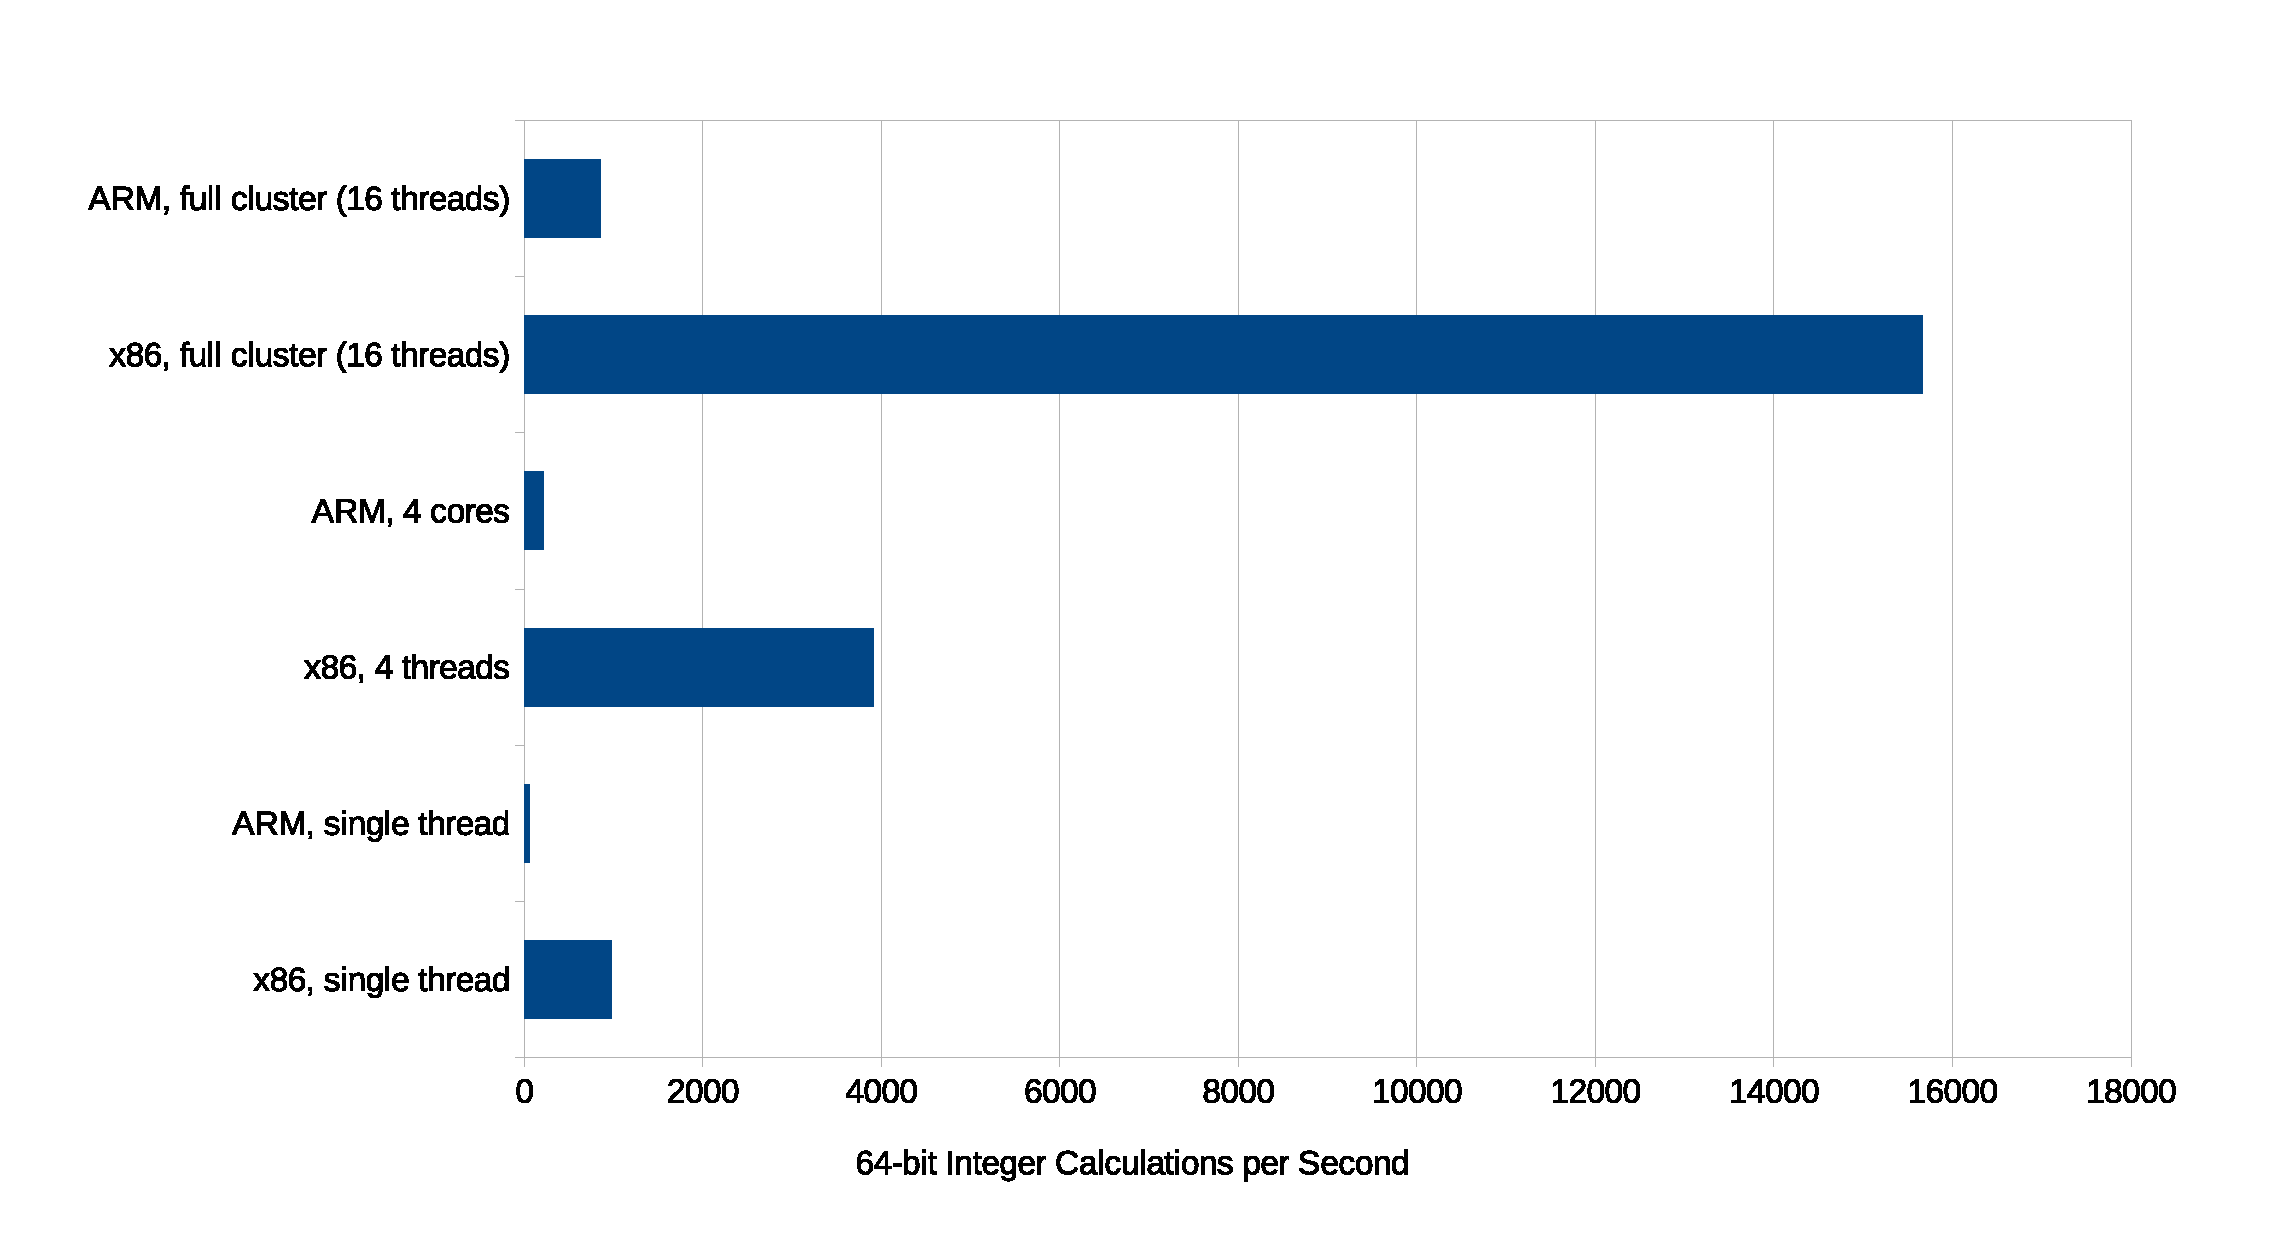
\includegraphics[width=\textwidth]{sysbench_all}
\caption{Sysbench Results}
\label{sysbench-all}
\end{figure}

First, the \verb;sysbench; CPU test was
run on in several threading configurations for 60 seconds per
configuration. This test calculates prime numbers using 64-bit
integers. \textbf{Figure \ref{sysbench-all}} organizes the results of these
tests by the number of threads on which the test was run. Although both
platforms scale well with threads, it is clear that the x86 machine is superior
in 64-bit integer computations. 

\begin{figure}
\centering
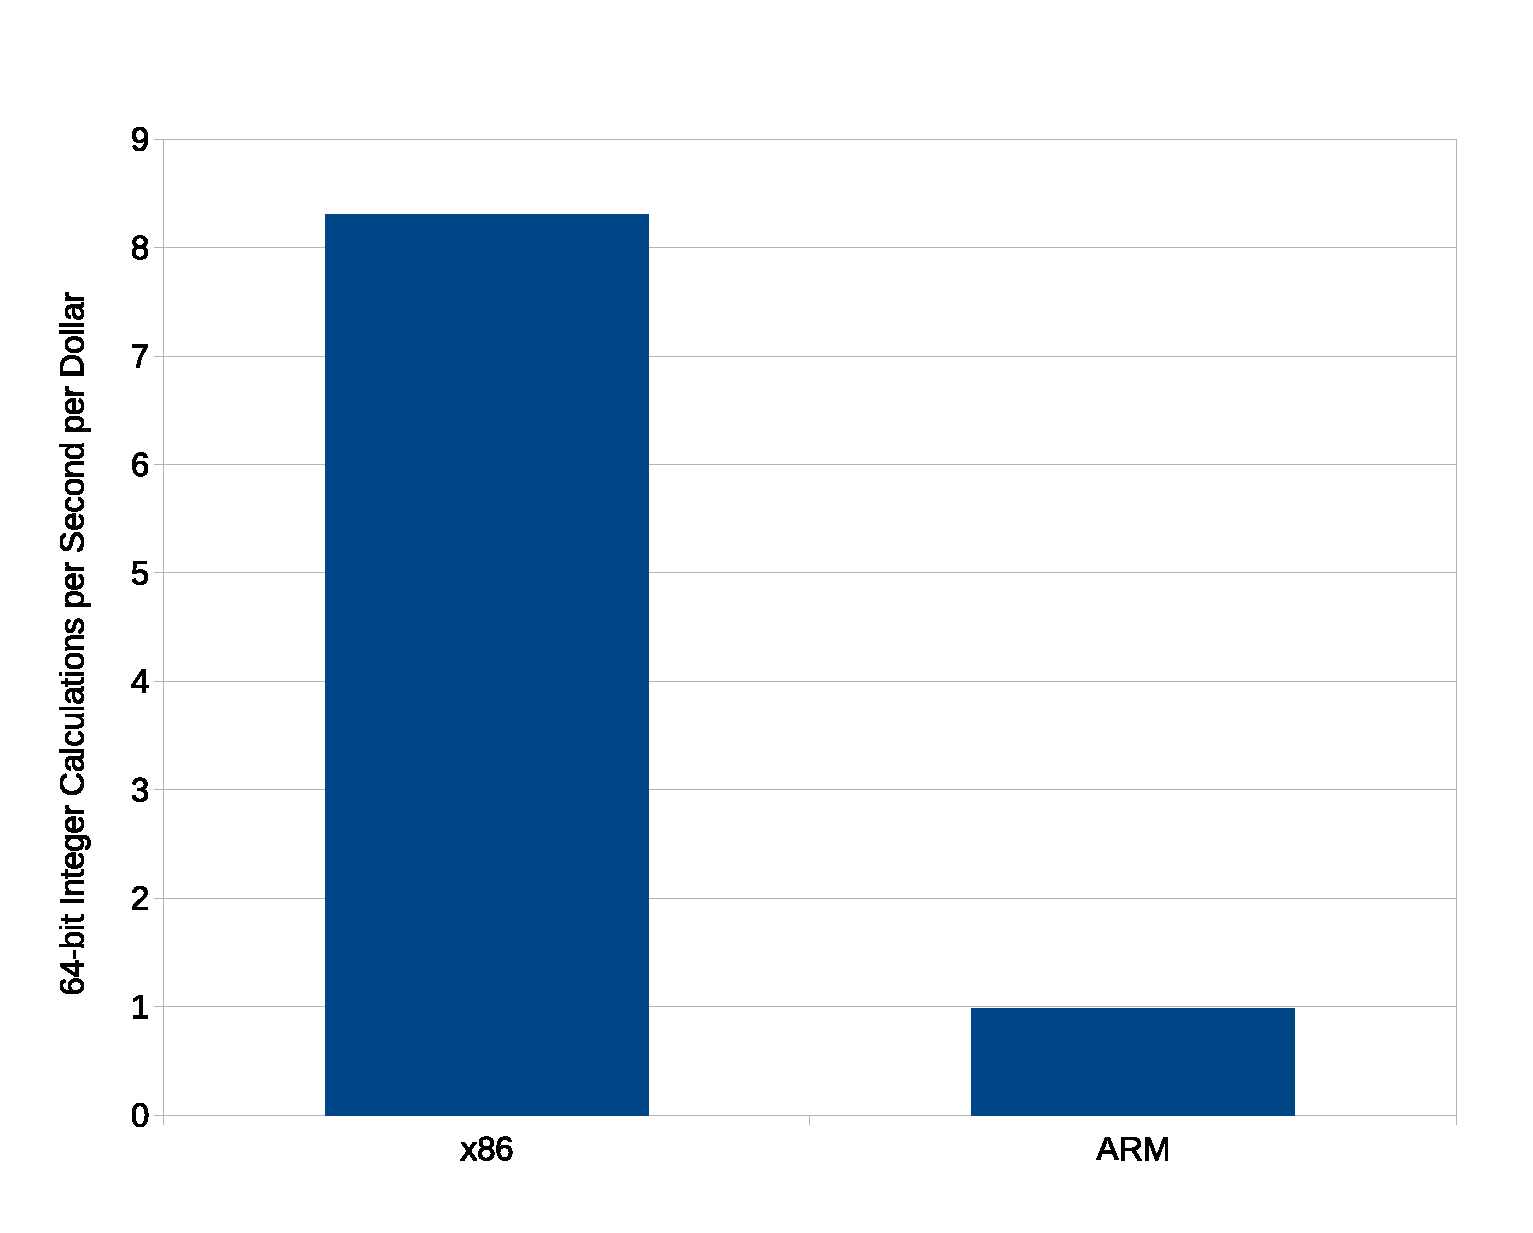
\includegraphics[width=0.75\textwidth]{sysbench_cost}
\caption{Sysbench 64-bit Integer Calculations per Second per Dollar}
\label{sysbench-cost}
\end{figure}

\textbf{Figure \ref{sysbench-cost}} compares the performance per dollar of the
two clusters based on the sysbench results. It is clear that the x86 cluster is
the clear winner in pure compute power for 64-bit integer operations. This is
expected, because the word size of the x86 processor is 64 bits, while the word
size of the ARM processor is 32 bits.

Next, the \verb;nbench; benchmark \cite{nbench} is used to compare performance
in three key areas (integer performance, floating point performance, and memory
performance) in comparison with a baseline machine: an AMD
K6/233. \textbf{Figure \ref{nbench-all}} shows the performance comparison for
both platforms with and without compiler optimizations. The benchmark was
compiled with the GNU C Compiler (\verb;gcc;) on both platforms, with the
\verb;-03; and the \verb;-O0; flags for optimization and no optimization,
respectively.

\begin{figure}
\centering
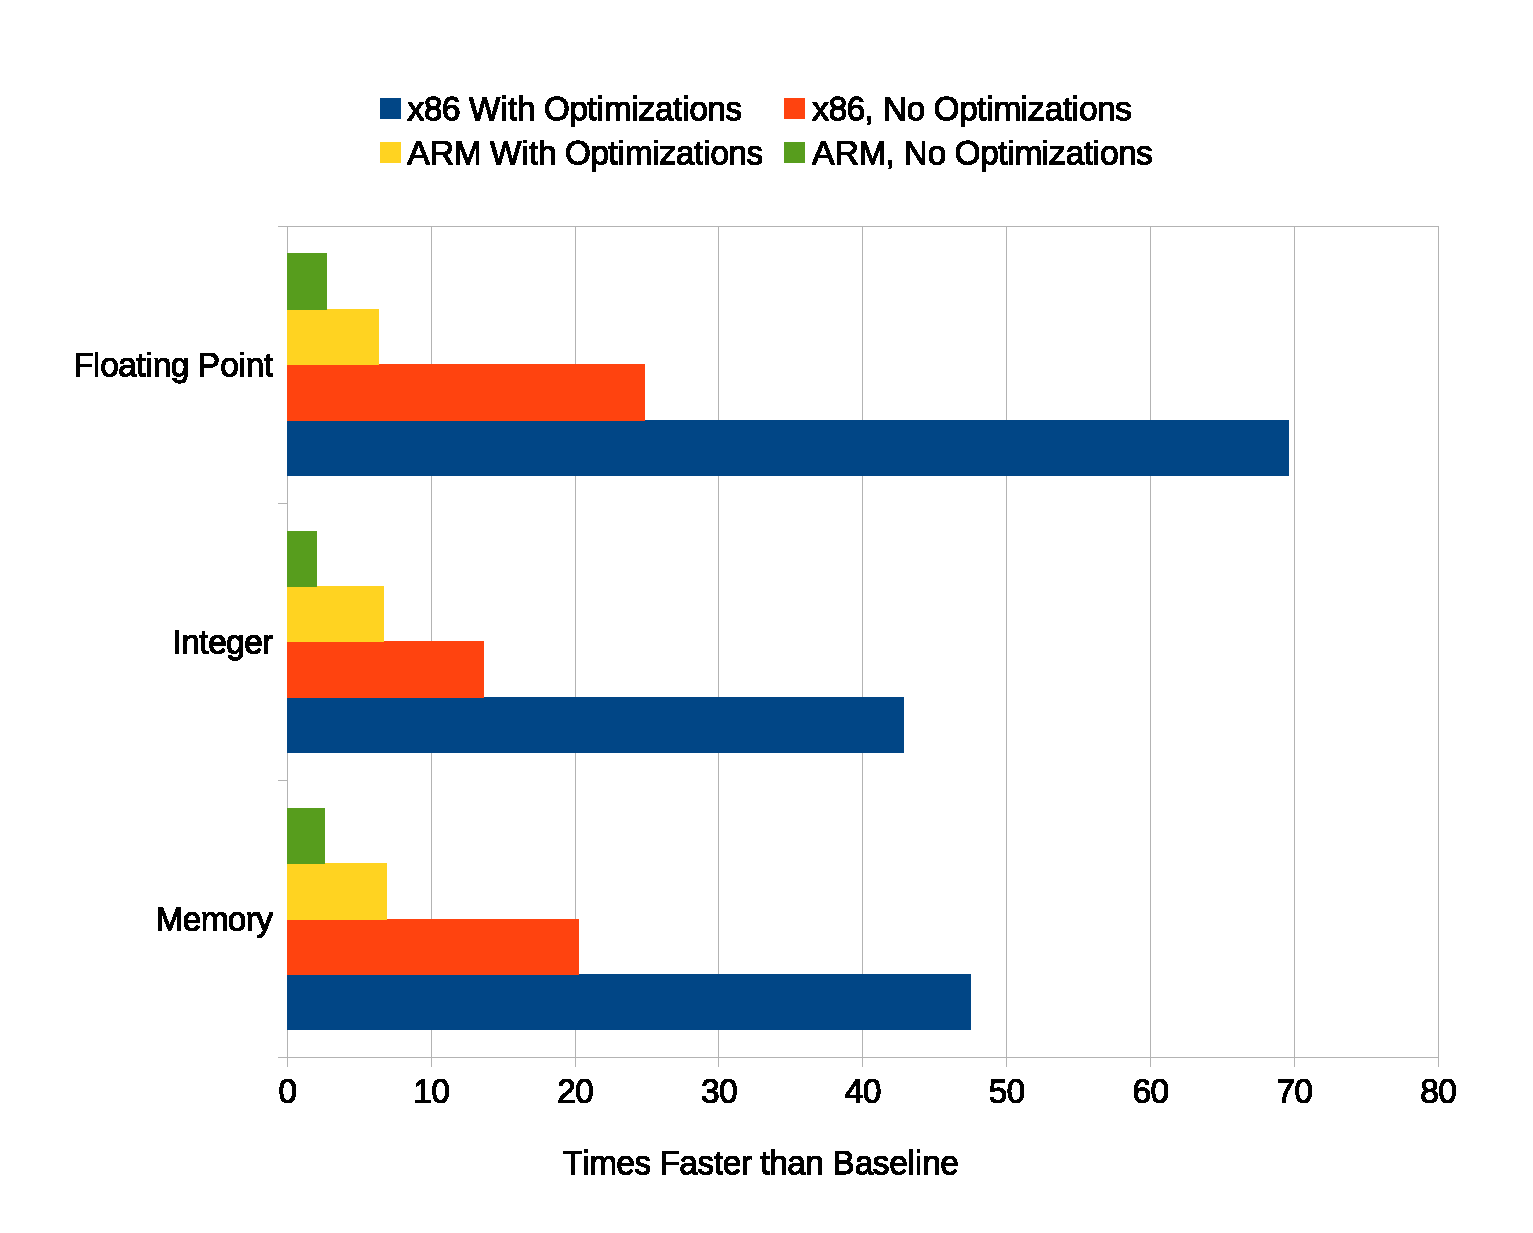
\includegraphics[width=\textwidth]{nbench_all}
\caption{nbench Results}
\label{nbench-all}
\end{figure}

\textbf{Figure \ref{nbench-performance}} sets a new baseline for performance:
our Cortex-A15 machines. The performance results with optimizations are used to
set the performance of the ARM processor at one in each category. \textbf{Figure
  \ref{nbench-cost}} does the same for \verb;nbench; performance per dollar in
each category.

\begin{figure}
\centering
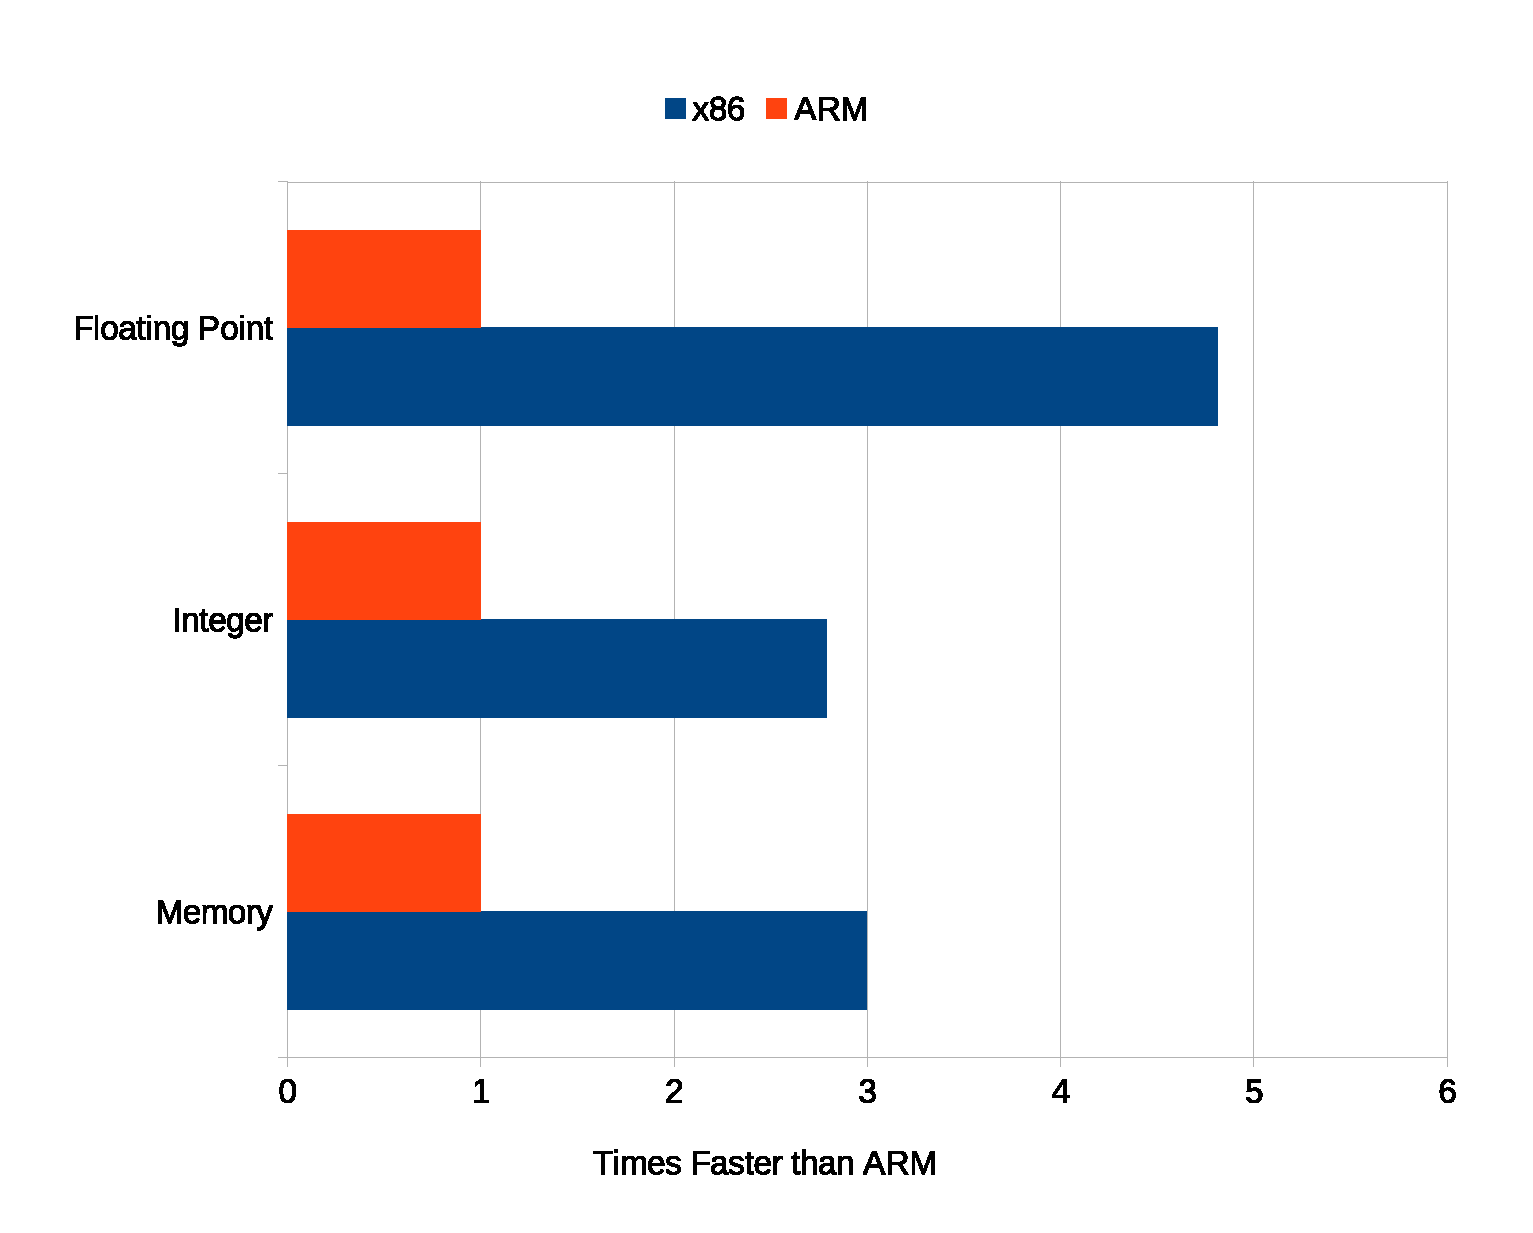
\includegraphics[width=0.75\textwidth]{nbench_performance}
\caption{Normalized nbench Results}
\label{nbench-performance}
\end{figure}


\begin{figure}
\centering
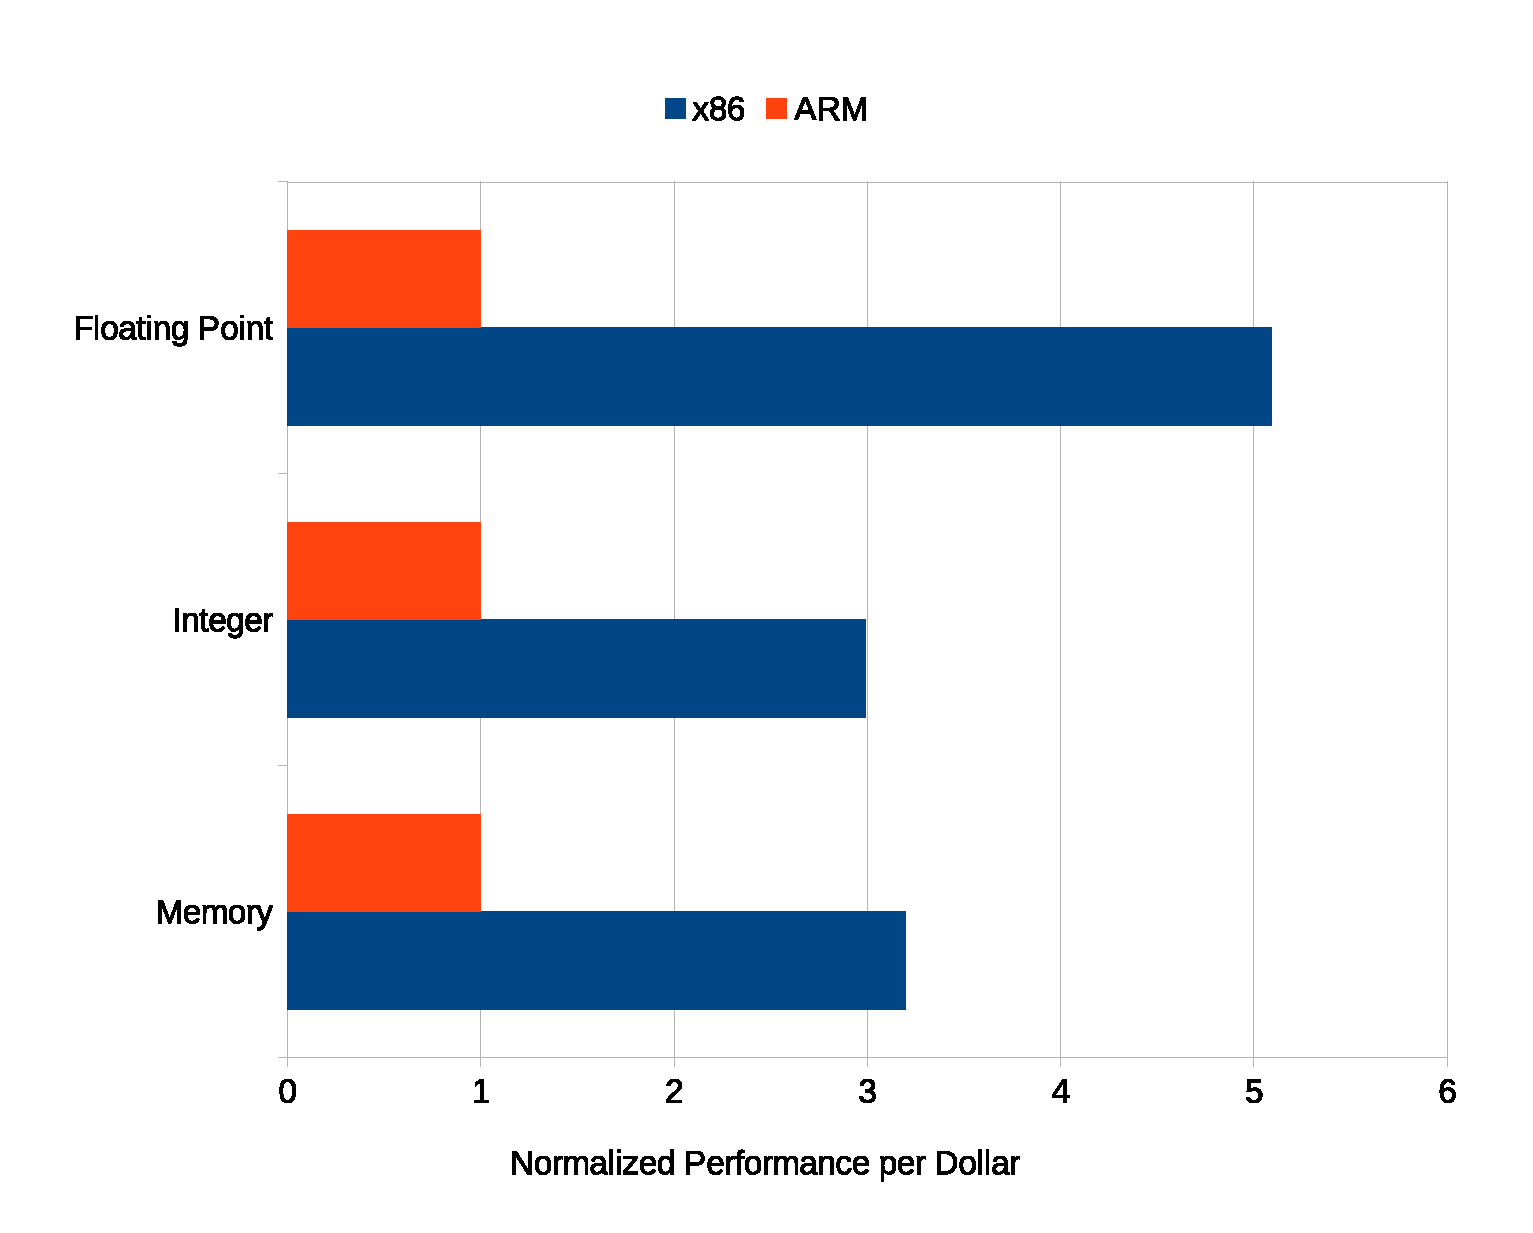
\includegraphics[width=0.75\textwidth]{nbench_cost}
\captionof{figure}{Normalized nbench Performance per Dollar}
\label{nbench-cost}
\end{figure}

In all three performance areas, the x86 CPU more than triples the computation
power per dollar of the ARM CPU as measured by this benchmark. However, one can
expect factors other than raw computing power to determine PDES performance.

\newpage
\chapter{Experimental Results}
\label{results}

We first used micro-benchmarks to demonstrate the performance of the RoCE
transport and polling drivers. We focus on MPI-based benchmarks because these
directly measure the performance available for PDES simulators that use MPI. The
Network Protocol Independent Performance Evaluator (NetPIPE) \cite{NetPIPE}
version 3.7.1 provides an MPI ping-pong benchmark that suits our needs. For more
targeted benchmarking, we turn to the Intel MPI Benchmark (IMB) suite version
3.2.4.

Finally, we used Rensselaer's Optimisitic Simulation System (ROSS) to benchmark
the final cluster's PDES performance.

\section{\textbf{Micro-benchmark Results}}

Preliminary micro-benchmark results from a cluster of two ODROID-U2 nodes are
presented first. Next, the results of similar tests on two of the nodes
comprising the four-node ODROID-XU cluster are shown.

\subsection{\textbf{Two ODROID-U2 Nodes}}

Figures \ref{npmpi-llat} and \ref{npmpi-hlat} show MPI message latency for small
messages and large messages, respectively. Latency over RoCE is 17\% to 31\%
lower than latency over TCP for messages smaller than 260 B. In fact, RoCE
latency remains flat throughout that region, while TCP performance degrades
slowly as message size increases. This trend of identical performance for all
messages from 0 to around 256 B continues throughout this section. We believe
that this is a manifestation of a performance limitation introduced by the
USB-to-Ethernet translation in the LAN9730 hardware.

\begin{figure}[h]
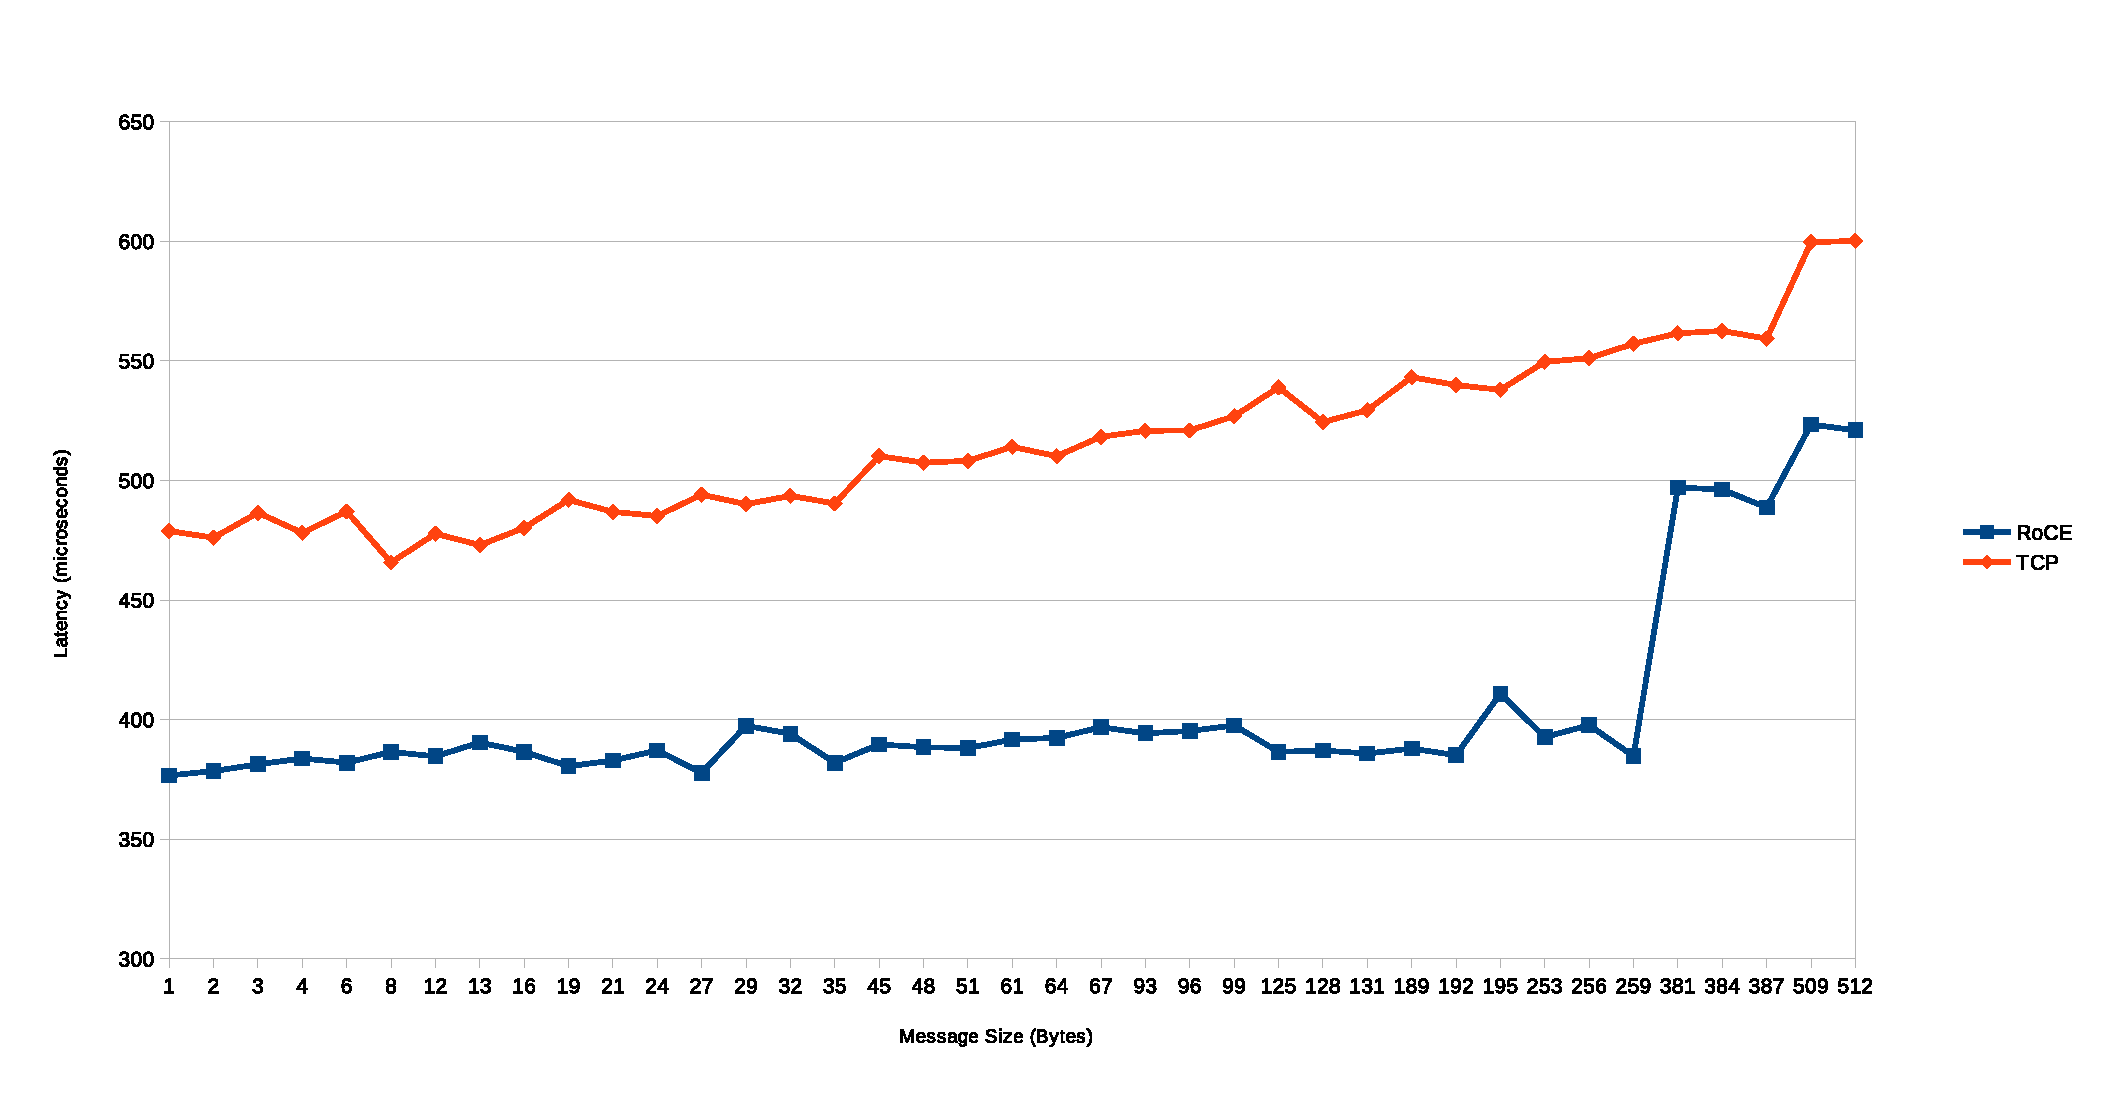
\includegraphics[width=\textwidth]{netpipe_lat_small}
\caption{U2 NetPIPE MPI Latency Results, Small Message Sizes}
\label{npmpi-llat}
\end{figure}

The trend of performance improvement with RoCE continues until message size
rises above 8 KB, after which RoCE latency is significantly higher than TCP
latency.

\begin{figure}[h]
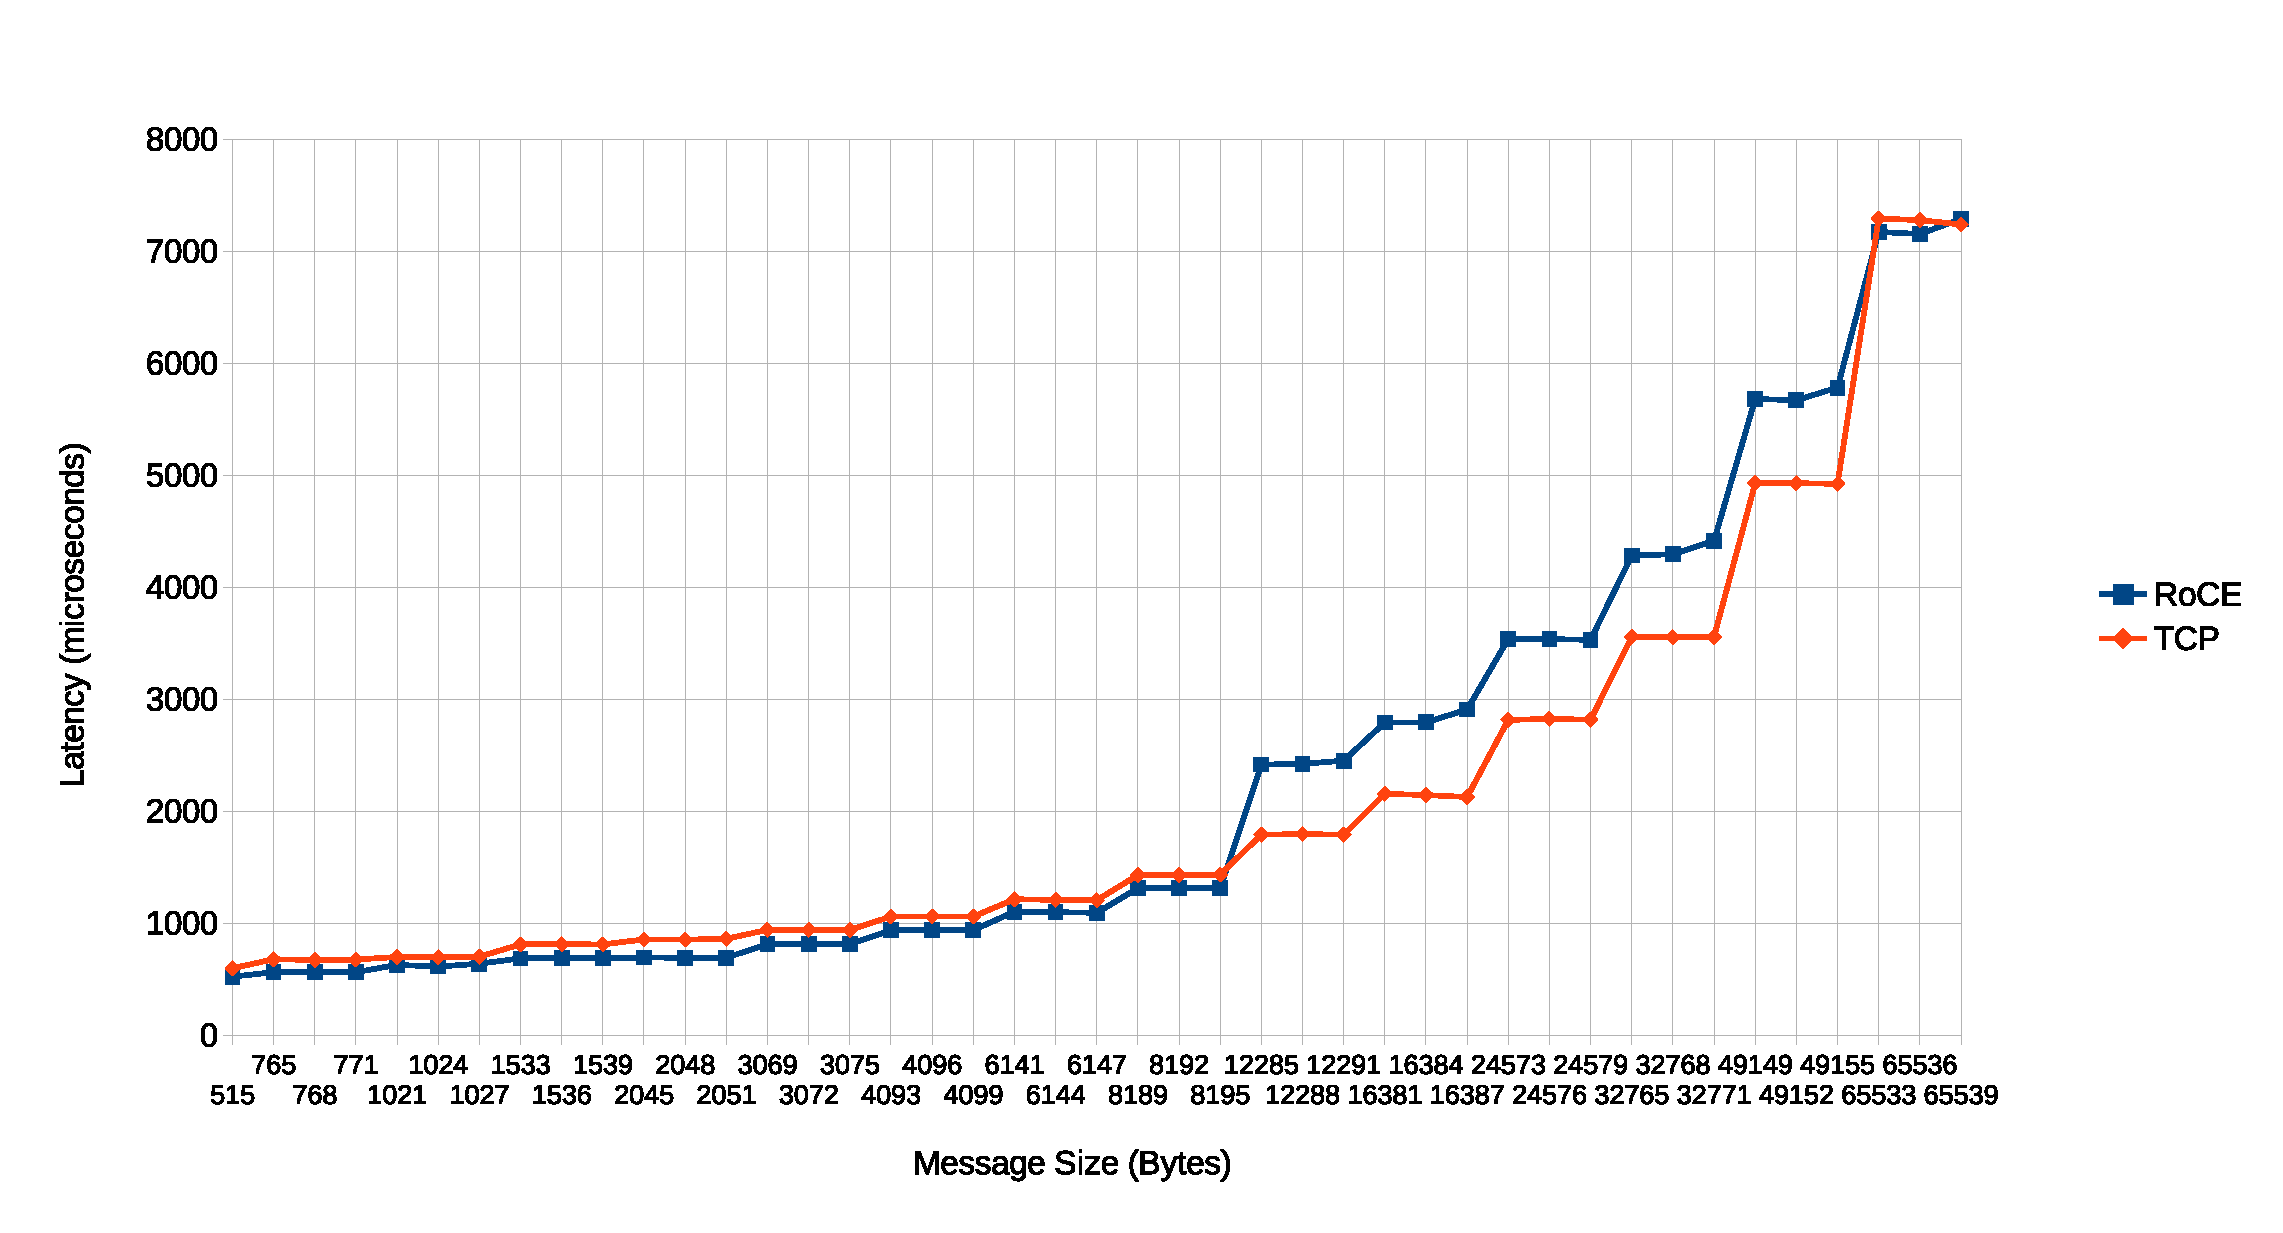
\includegraphics[width=\textwidth]{netpipe_lat_large}
\caption{U2 NetPIPE MPI Latency Results, Large Message Sizes}
\label{npmpi-hlat}
\end{figure}

The MPI bandwidth results in \textbf{Figures \ref{npmpi-lbw}} and
\textbf{\ref{npmpi-hbw}} mirror the latency results. Interestingly, neither TCP
nor RoCE could saturate the 100 Mbps link.

\begin{figure}[h]
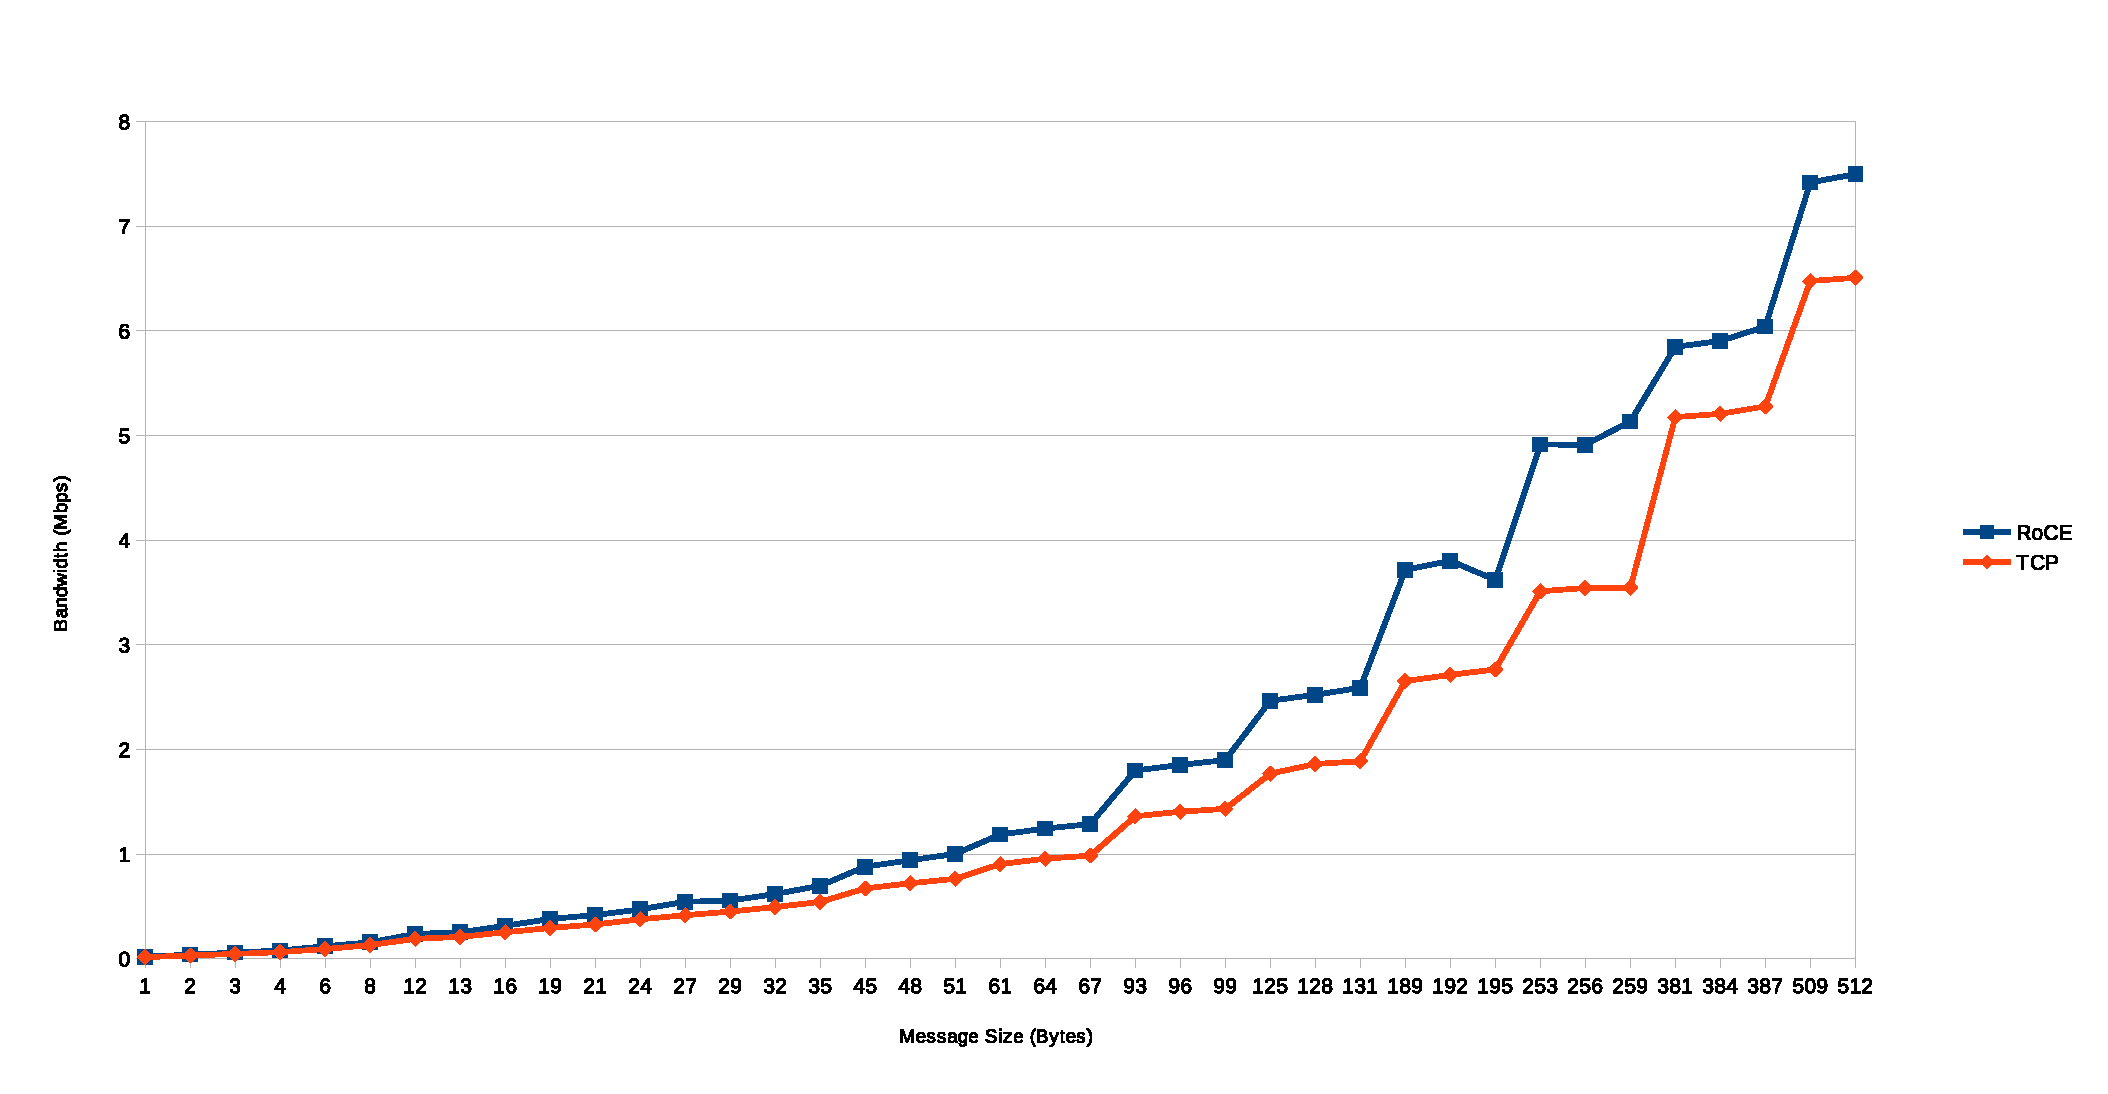
\includegraphics[width=\textwidth]{netpipe_bw_small}
\caption{U2 NetPIPE MPI Bandwidth Results, Small Message Sizes}
\label{npmpi-lbw}
\end{figure}



\begin{figure}[h]
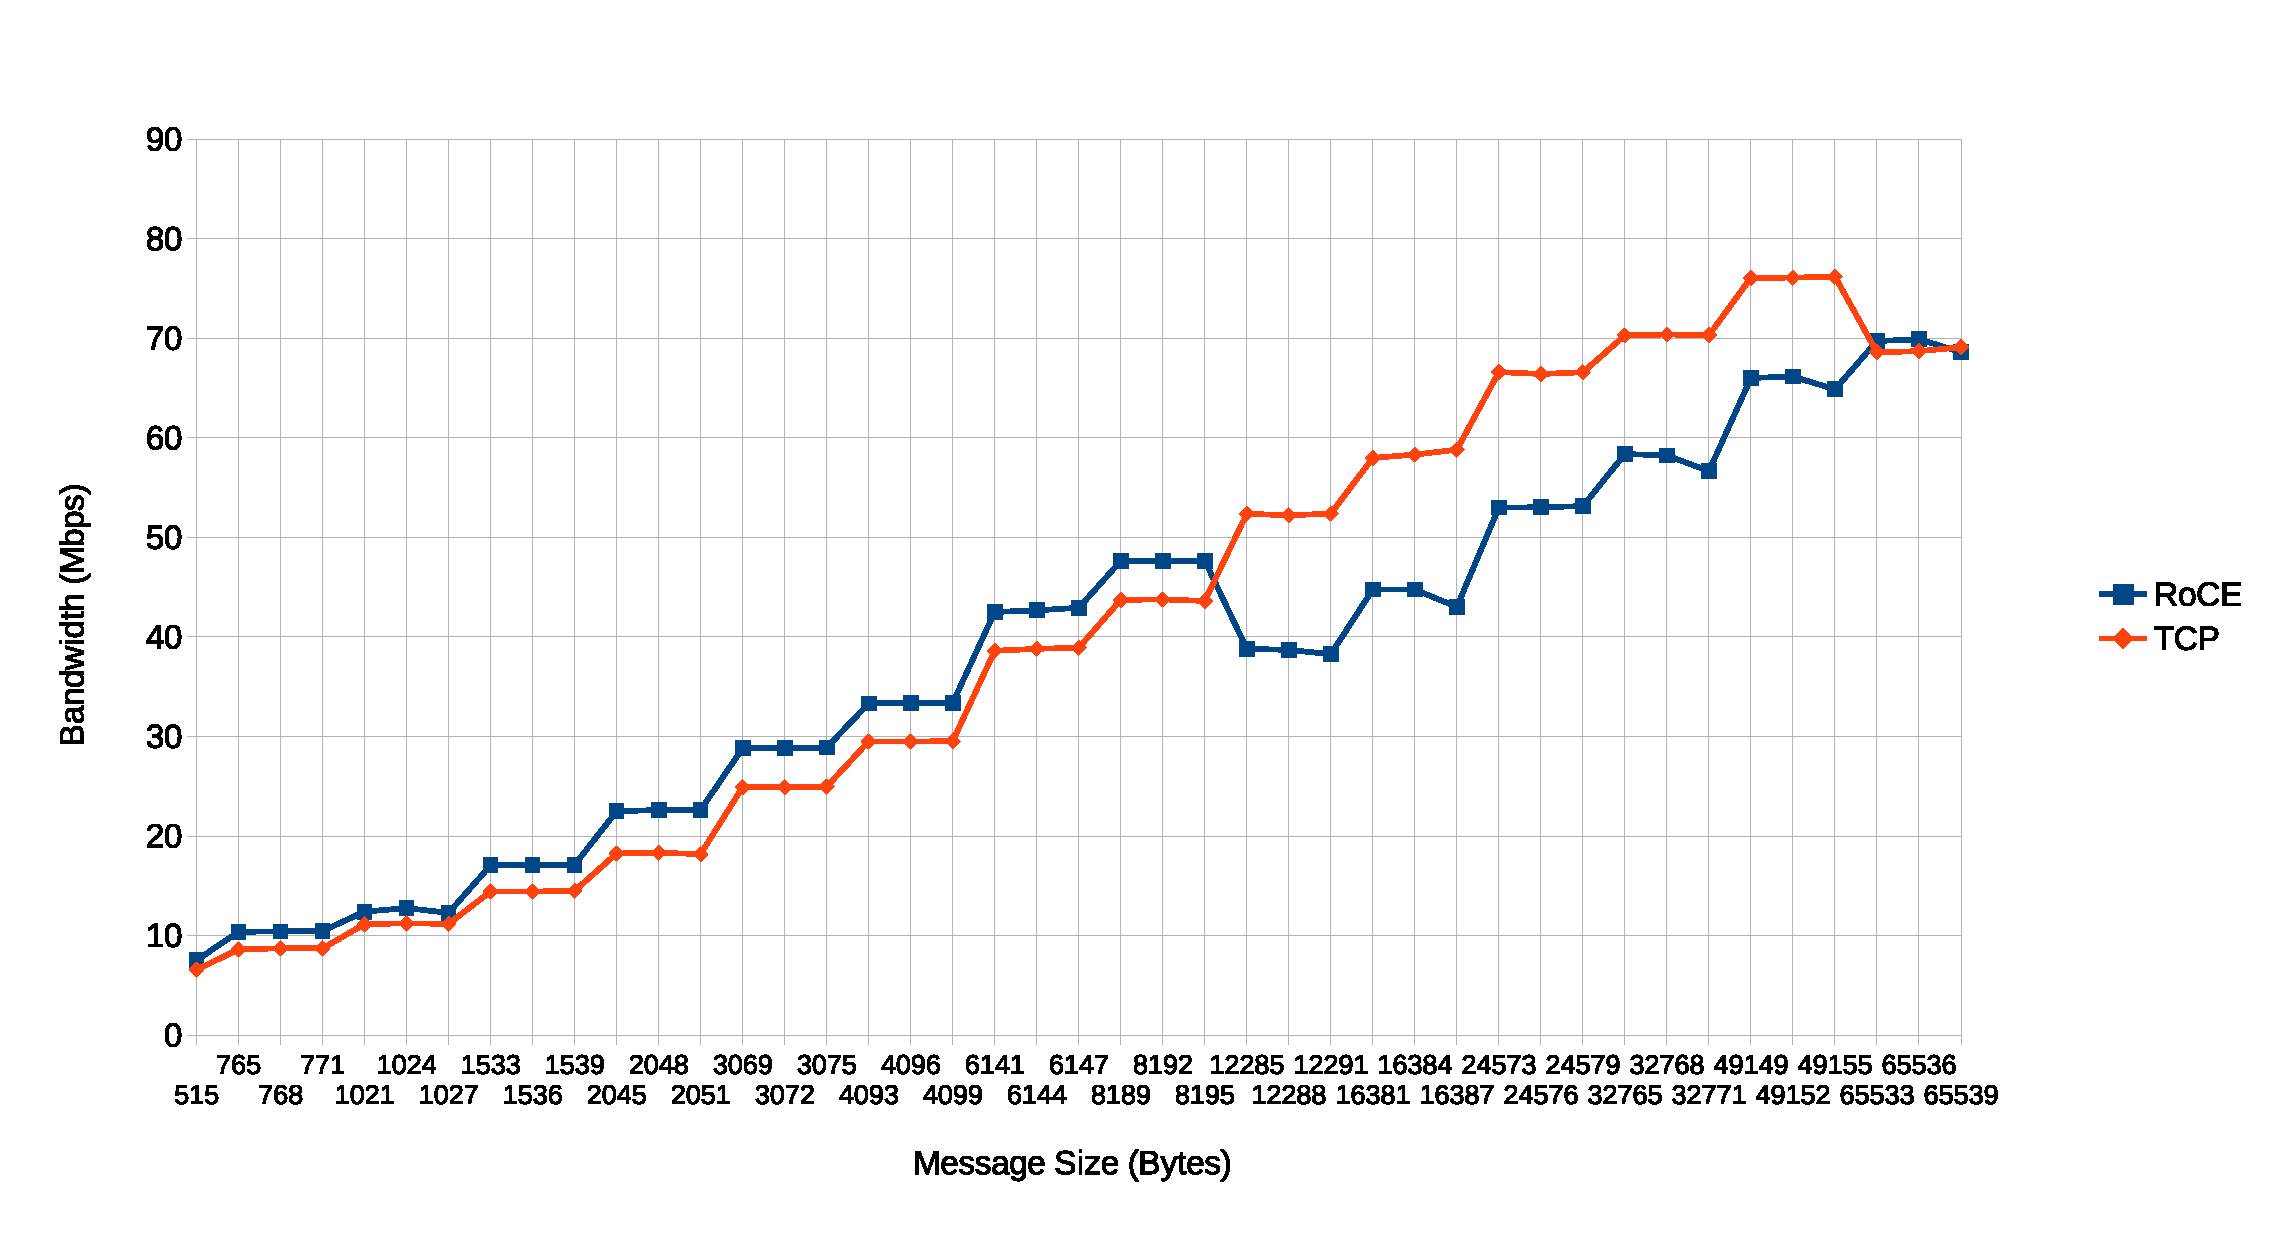
\includegraphics[width=\textwidth]{netpipe_bw_large}
\caption{U2 NetPIPE MPI Bandwidth Results, Large Message Sizes}
\label{npmpi-hbw}
\end{figure}

In order to test transport scalability over MPI in the ODROID platform, we used
the Intel MPI Benchmarks (IMB) suite's ``MultiPingPong'' test with four, six,
and eight MPI processes. This benchmark creates pairs of processes that perform
a standard ping-pong test in parallel with the other pairs. With this tool, we
can test the effects of network communication on inter-process communication by
making some of the process pairs communicate locally on a node and others
communicate over the network. We suspected that the reduced CPU requirements of
the IB transport would lead to slower scaling of latency as network and I/O bus
congestion increases. \textbf{Figure \ref{multipingpong-u2}} supports this
conjecture. In fact, the \verb;rxe; driver appears to thrive in a congested
networking environment, while TCP/IP latency grows steadily. This is surprising
because we expected the average latency of both transports to decrease as low
inter-process communication latencies were averaged with longer network
latencies. Regardless, the context switching associated with TCP appears to have
drastic performance impact on the operation of the Exynos 4412. RoCE appears to
eliminate this problem, with a maximum speedup of over two times TCP.

\begin{figure}[h]
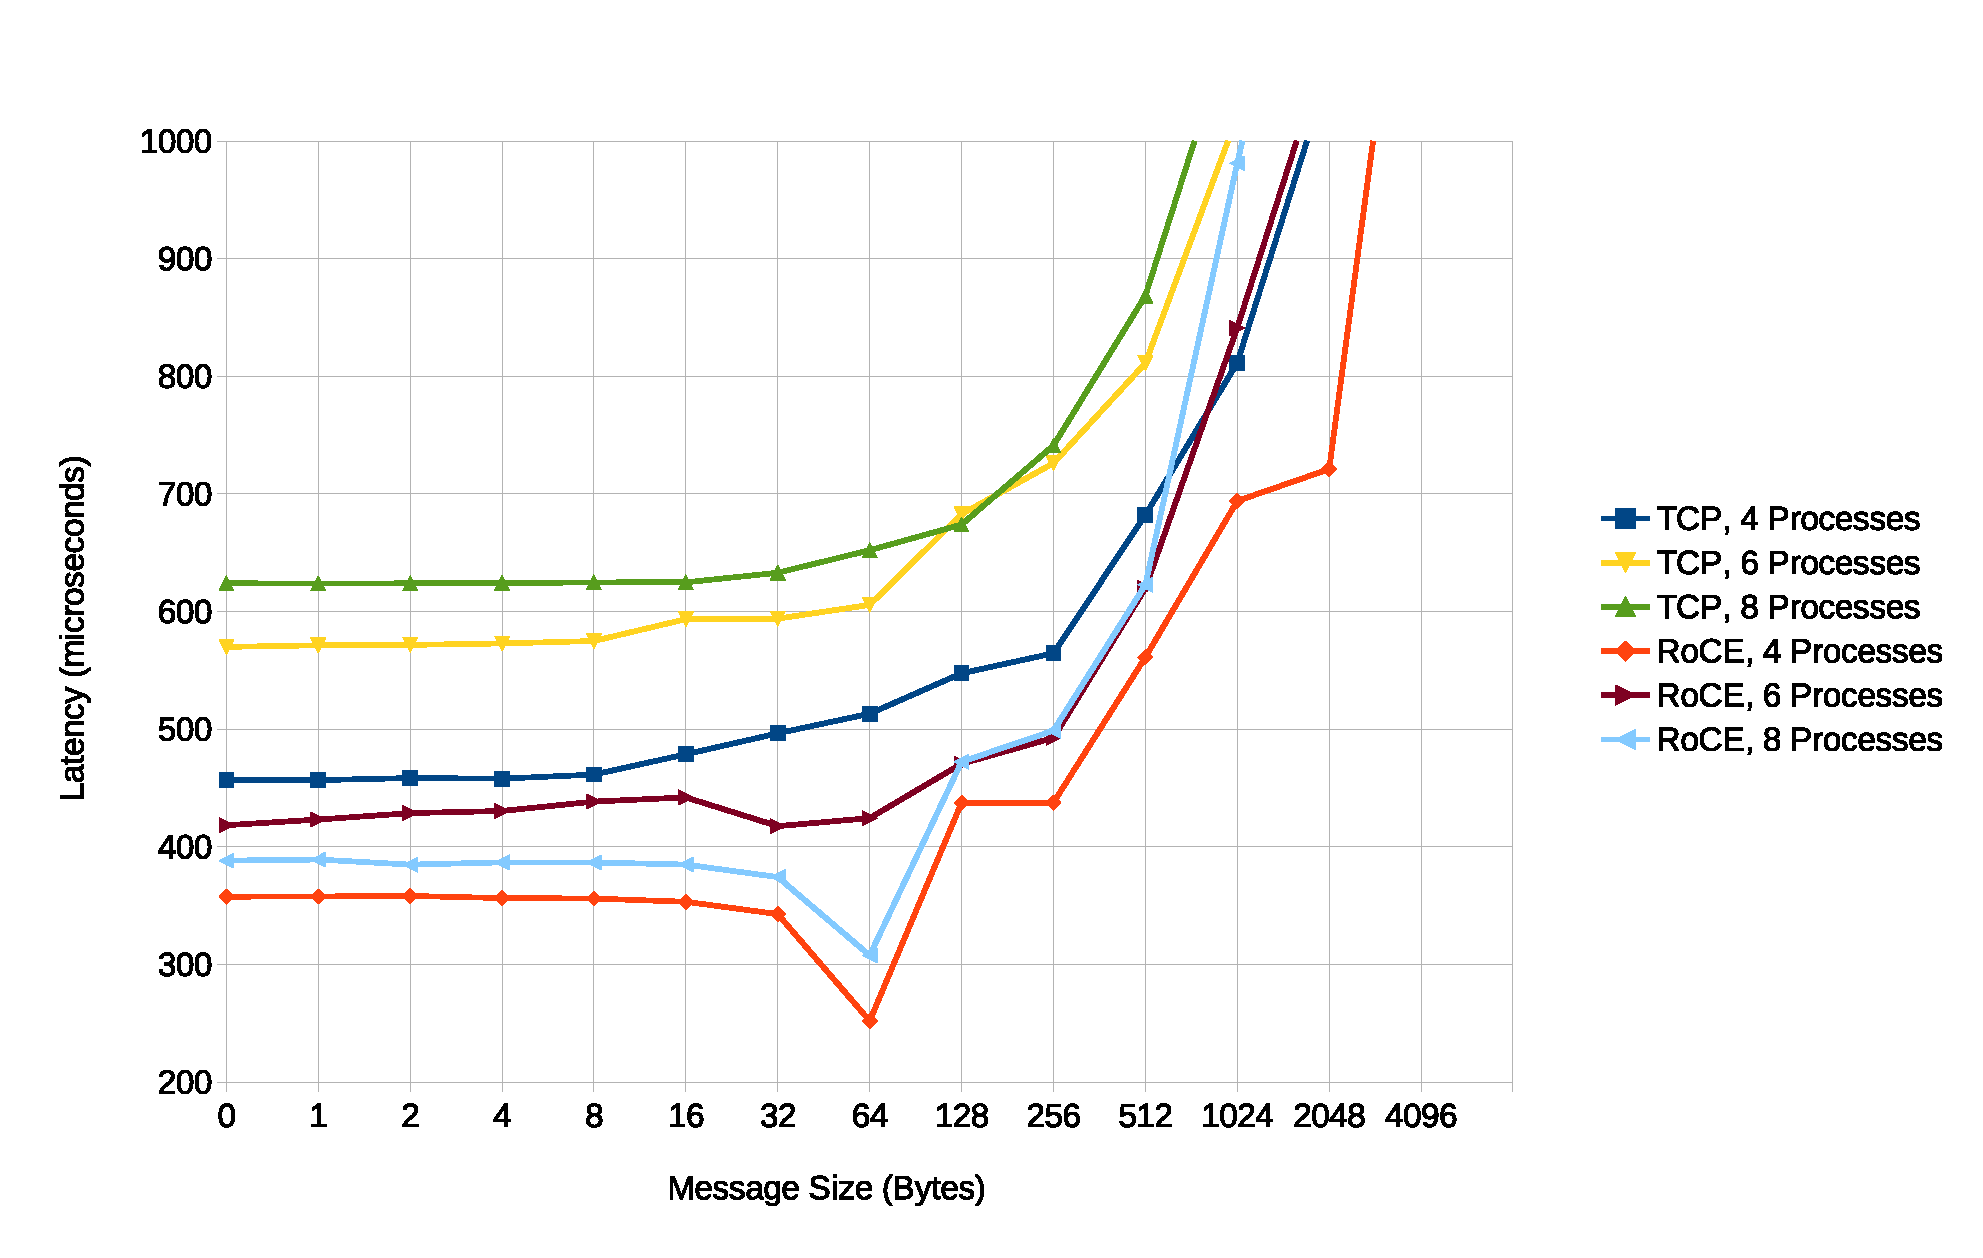
\includegraphics[width=\textwidth]{pingpong_multi_zoom}
\caption{Scaling of U2 Message Latency with Communication Congestion}
\label{multipingpong-u2}
\end{figure}

\subsection{\textbf{Final Cluster}}
\label{final-cluster-benchmarks}

I tested two ODROID-XU nodes equipped with AX88179 Gigabit Ethernet adaptors
using the same NetPIPE and IMB benchmarks that are shown above for the
ODROID-U2. We can see immediately that the purchase of the Gigabit Ethernet
controllers has improved performance drastically, nearly halving our base TCP
small message latency.

\begin{figure}[h]
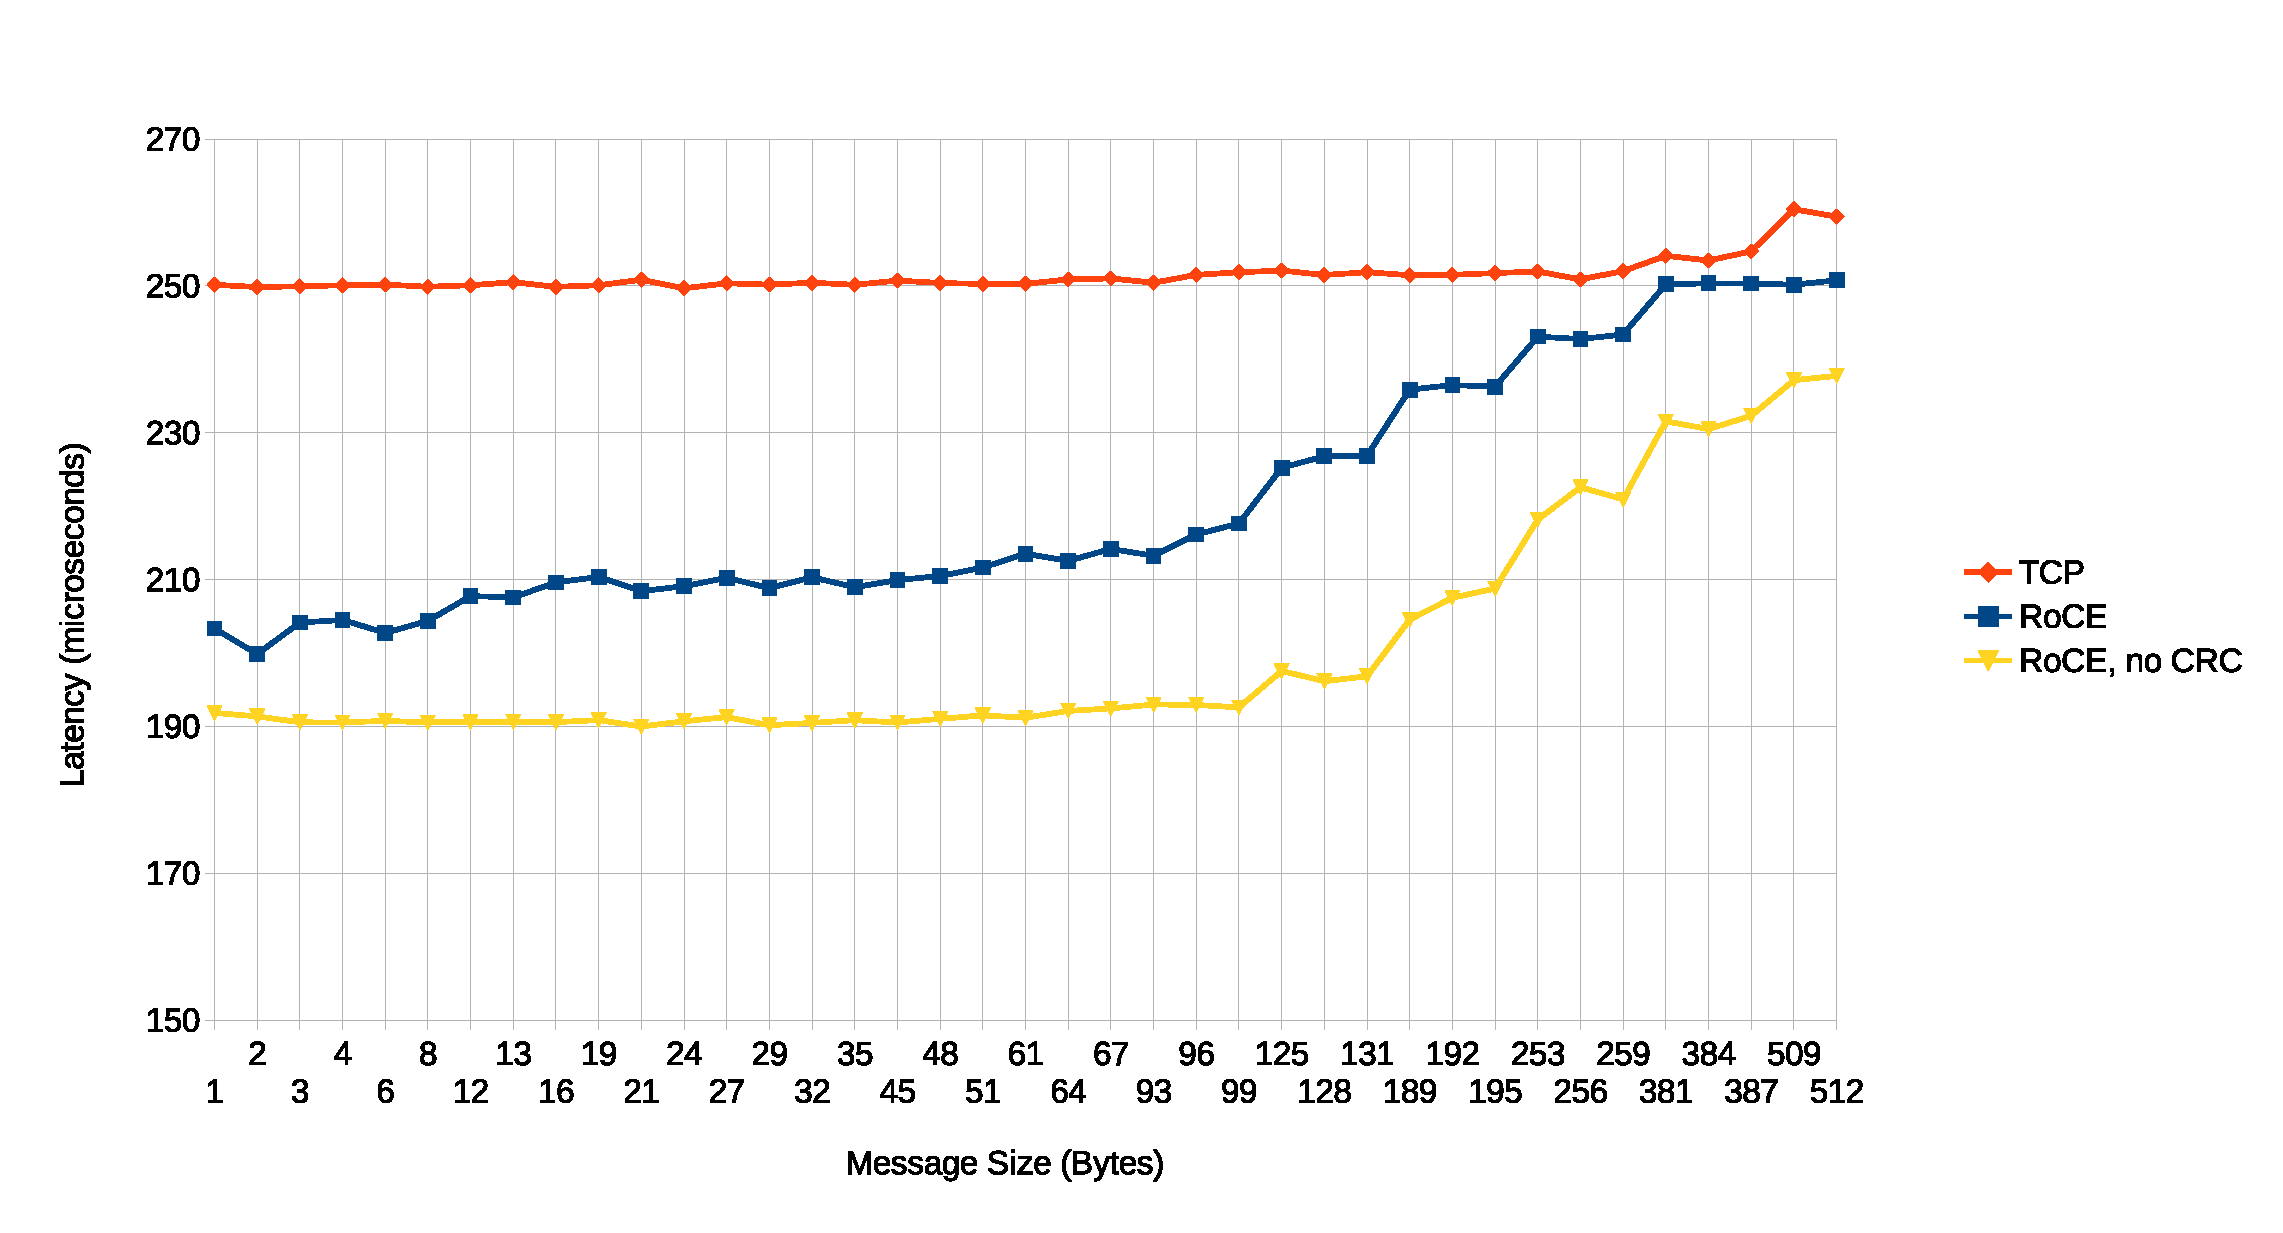
\includegraphics[width=\textwidth]{xu_lat_small}
\caption{XU NetPIPE MPI Latency Results, Small Message Sizes}
\label{xu-lat-small}
\end{figure}

\begin{figure}[h]
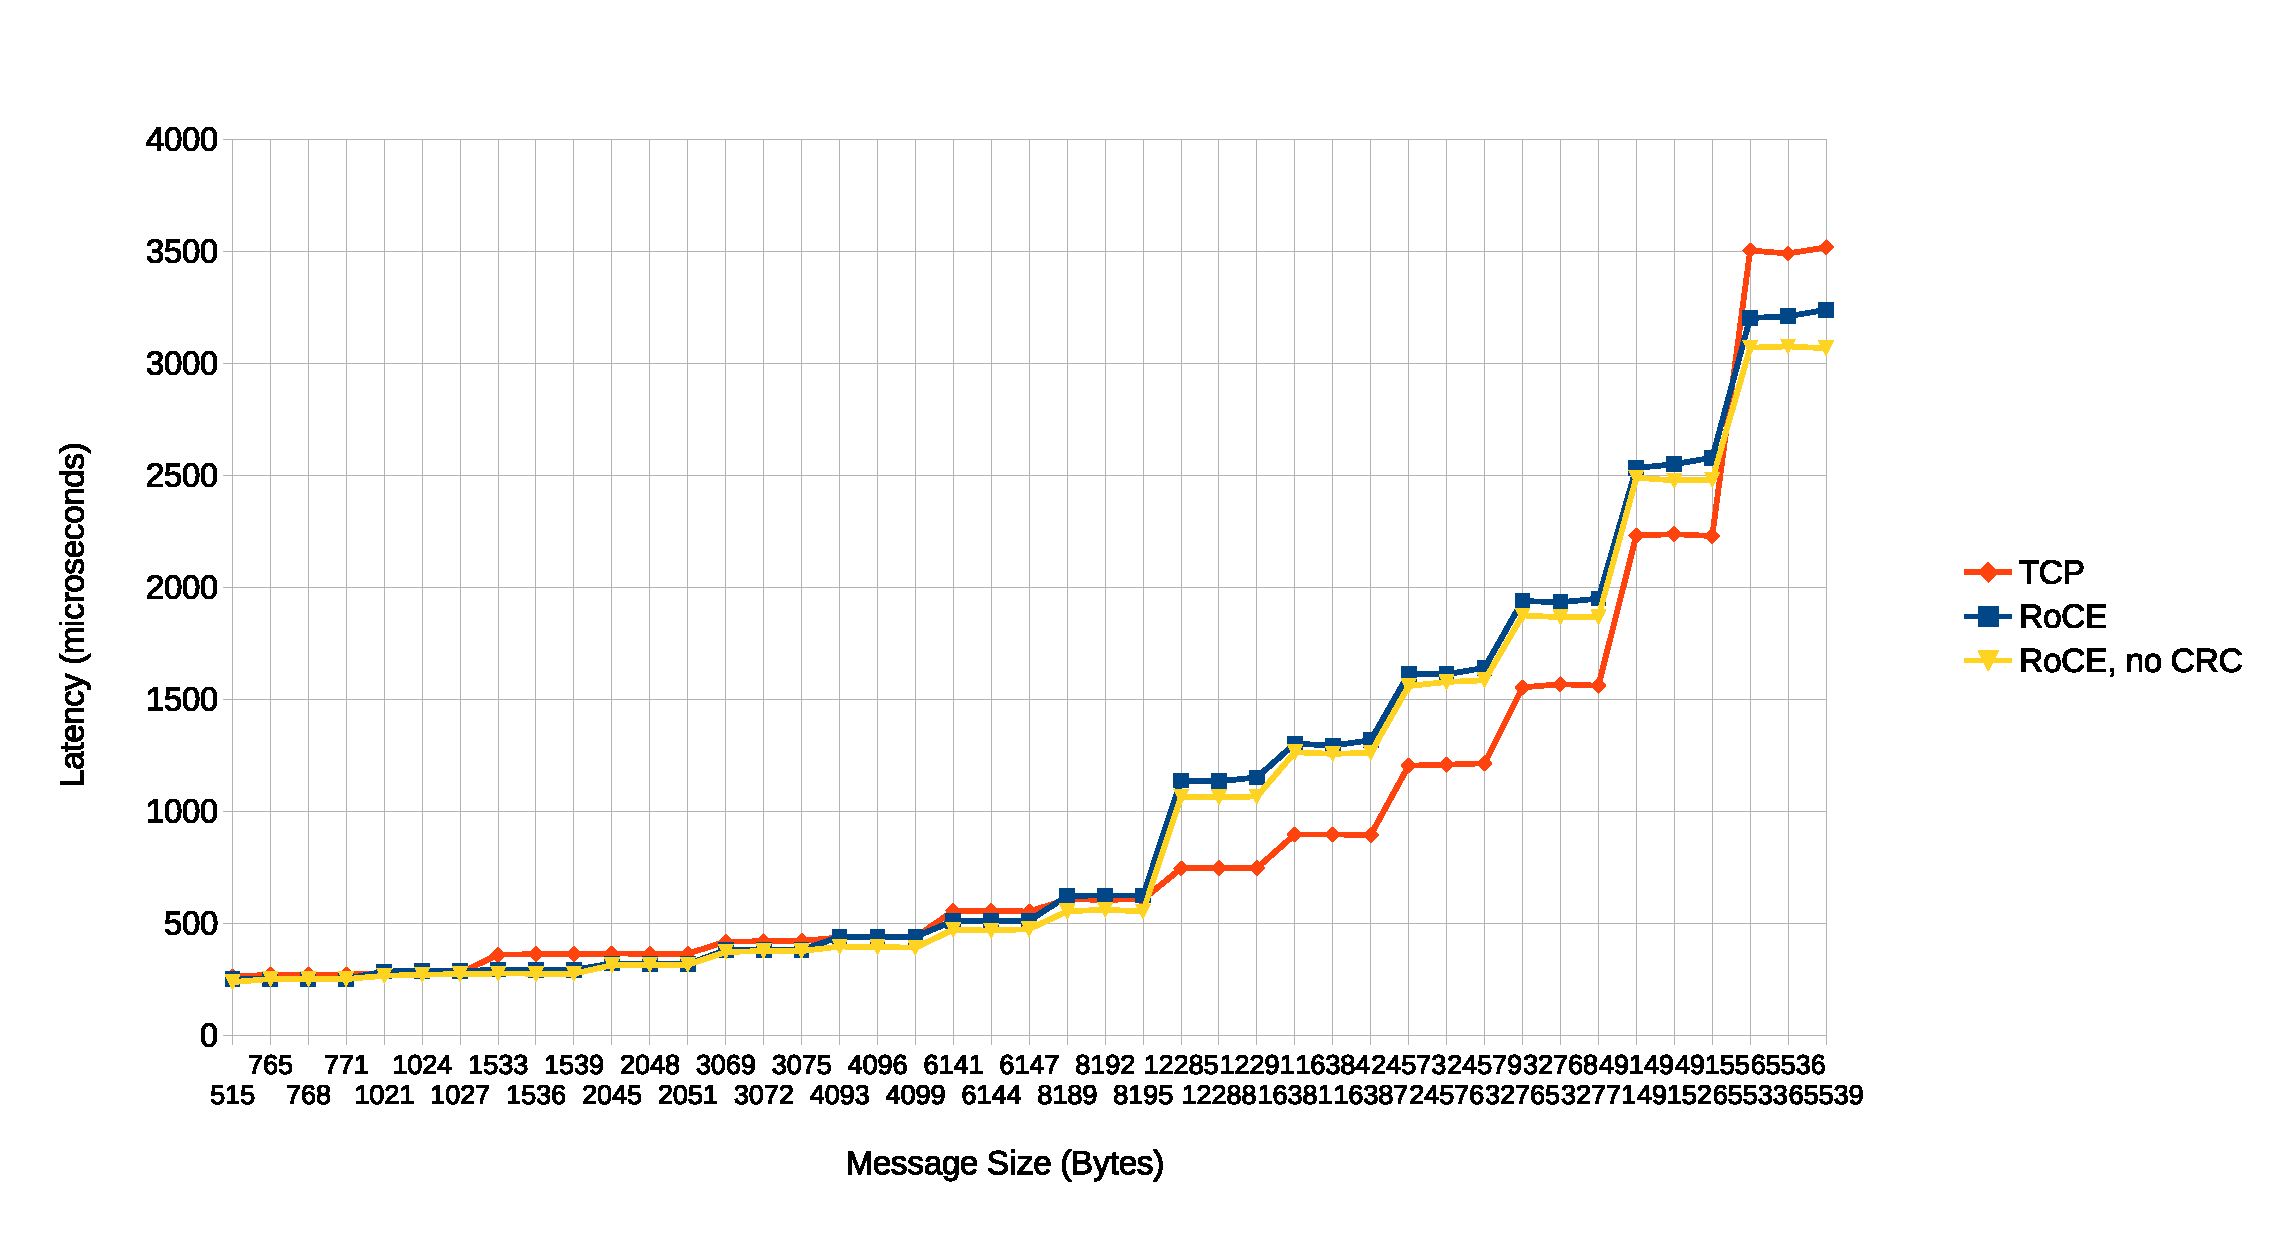
\includegraphics[width=\textwidth]{xu_lat_large}
\caption{XU NetPIPE MPI Latency Results, Large Message Sizes}
\label{xu-lat-large}
\end{figure}

\textbf{Figures \ref{xu-lat-small}} and \textbf{\ref{xu-lat-large}} show the
NetPIPE MPI latency results for two nodes on the ODROID-XU cluster using Gigabit
Ethernet controllers. A minimum message latency of 200 microseconds is an
excellent improvement from the performance observed on the ODROID-U2.

This time, we observe approximately a 25\% decrease in small message latency for
the RoCE transport as compared to TCP. However, the two transports become very
close in performance around message sizes of 384 bytes. This continues until
1024 bytes, where TCP actually overtakes RoCE briefly. Strangely, this entire
trend repeats for the range from 1024 to 4096 bytes and again from 4096 bytes to
8192 bytes. After 8 KB, RoCE latency is significantly higher than TCP latency
until 64 KB, where RoCE again takes the lead.

I speculated that these results could be caused by the calculation of the Cyclic
Redundance Check (CRC) for each RoCE packet. This would explain the performance
sensitifity to certain message sizes. In order to test this hypothesis, I ran
the same tests again with the RoCE CRC disabled. Sure enough, performance
improved compared to RoCE with CRC enabled, returning to data trends similar to
what we observed from the ODROID-U2. Note that disabling the CRC does not reduce
packet size; it merely bypasses the actual computation of the CRC. Although CRC
computation is considered inexpensive, it clearly has a measurable effect on
both latency and bandwidth performance here.

Returning to the ODROID-U2 and disabling the RoCE CRC yielded no significant
performance changes. This implies that the reduction in latency from the Gigabit
Ethernet controller exposed some of the performance costs of the \verb;rxe; CRC
algorithm that were previously hidden by the high latency of the LAN9730
ethernet controller. In accordance with this finding, our PDES tests will be run
with RoCE CRC disabled.

\begin{figure}[h]
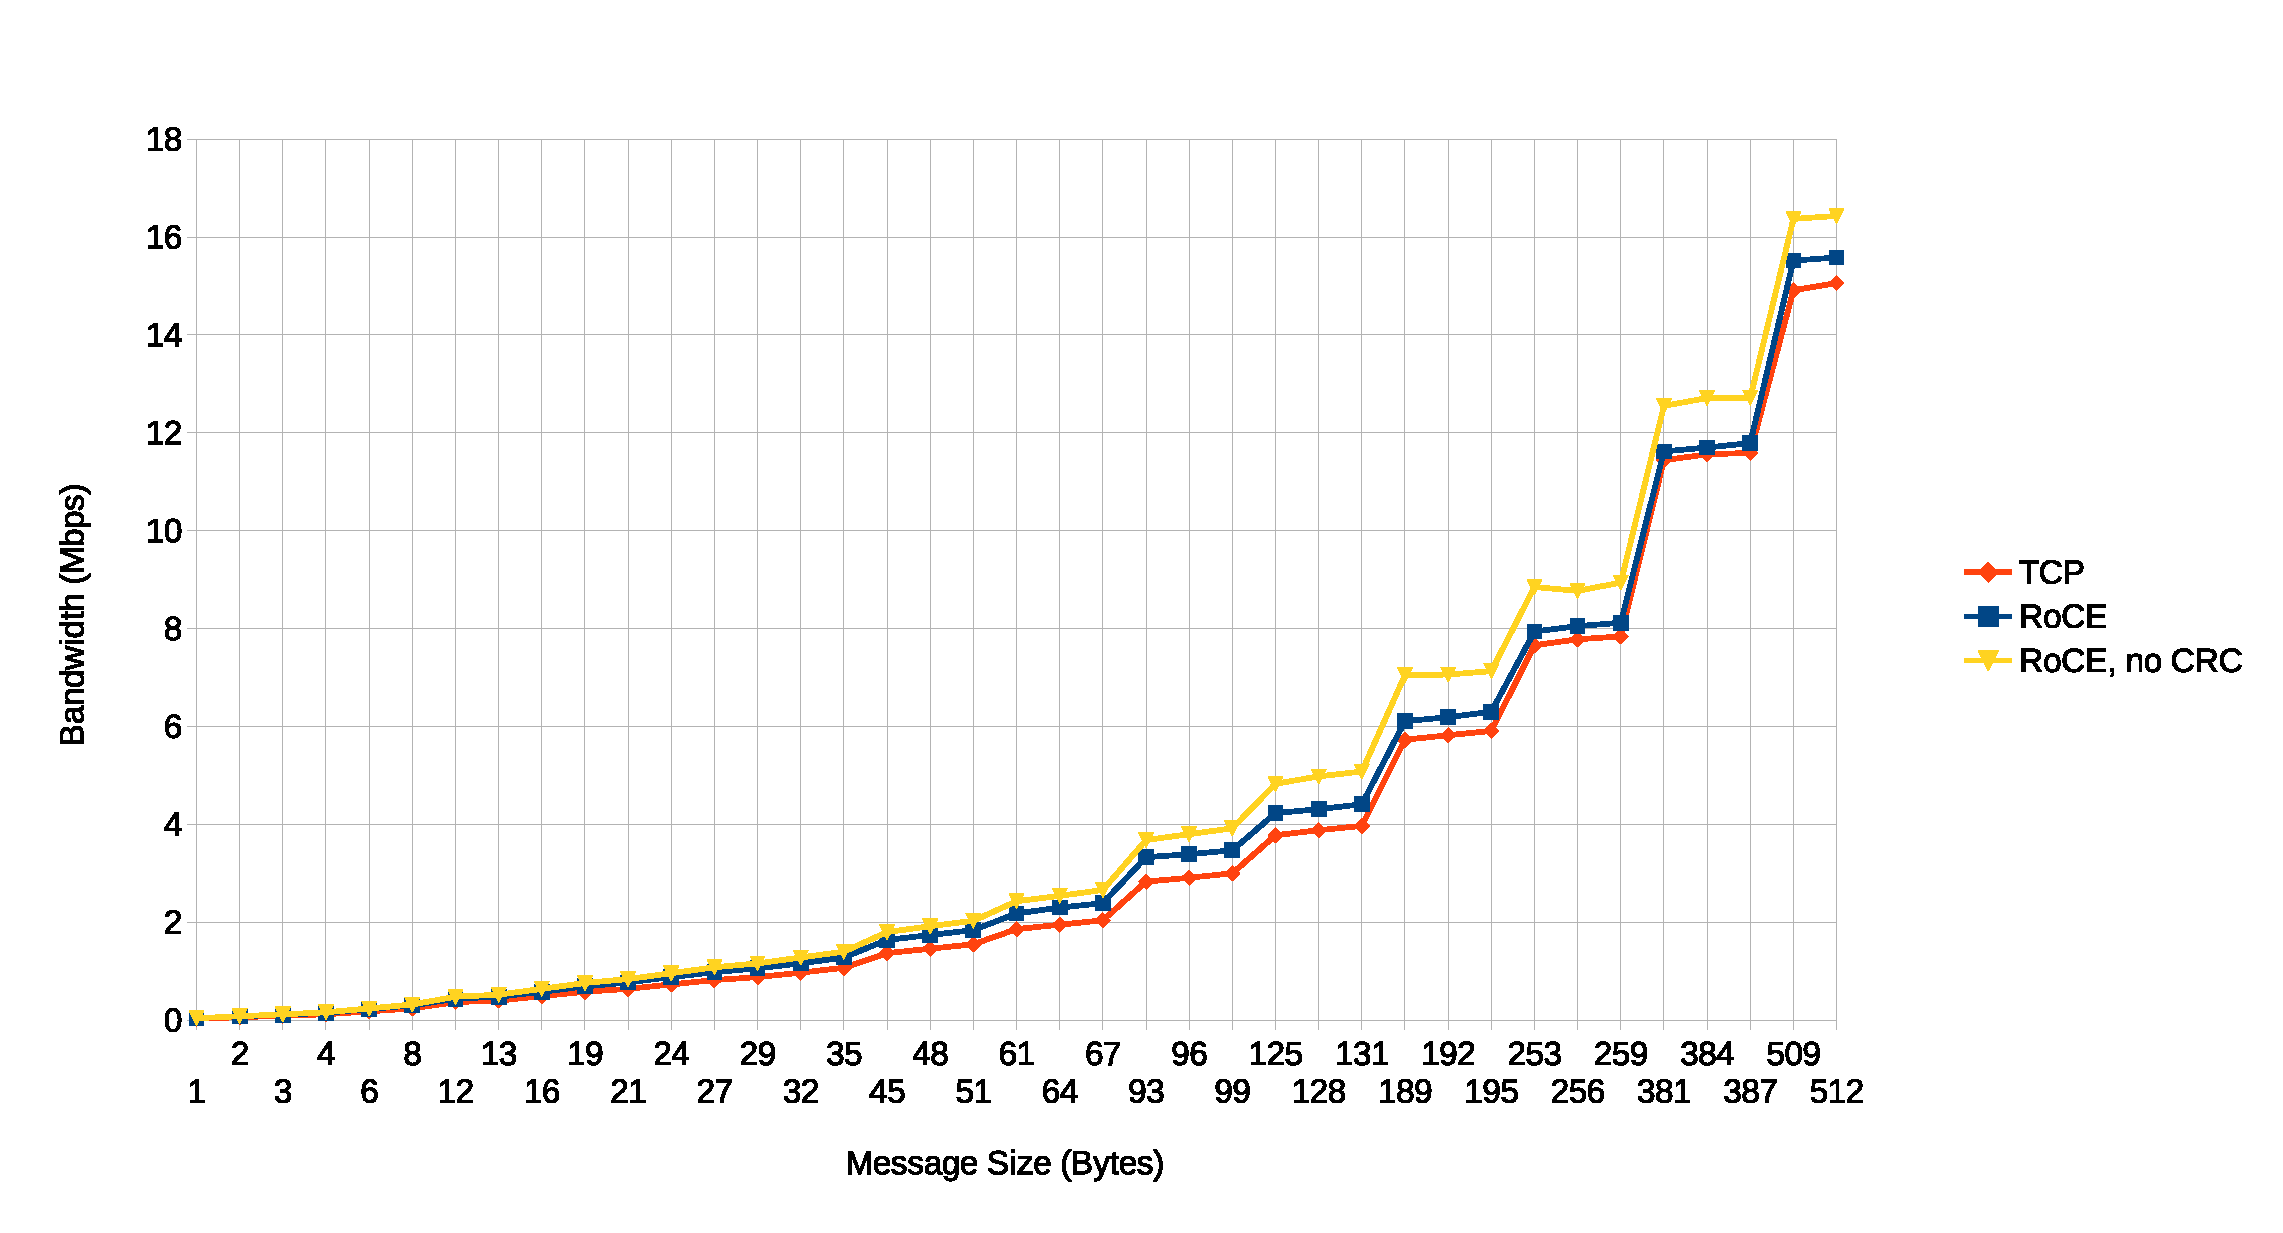
\includegraphics[width=\textwidth]{xu_bw_small}
\caption{XU NetPIPE MPI Bandwidth Results, Small Message Sizes}
\label{xu-bw-small}
\end{figure}

\begin{figure}[h]
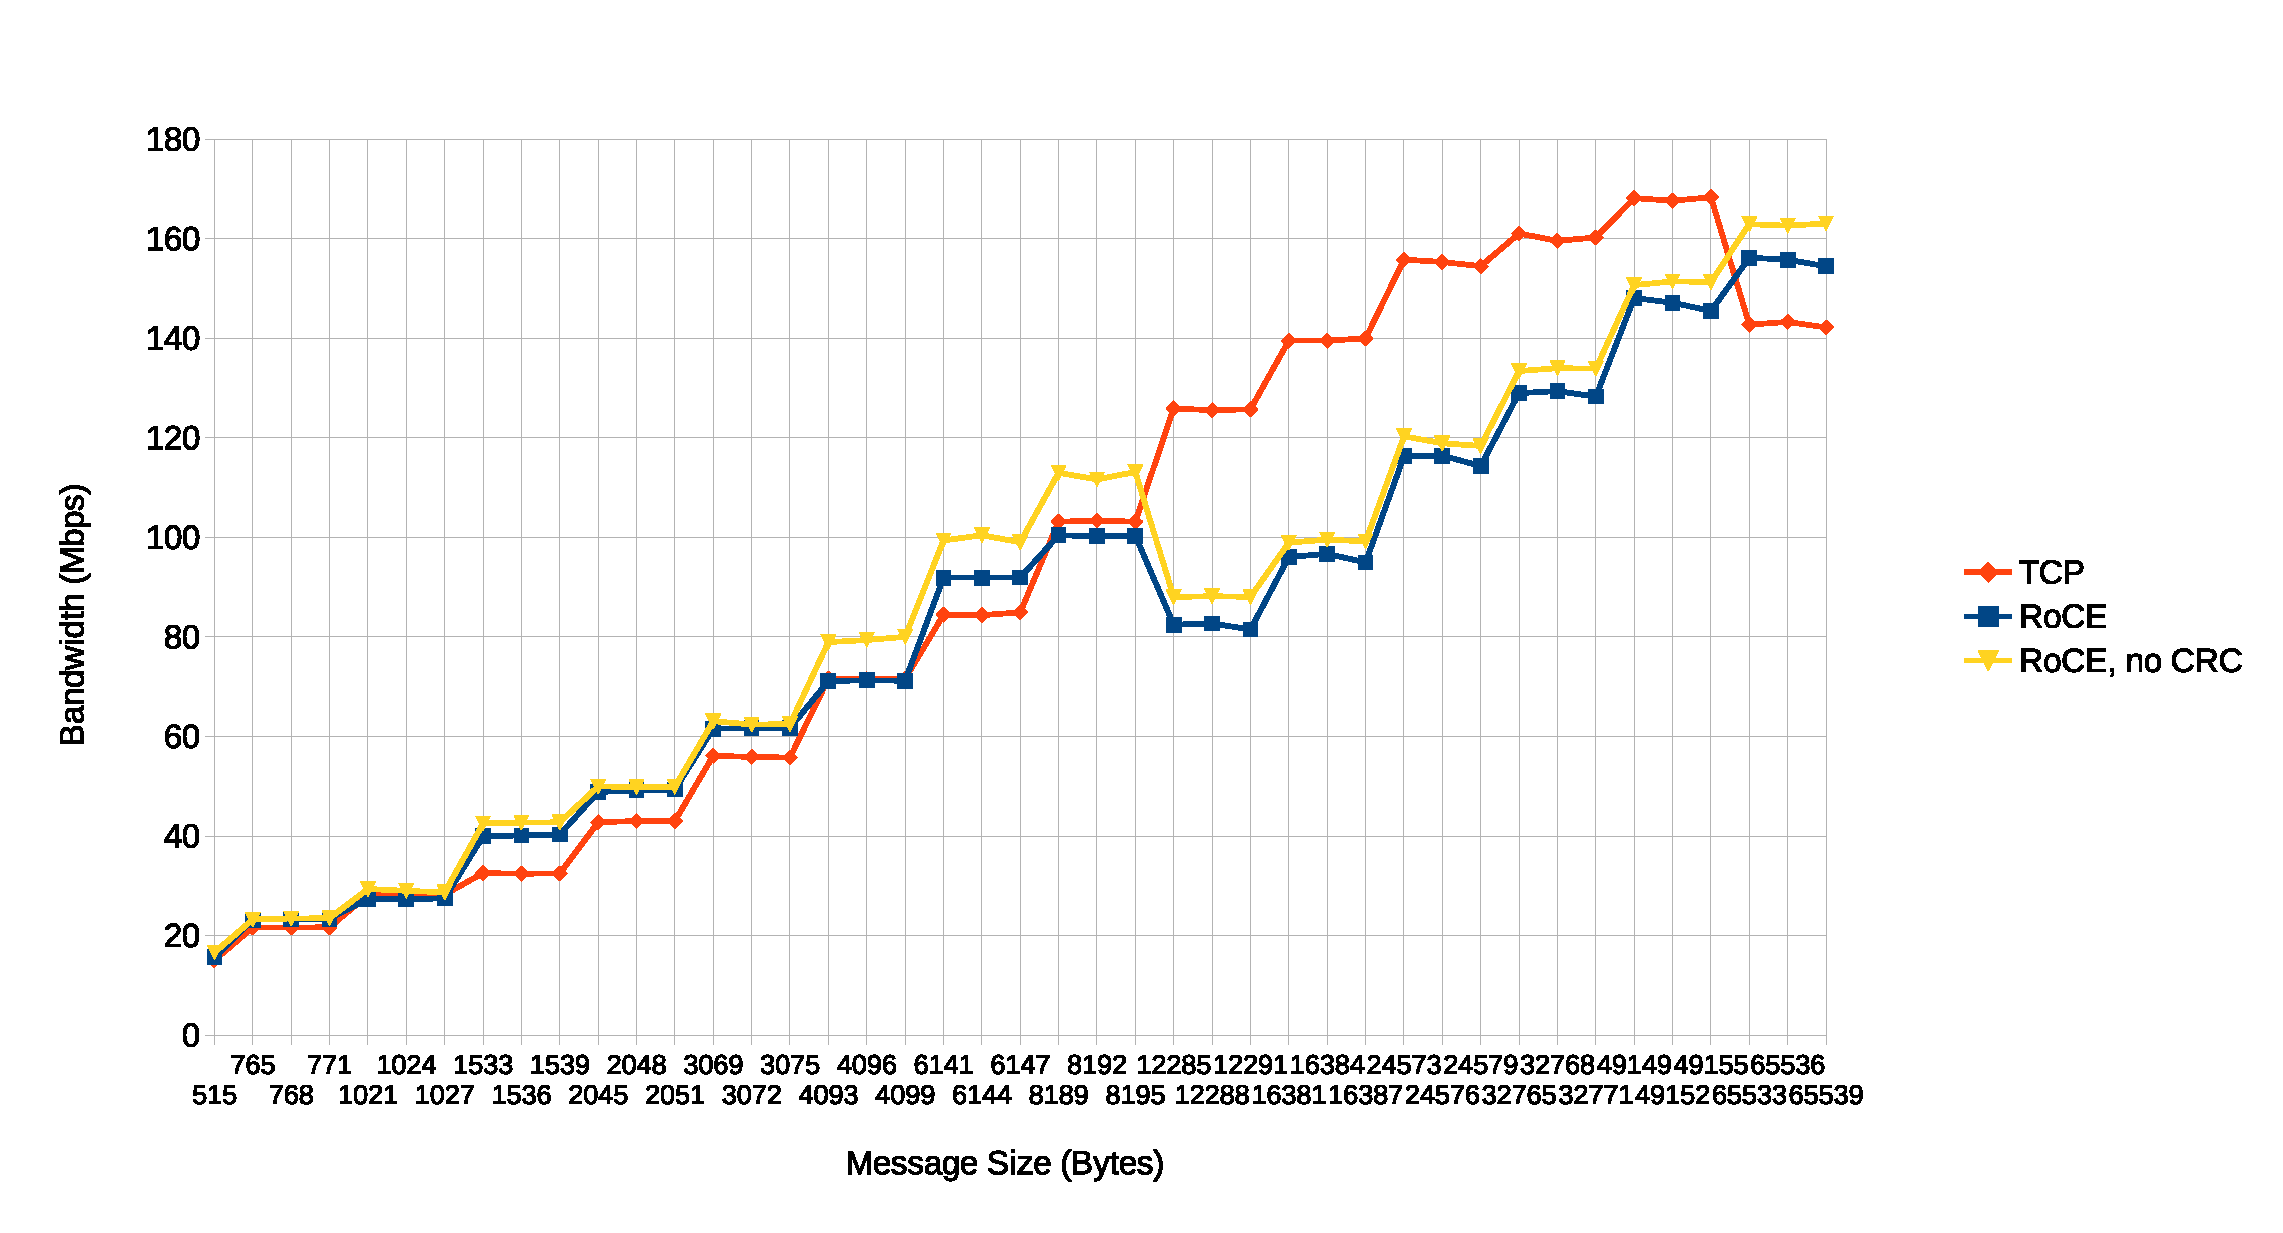
\includegraphics[width=\textwidth]{xu_bw_large}
\caption{XU NetPIPE MPI Bandwidth Results, Large Mesage Sizes}
\label{xu-bw-large}
\end{figure}

Again, the bandwidth results shown in \textbf{Figures \ref{xu-bw-small}} and
\textbf{\ref{xu-bw-large}} mirror the latency results from the same benchmarking
tool. This time, however, the maximum bandwidth is dramatically increased thanks
to the Gigabit Ethernet adaptors. However, it still does not approach the
Gigabit level. Now that we have observed this behavior from two different
USB-to-ethernet controllers, we must conclude that this is a limitation inherent
to such an architecture.

\begin{figure}[h]
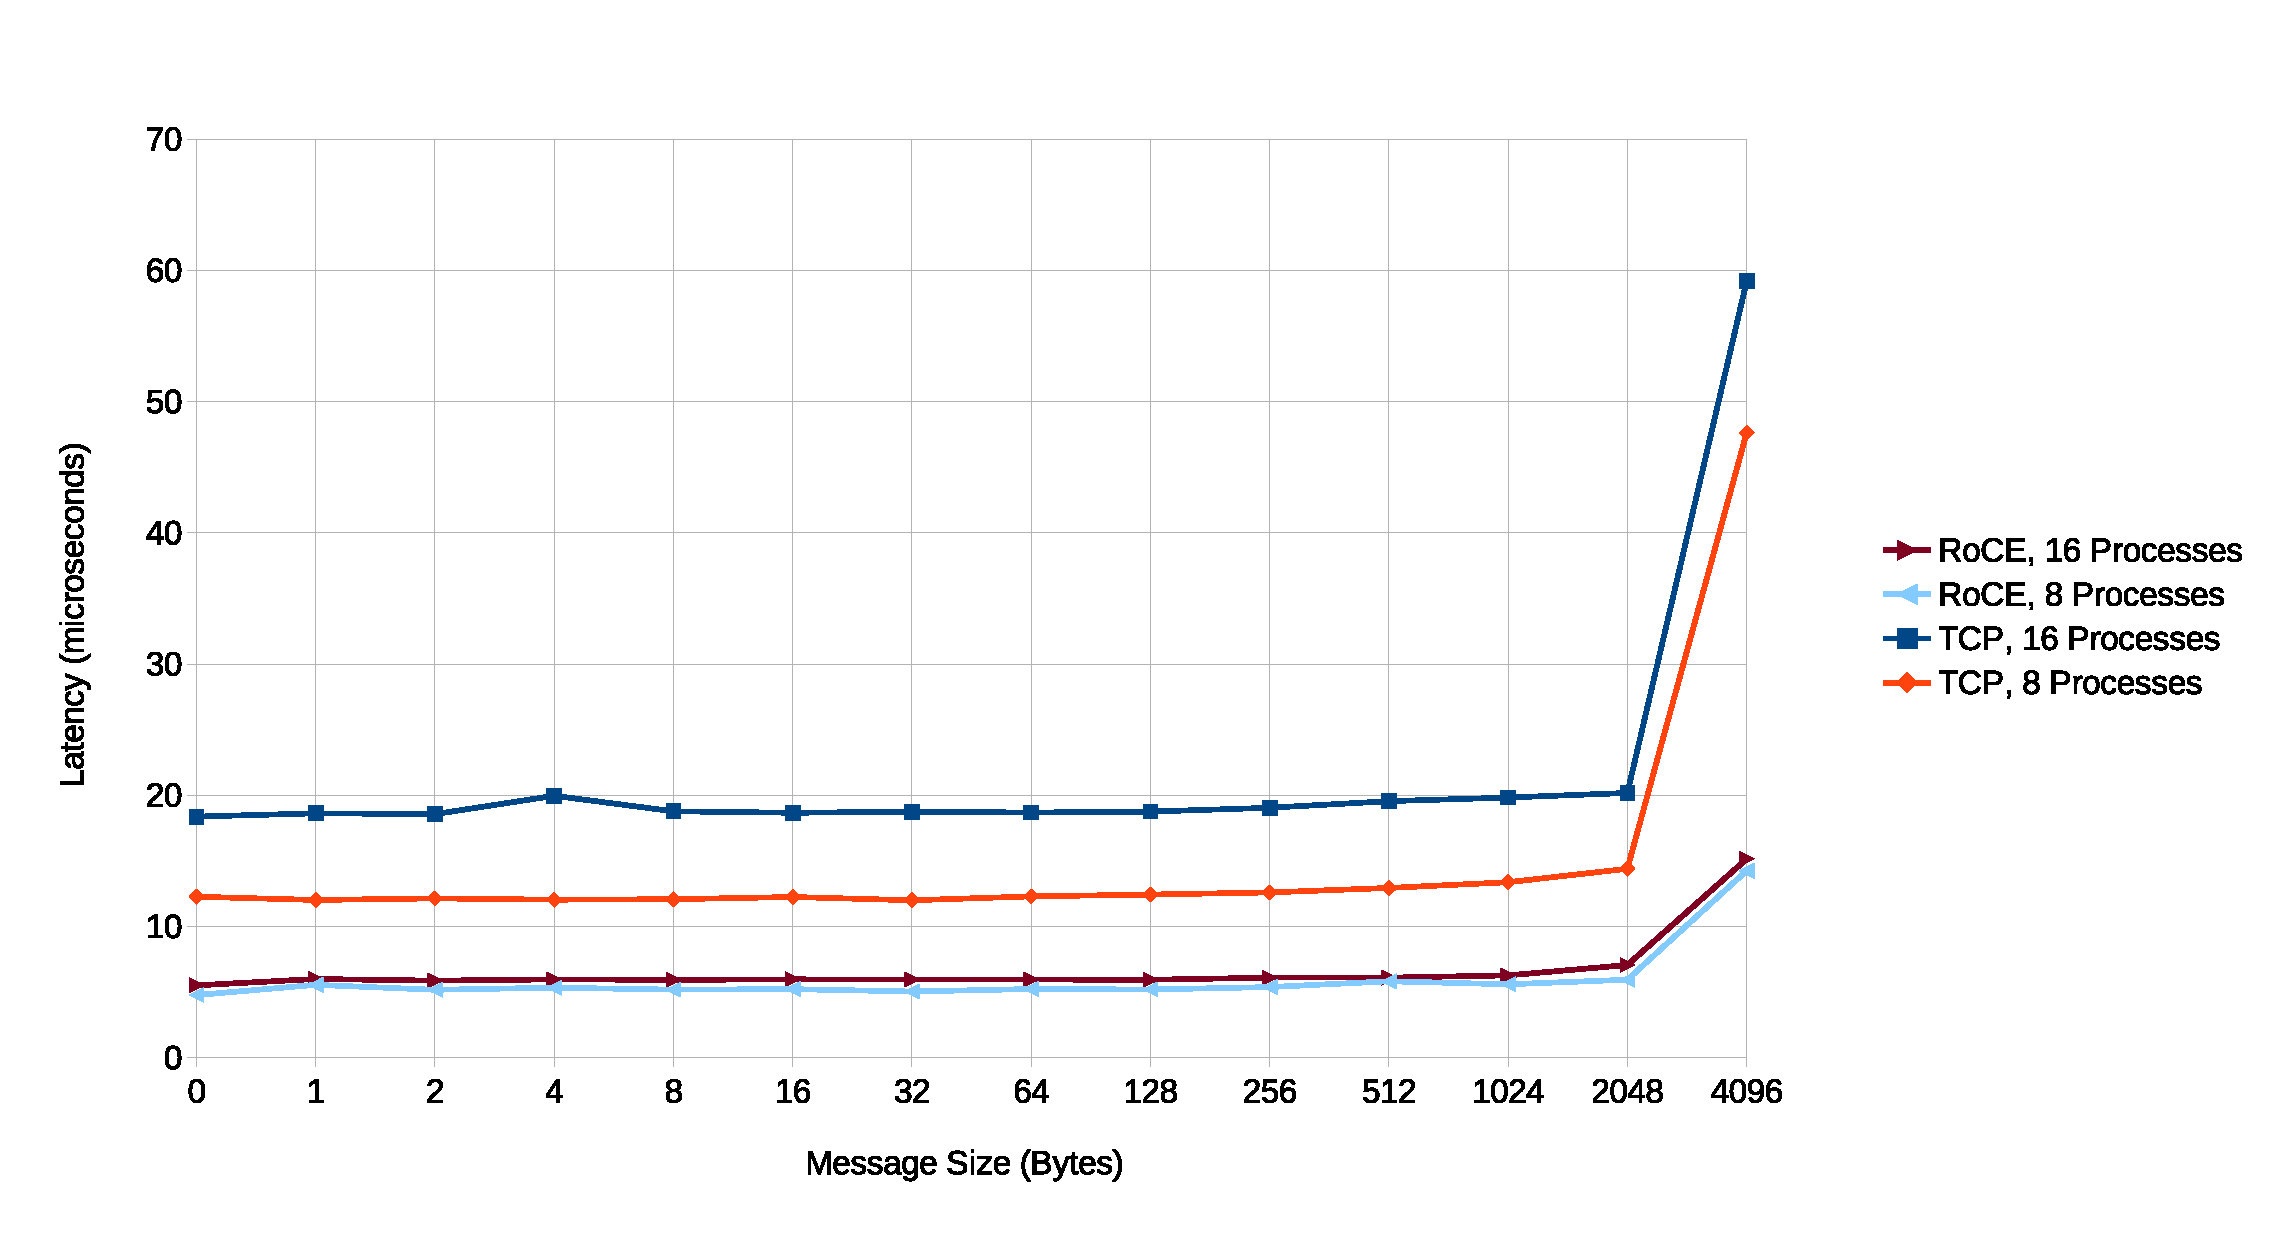
\includegraphics[width=\textwidth]{xu_imb}
\caption{Scaling of XU Message Latency with Communication Congestion}
\label{xu-imb-low}
\end{figure}

\textbf{Figure \ref{xu-imb-low}} shows the scaling of inter-process
communication latency with increased network communication. This time, we use
all four nodes in the cluster for this benchmark in order to better simulate the
communication conditions of large PDES simulations. We observe that the Exynos
5410 has drastically lower inter-process communication latency compared to the
Exynos 4412. However, this serves to highlight the lightweight characteristics
of the RoCE transport even more; up to a 3.34 times speedup is possible for very
small messages when all cores are utilized. Even when only two of four cores are
in use, 2.5 times speedup is possible.

\section{\textbf{PDES Results}}
\label{pdes-results}

\href{https://github.com/carothersc/ROSS}{Rensselaer's Optimistic Simulation
  System (ROSS)} is used for all PDES experiments. It uses MPI for all
inter-process communication, including local communication
\cite{carothers-02}. Its optimistic synchronization protocol uses the Time Warp
paradigm with some modifications. Notably, ROSS features the addition of Kernel
Processes (KPs) that aggregate processed event lists and perform all the
rollback computations, while the traditional LPs perform forward computation
\cite{carothers-02}. There must be at least one LP assigned to each KP, but
assigning several LPs to each KP can reduce memory footprint for many
simulations \cite{carothers-02}.

For the results shown in this section, we use three of the simulation models
included with ROSS: \verb;wifi;, \verb;disksim;, and \verb;raid;. The number of
LPs used for each model is tuned so that startup overhead is not a significant
portion of simulation runtime but memory is not exhausted. As the number of
processes used in the simulation is varied, the number of LPs remains the same,
although the number of KPs changes as it remains at the default allocation per
process. \textbf{Table \ref{lptable}} lists the total number of LPs across all
processes as well as the termination time set for each model. This configuration
is used for both the ARM and x86 clusters in order to allow a direct performance
comparison.

\begin{table}
  \caption{ROSS Simulation Model Parameters}
  \label{lptable}
  \centering
  \begin{tabular}[c]{| l | r | r | r |}
    \hline
    Model Name & LPs & Memory per Node (MB) & Temination Time (GVT) \\ \hline
    \textsc{disksim} & 768 & 1536 & 10000000 \\
    \textsc{raid} & 384 & 1536 & 10000 \\
    \textsc{wifi} & 96 & 1536 & 10000 \\
    \hline
  \end{tabular}
\end{table}

Simulation runtime results as reported by ROSS are shown throughout the rest of
this section. For each model, results from the x86 cluster and results from the
ARM cluster over TCP and over RoCE are presented. The error bars in
\textbf{Figures \ref{disksim}, \ref{raid},} and \textbf{\ref{wifi}} show a 99\%
confidence interval for the mean simulation time.

\begin{figure}
\centering
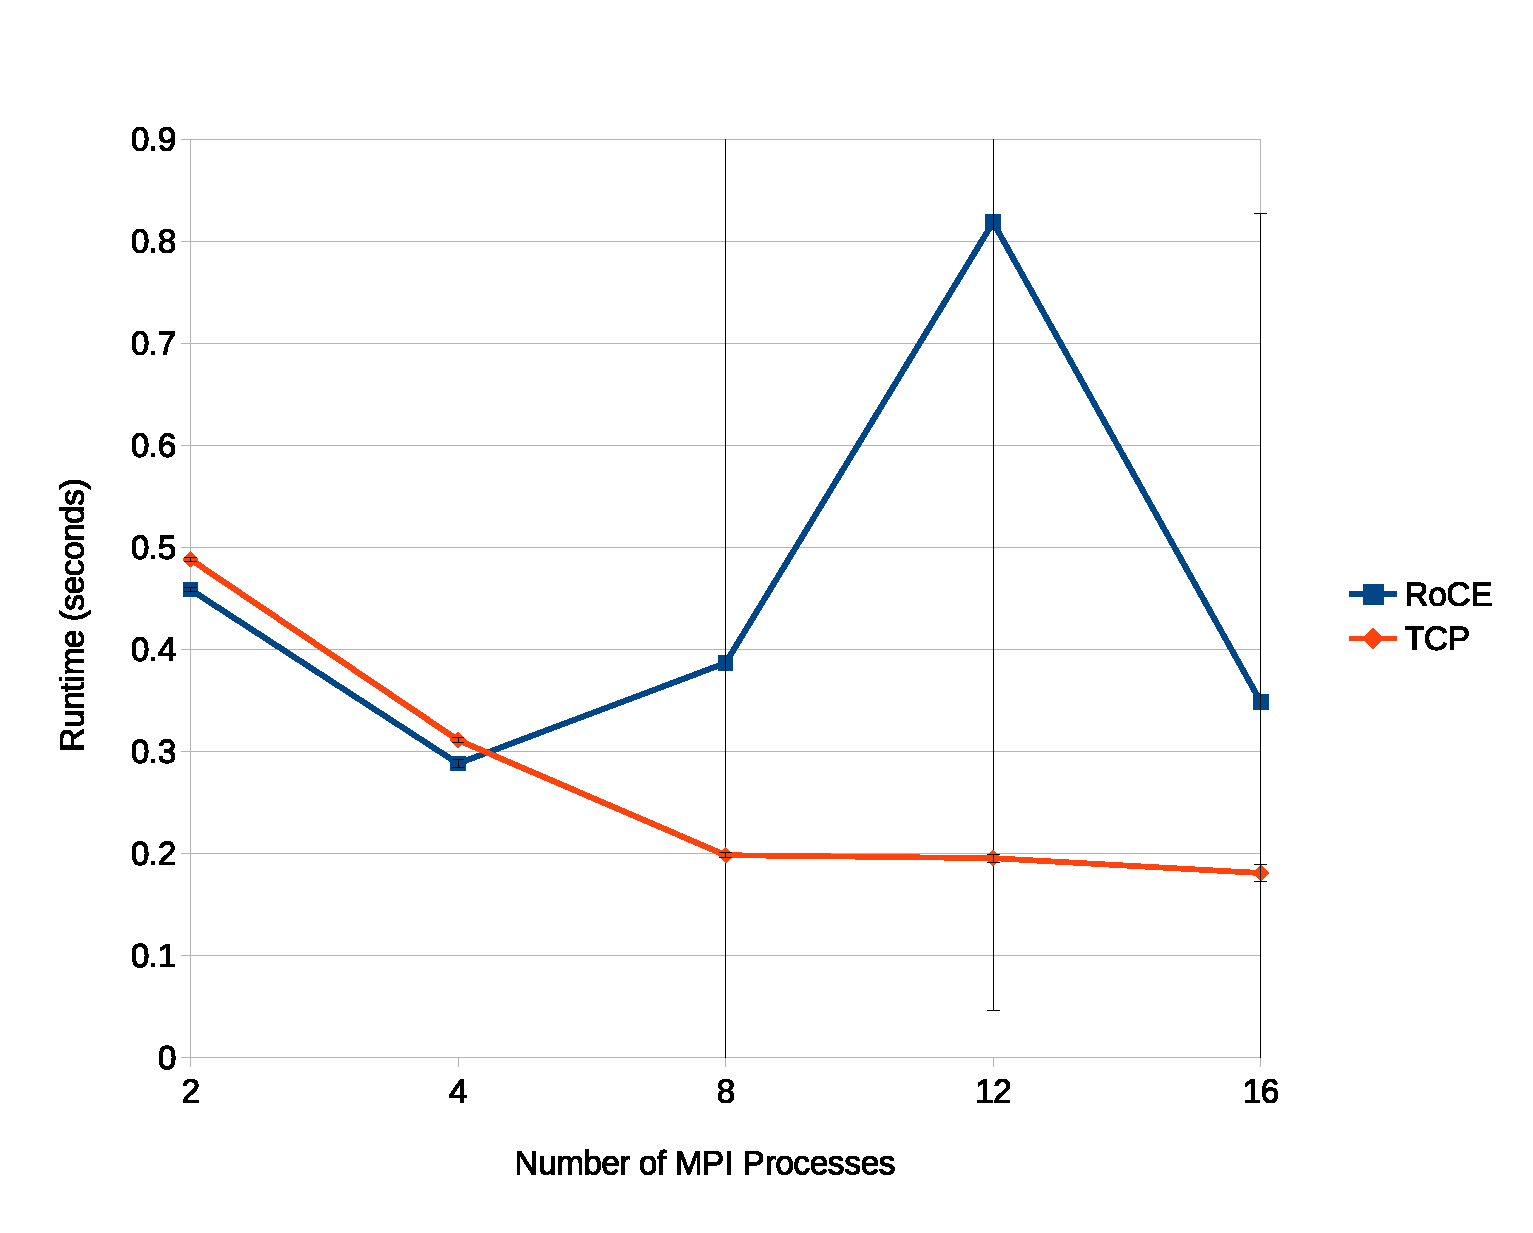
\includegraphics[width=0.75\textwidth]{disksim}
\caption{Mean Simulation Runtimes for ROSS \textsc{disksim} Model}
\label{disksim}
\end{figure}

\begin{figure}
\centering
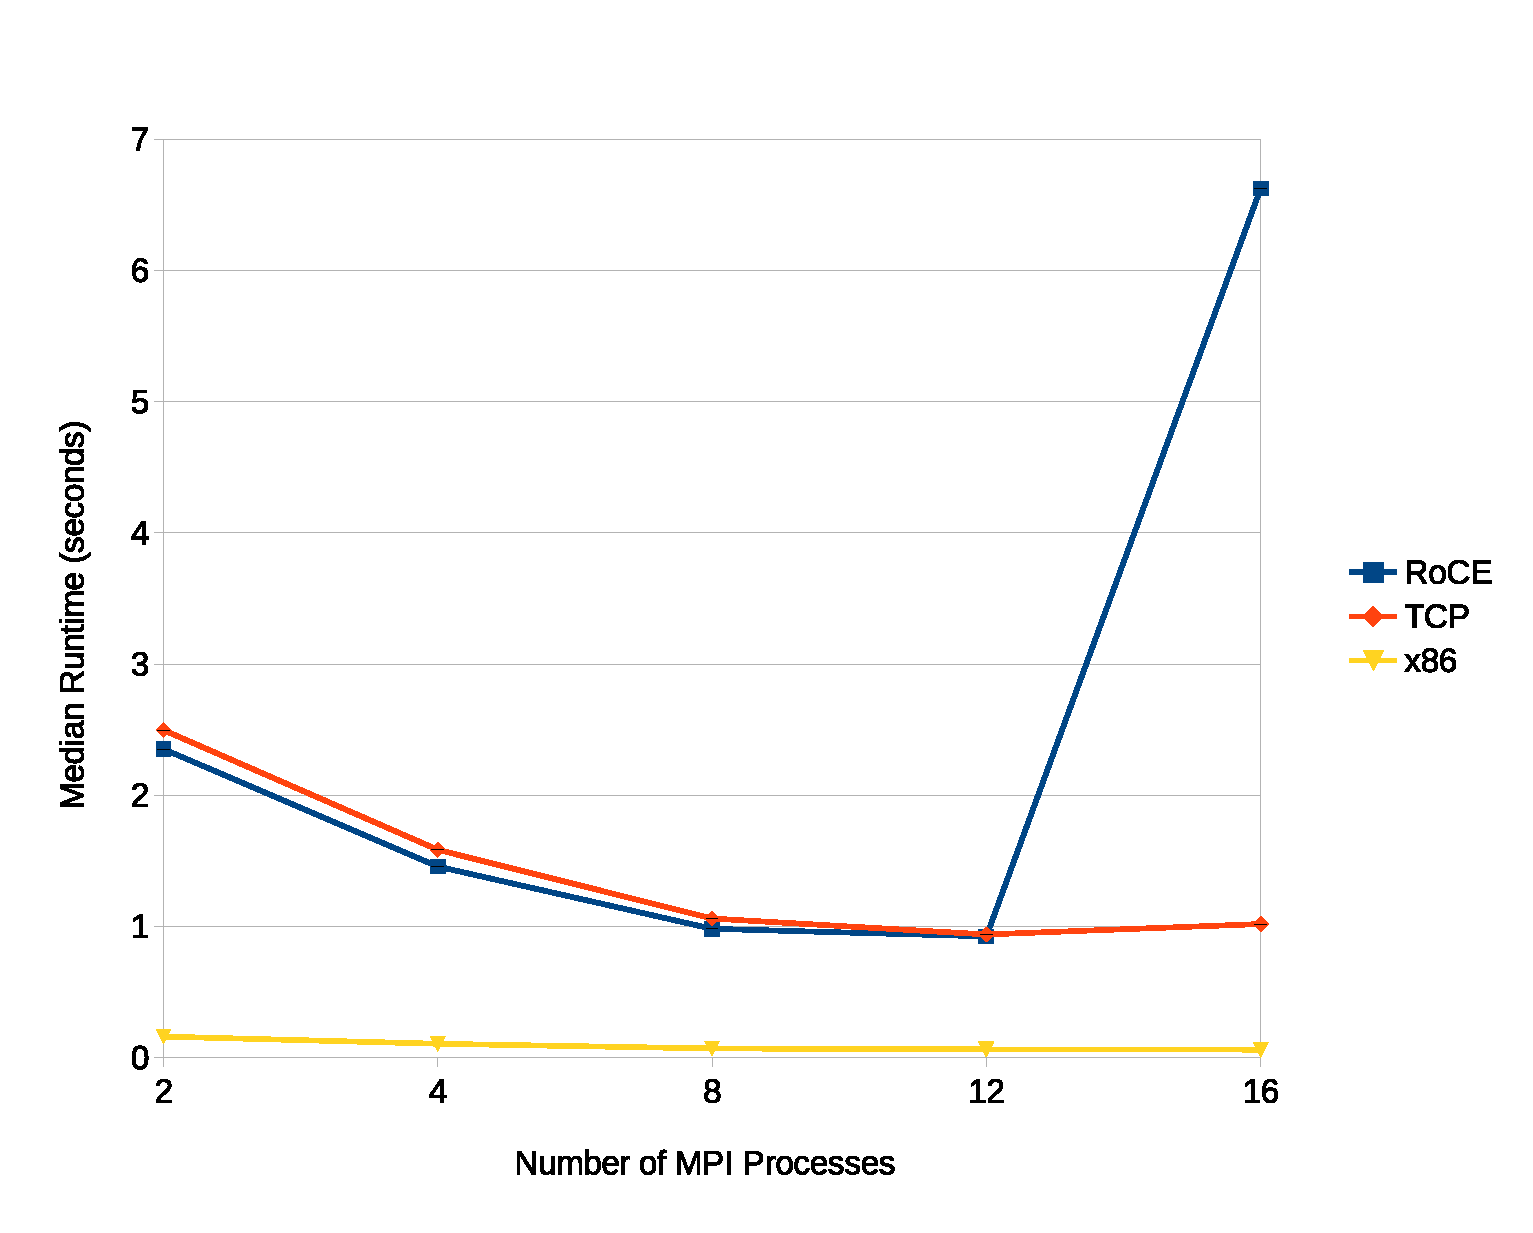
\includegraphics[width=0.75\textwidth]{disksim_median}
\caption{Median Simulation Runtimes for ROSS \textsc{disksim} Model}
\label{disksim-median}
\end{figure}

The \verb;disksim; model is an example of a small model that we can run with a
high number of LPs. We can see from \textbf{Figure \ref{disksim}} that RoCE
slightly improves runtime over TCP when no more than one MPI process is
allocated to the node. When two or more MPI processes are allocated per compute
node, the runtimes become unstable, occasionally stalling for many times the
average runtime. For comparison, \textbf{Figure \ref{disksim-median}} shows the
median simulation runtimes for the same set of tests. Aside from the stalls, it
is clear that the performance of RoCE is a constant factor better than TCP for 8
and 16 total MPI processes as well as 2 and 4.

\begin{figure}
\centering
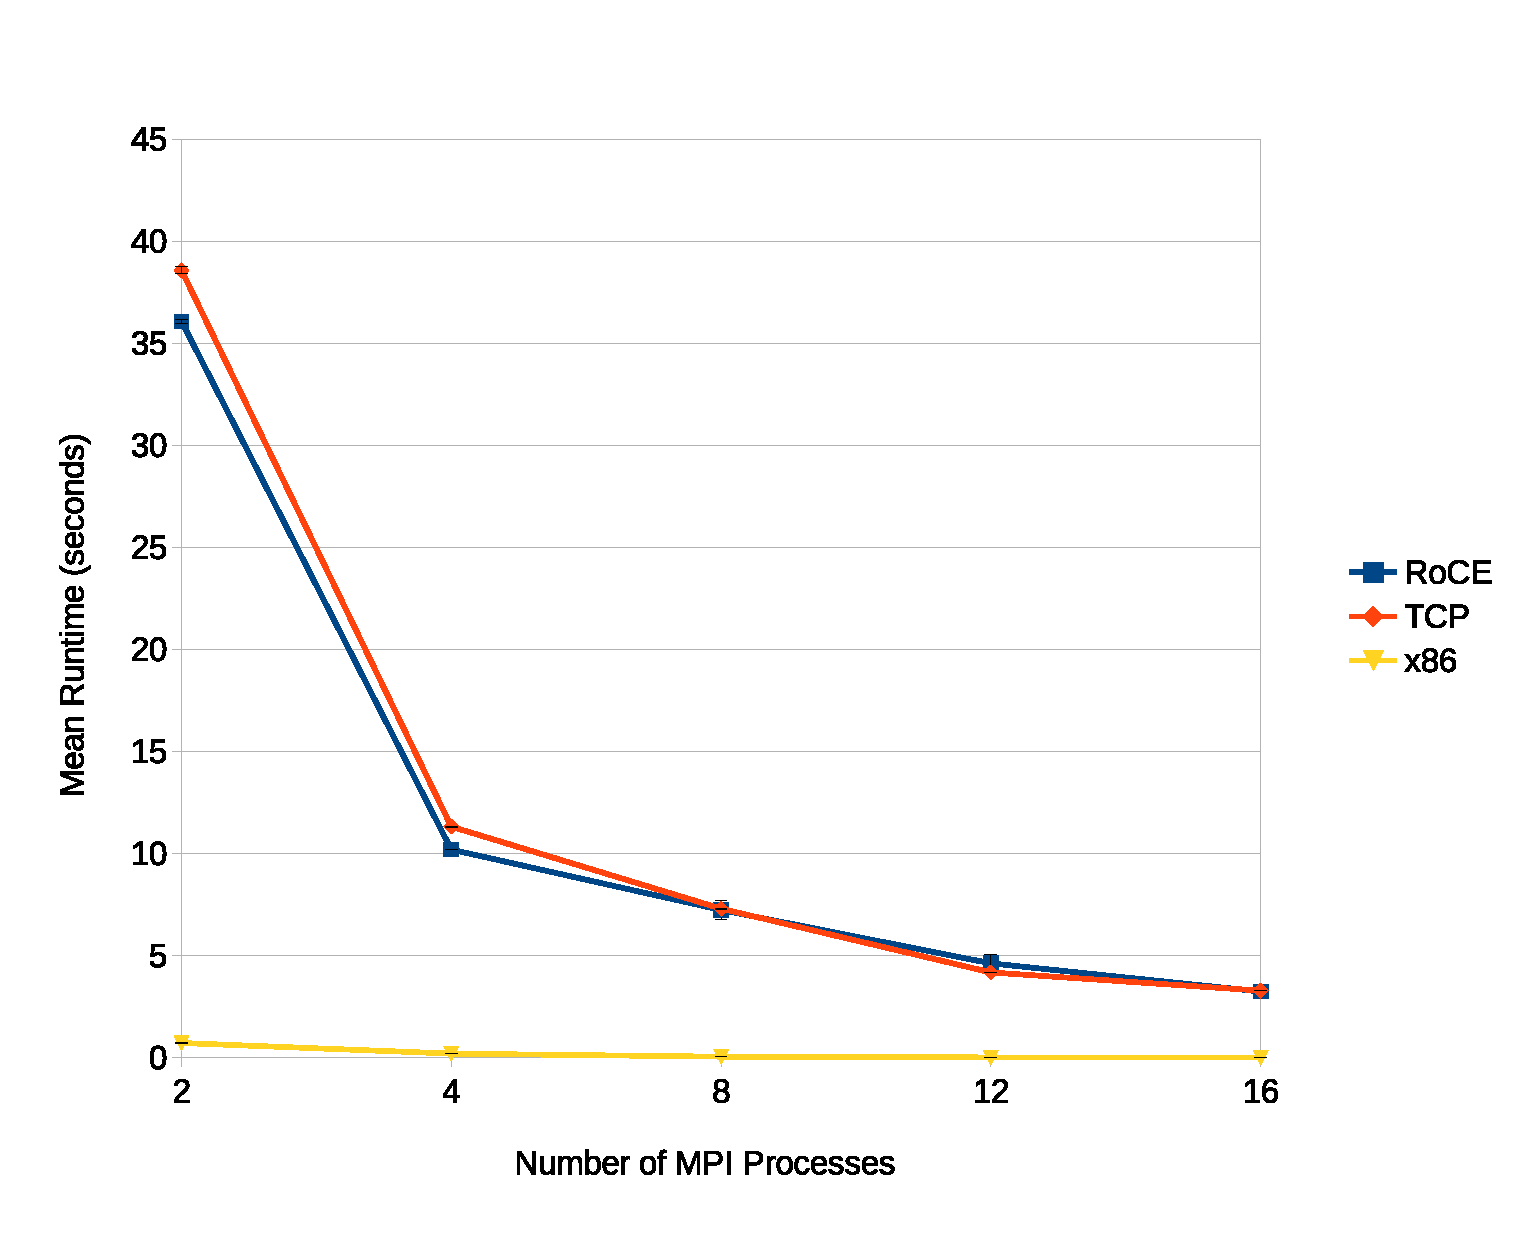
\includegraphics[width=0.75\textwidth]{raid}
\caption{Mean Simulation Runtimes for ROSS \textsc{raid} Model}
\label{raid}
\end{figure}

\begin{figure}
\centering
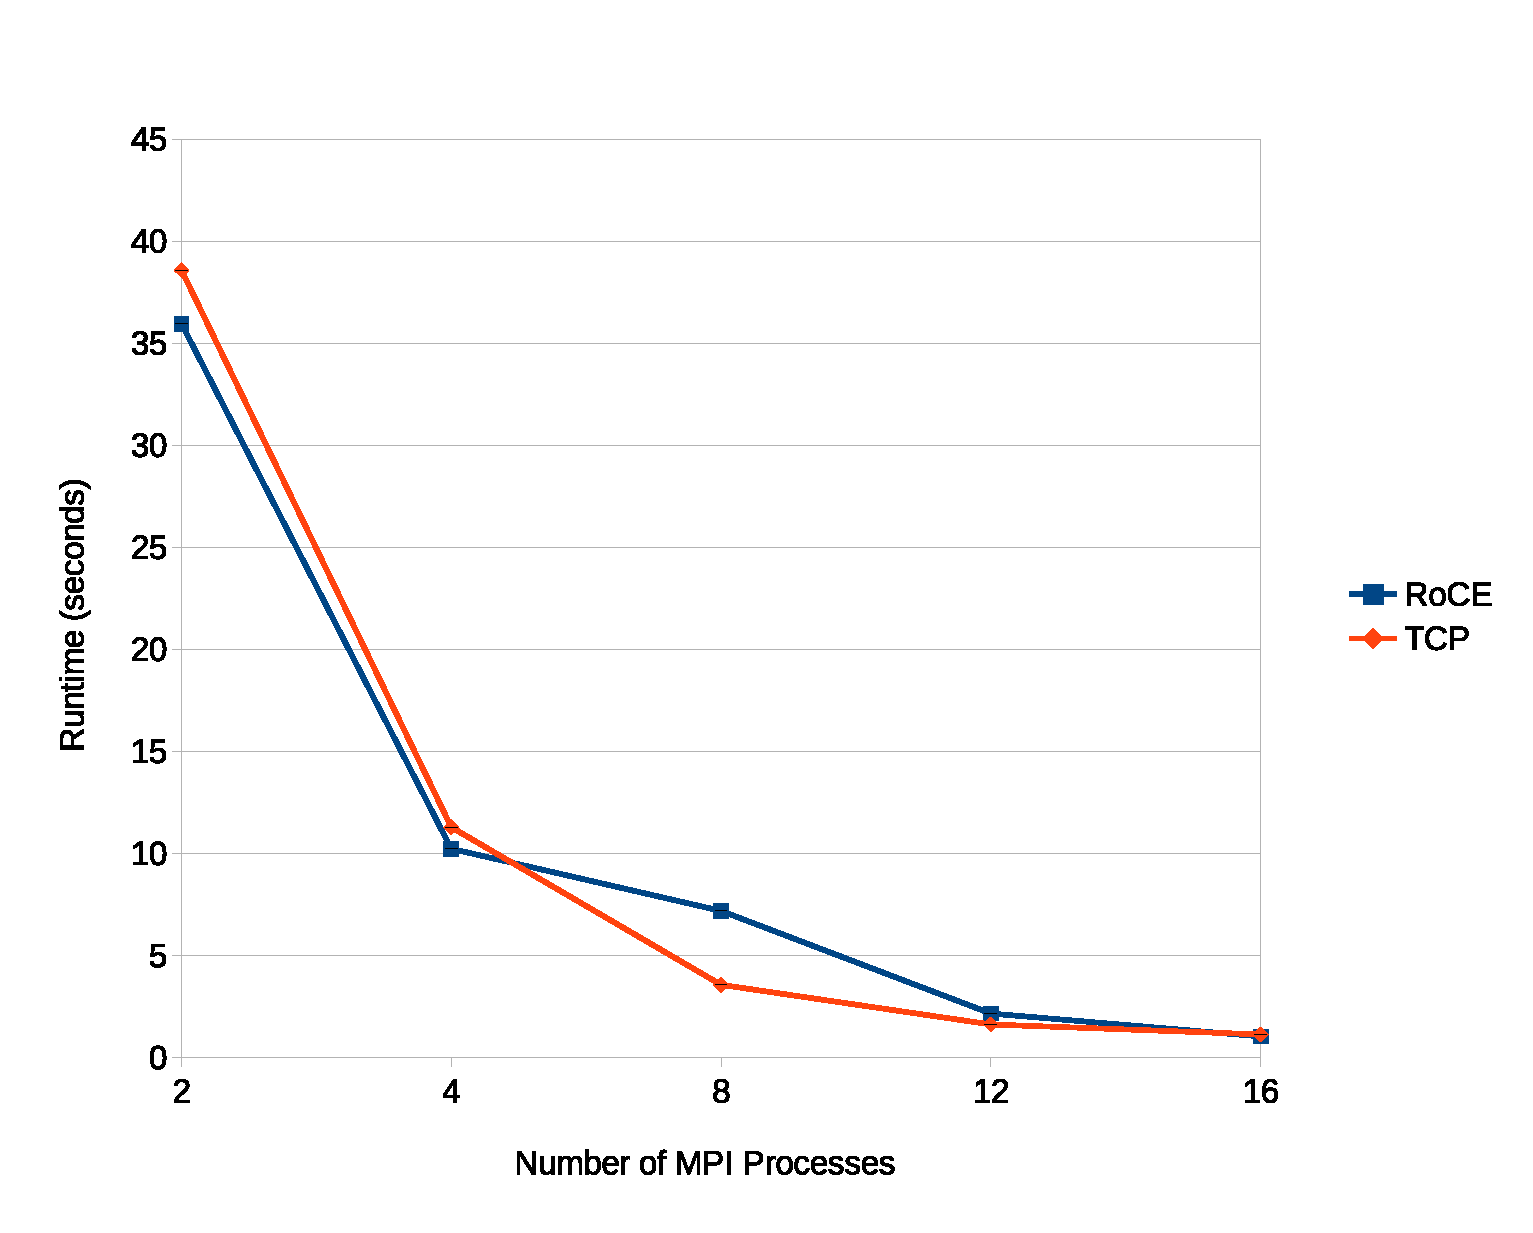
\includegraphics[width=0.75\textwidth]{raid_median}
\caption{Median Simulation Runtimes for ROSS \textsc{raid} Model}
\label{raid-median}
\end{figure}

We can observe nearly the same phenomenon from tests using the \verb;raid;
model, the results of which are shown in \textbf{Figures \ref{raid}} and
\textbf{\ref{raid-median}}. This time, our confidence interval is sufficiently
small to conclude that RoCE performs worse than TCP when more than one MPI
process is allocated per node. This is in stark contrast to the predictions of
the micro-benchmark results from \textbf{Section
  \ref{final-cluster-benchmarks}}, especially those that measure the scaling of
inter-process communication latency. A possible explanation for these PDES
results in light of the micro-benchmark results is that the factor difference
between the latency of shared memory communication compared to remote node
communication is greater for RoCE than TCP. In fact, the factor difference is
more than double according to \textbf{Figure \ref{xu-imb-low}}.

\begin{figure}
\centering
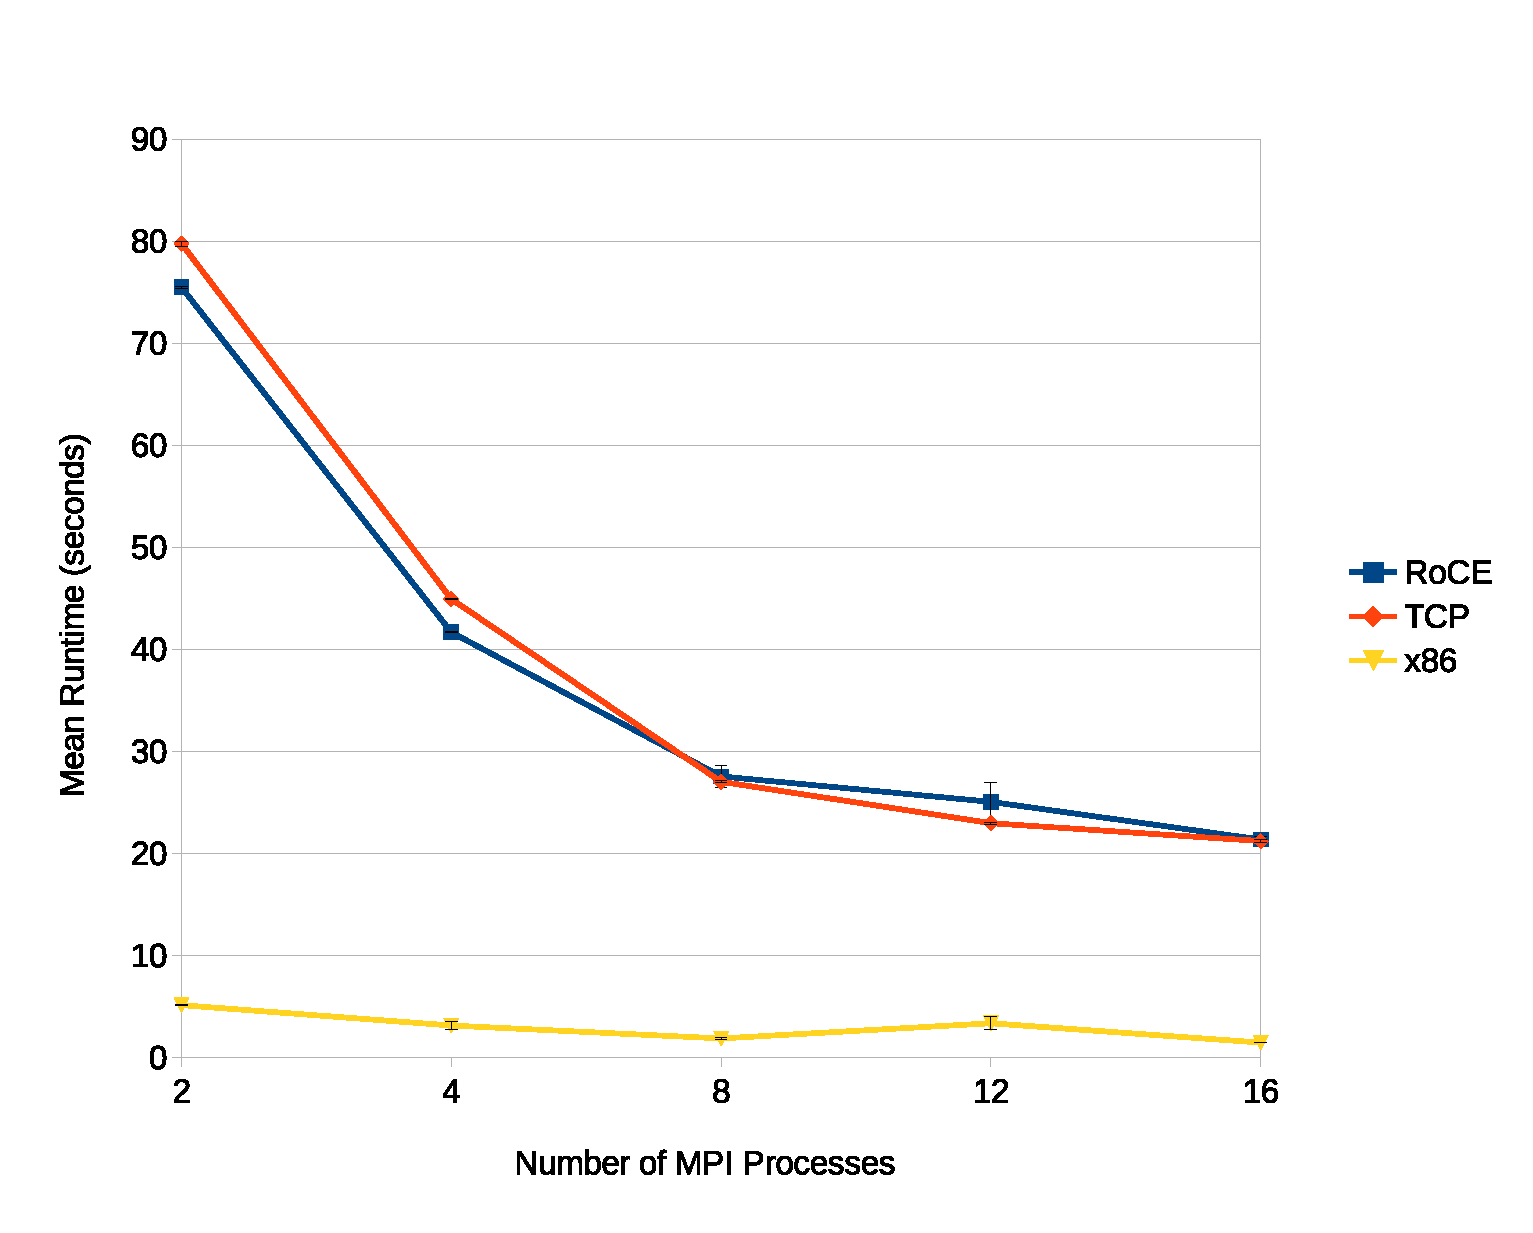
\includegraphics[width=0.75\textwidth]{wifi}
\caption{Mean Simulation Runtimes for ROSS \textsc{wifi} Model}
\label{wifi}
\end{figure}

\begin{figure}
\centering
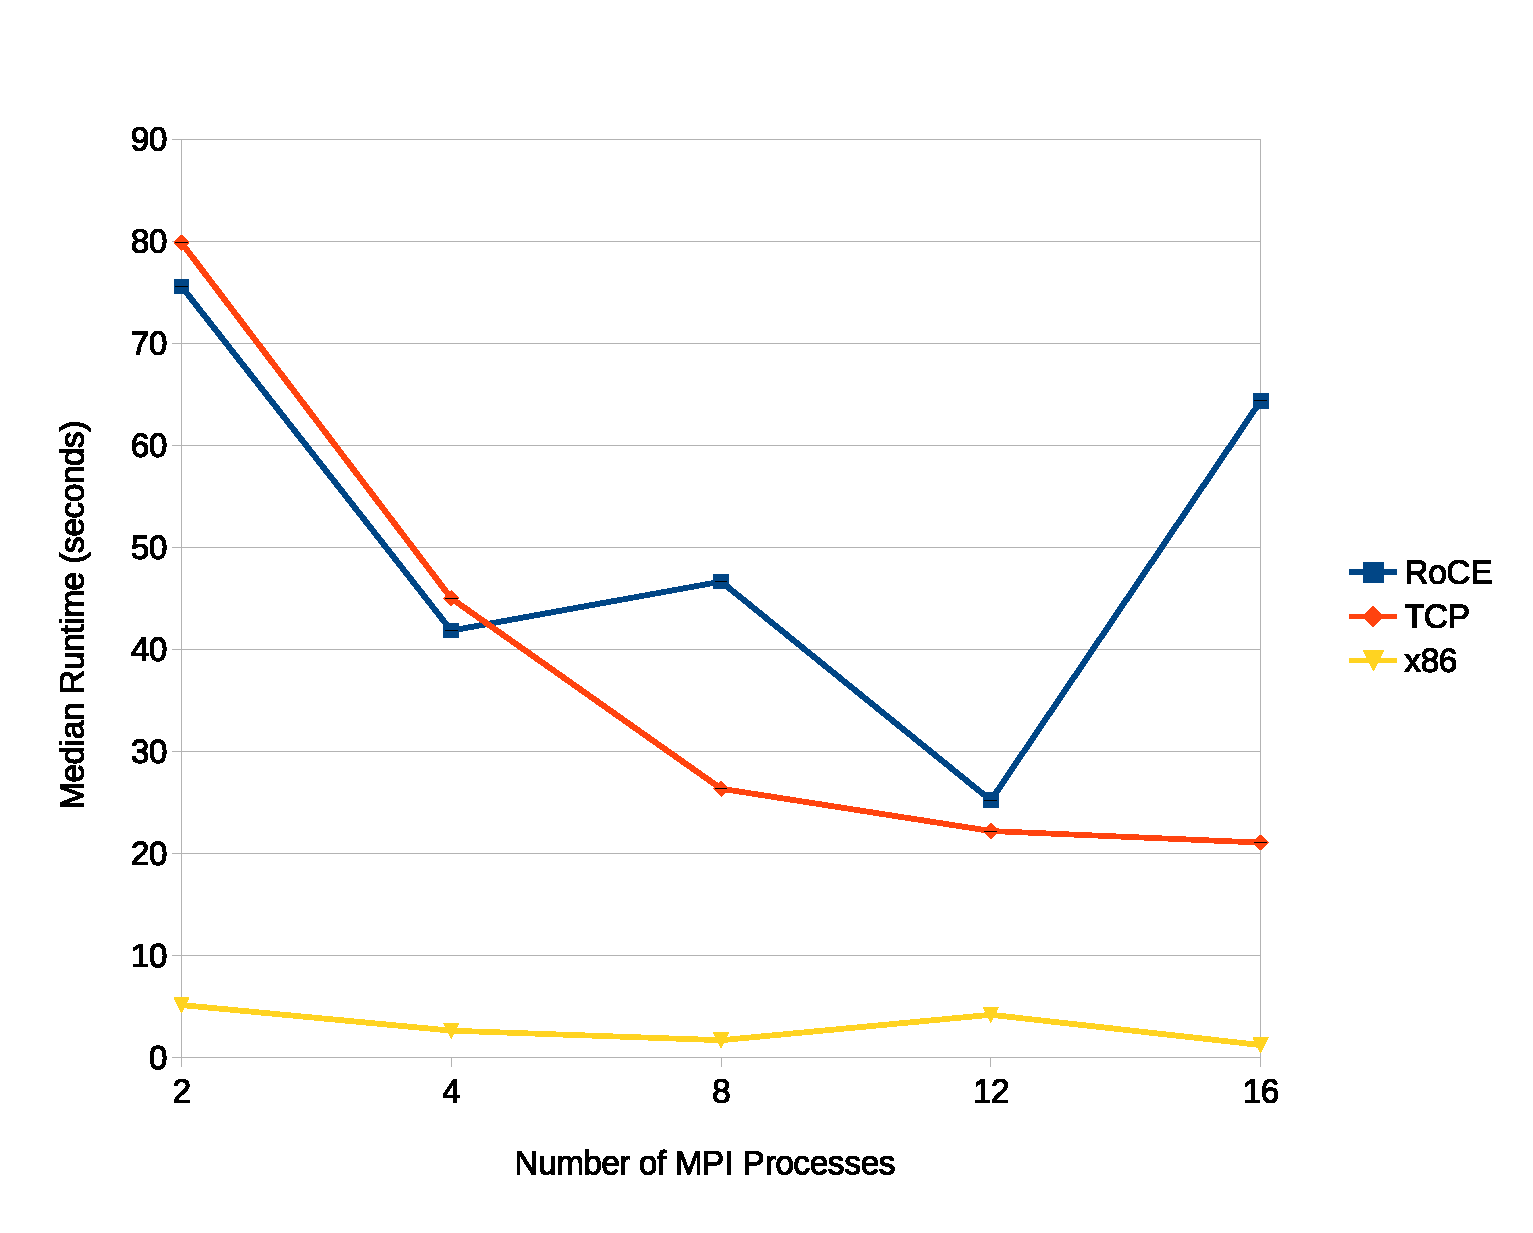
\includegraphics[width=0.75\textwidth]{wifi_median}
\caption{Median Simulation Runtimes for ROSS \textsc{wifi} Model}
\label{wifi-median}
\end{figure}

Finally, the \verb;wifi; model results in \textbf{Figures \ref{wifi}} and
\textbf{\ref{wifi-median}} show the same problem without the large variance seen
in the \verb;disksim; and \verb;raid; models. Clearly, network message latency
alone is not a good predictor for PDES performance when more than one
communication layer is in use.


\subsection{\textbf{RoCE Speedup}}

\textbf{Figures \ref{disksim-speedup}, \ref{raid-speedup},} and
\textbf{\ref{wifi-speedup}} show the mean speedup obtained by using the RoCE
transport compared to TCP on the ARM cluster. Speedup is defined as
$\frac{runtime_{TCP}}{runtime_{RoCE}}$, so values greater than one indicate speedup,
while values less than one indicate slowdown.

For all three models, we observe a consistent speedup between 5\% and 15\% when
there is a maximum of one MPI process per node and a drastic slowdown when
at least two MPI processes are allocated per node. Again, this may indicate that
the transport is sensitive to large differences in message latency between LPs.

\begin{figure}
\centering
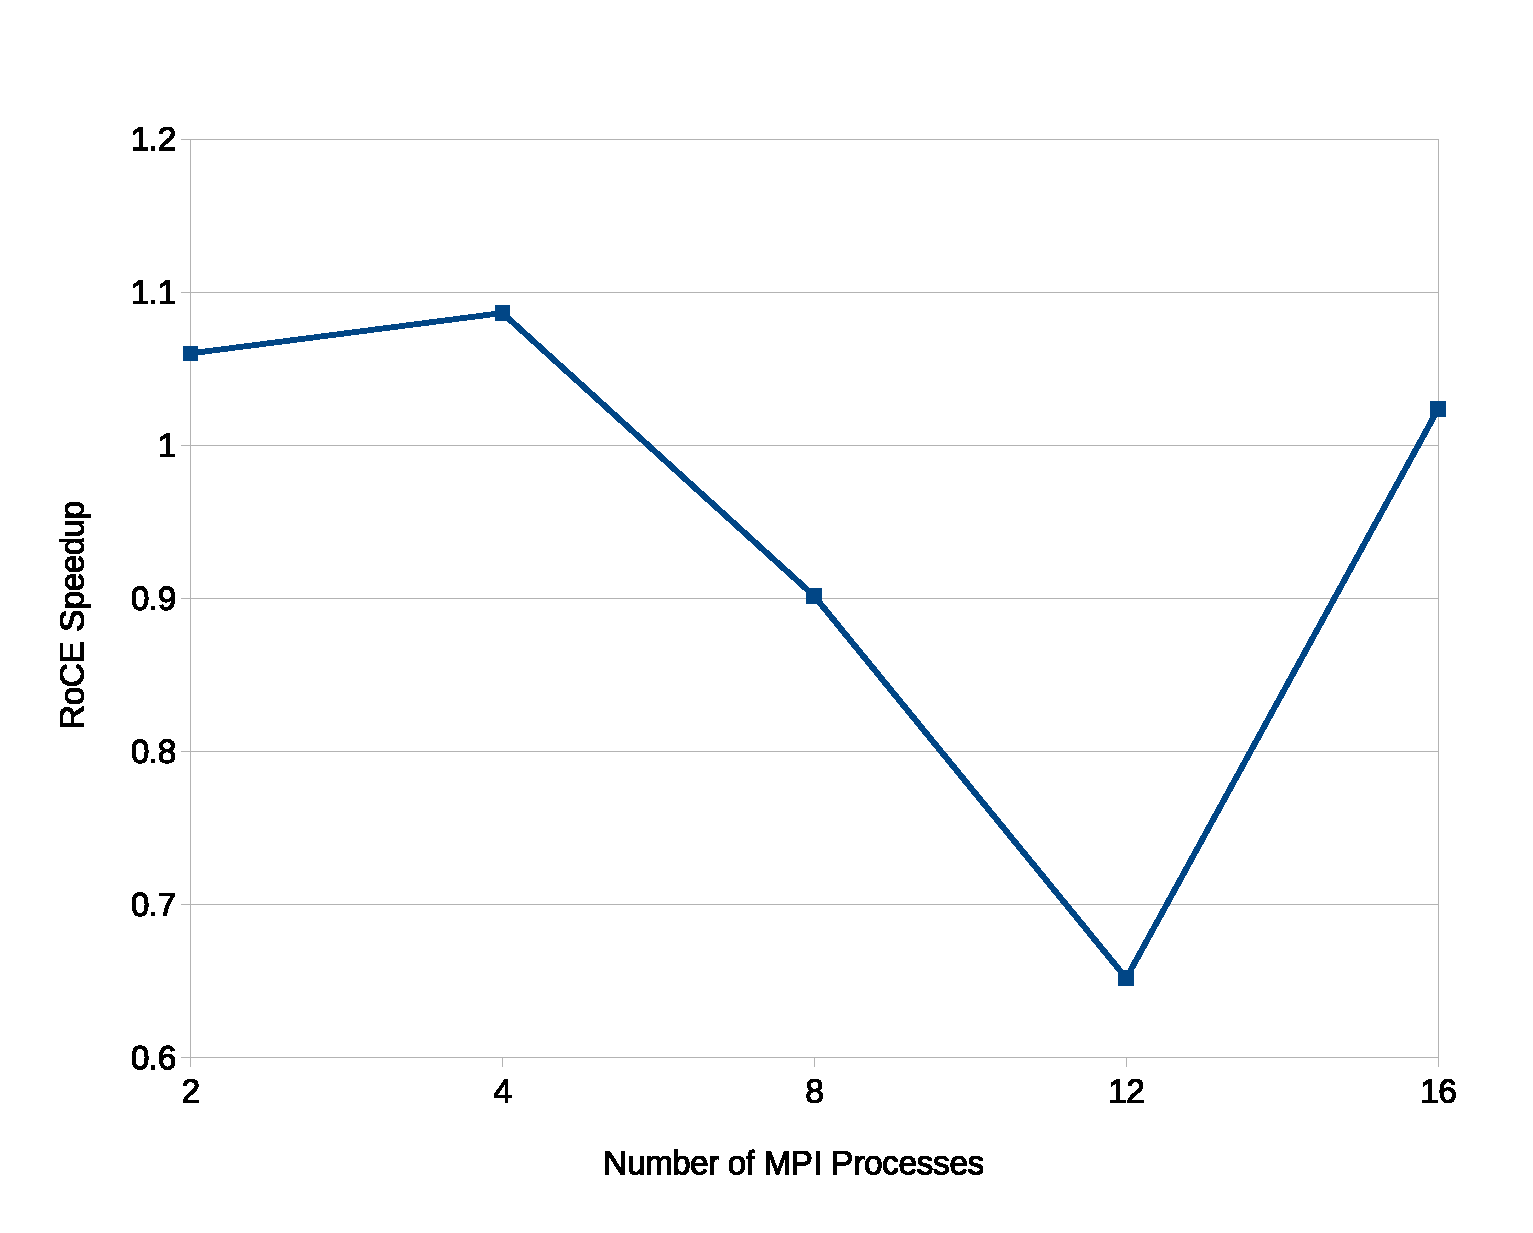
\includegraphics[width=0.75\textwidth]{disksim_speedup}
\caption{RoCE Speedup for \textsc{disksim} Model}
\label{disksim-speedup}
\end{figure}

\begin{figure}
\centering
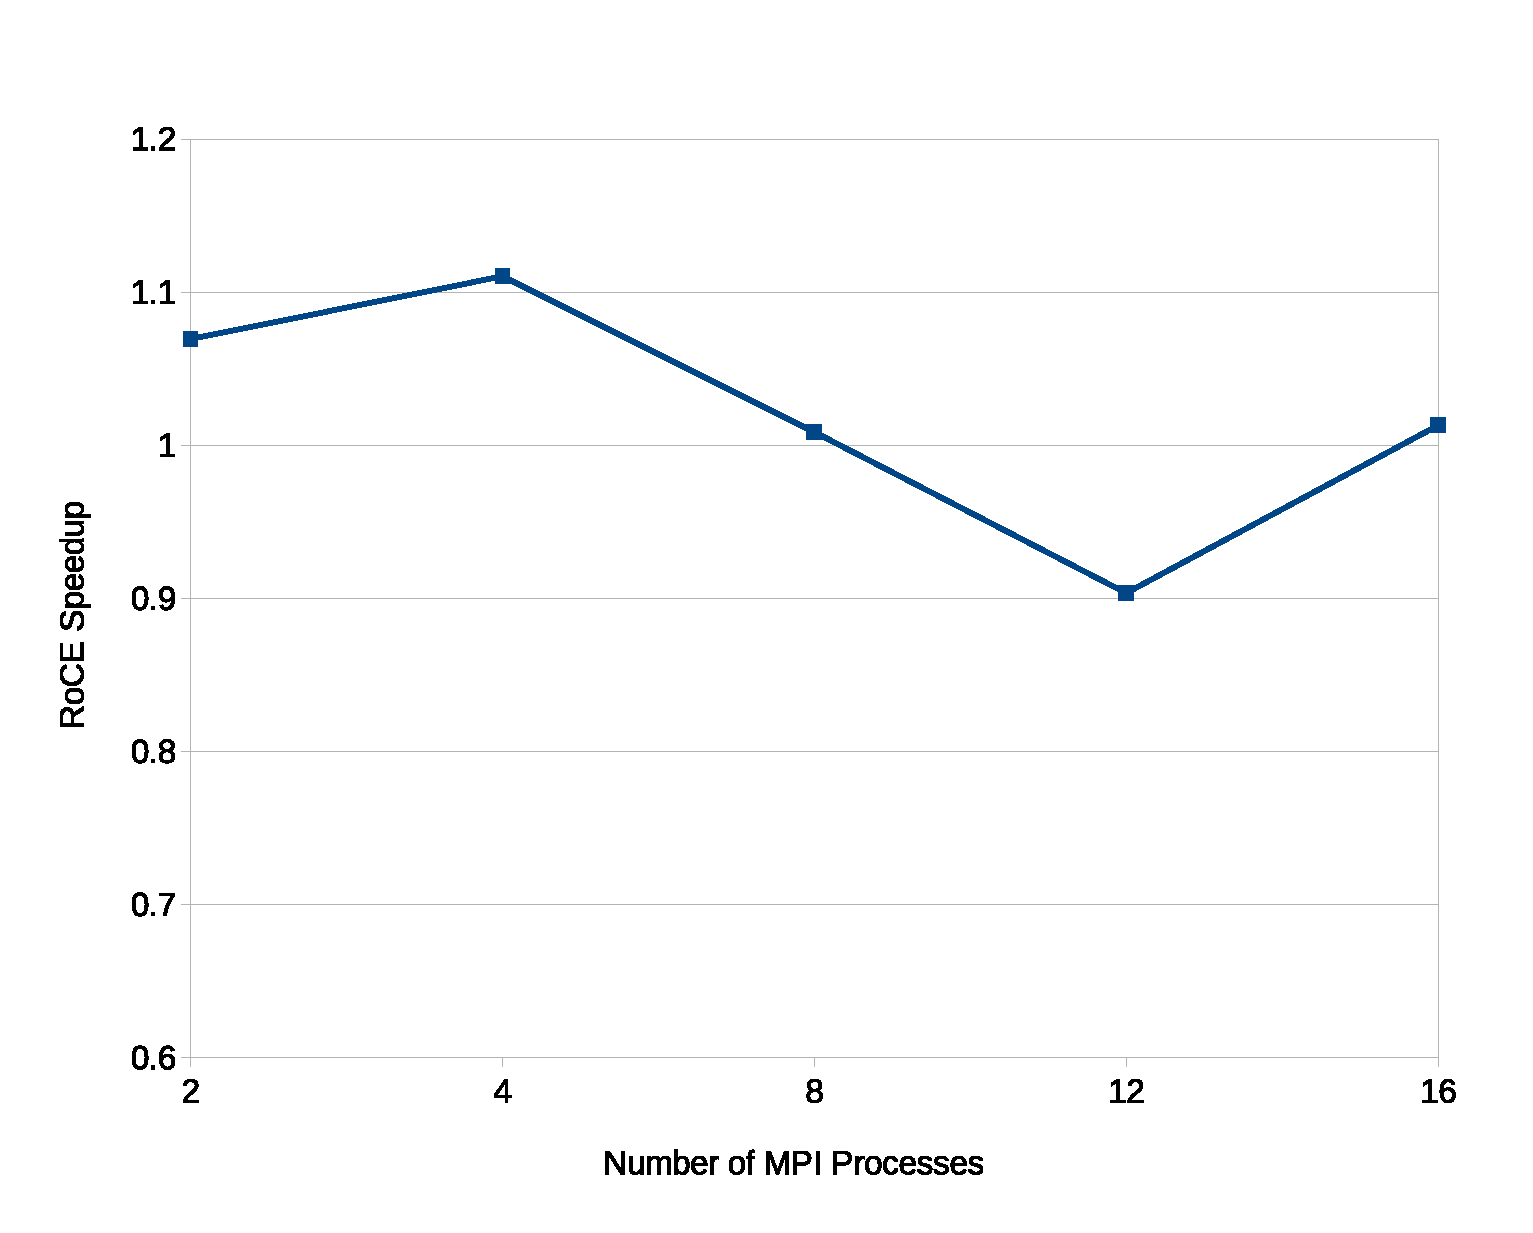
\includegraphics[width=0.75\textwidth]{raid_speedup}
\caption{RoCE Speedup for \textsc{raid} Model}
\label{raid-speedup}
\end{figure}

\begin{figure}
\centering
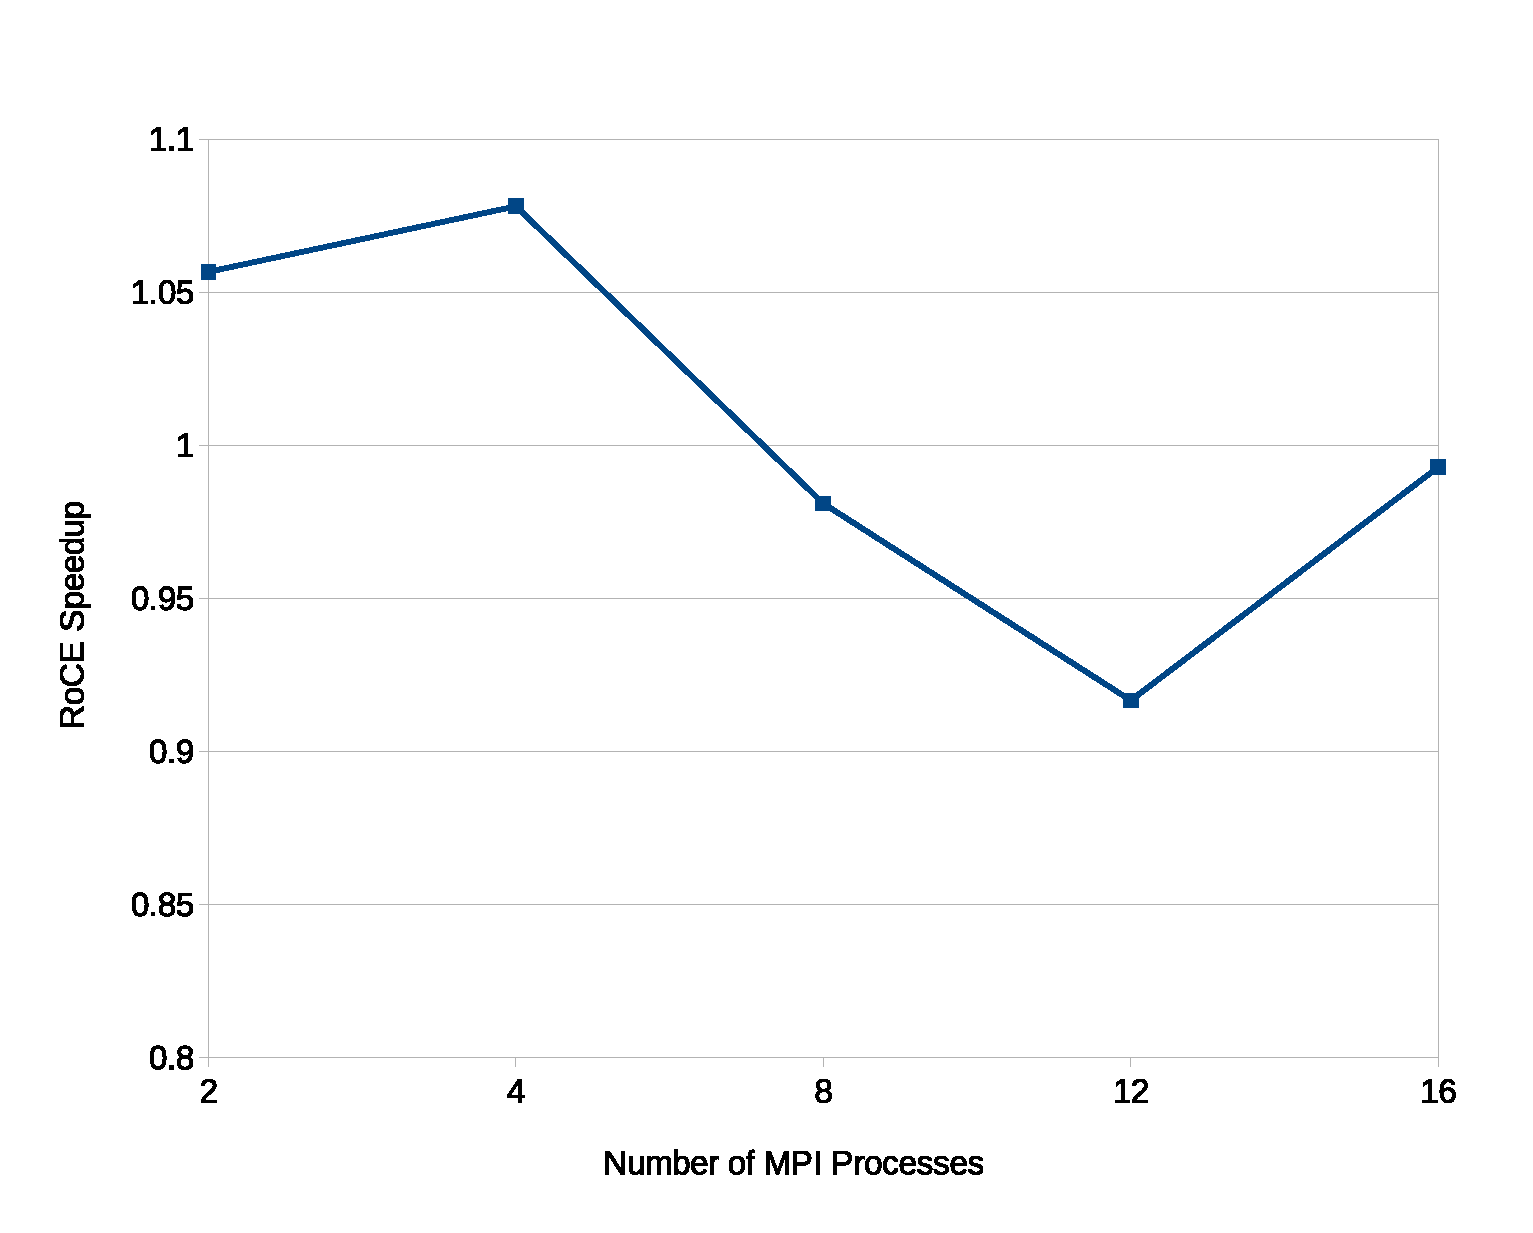
\includegraphics[width=0.75\textwidth]{wifi_speedup}
\caption{RoCE Speedup for \textsc{wifi} Model}
\label{wifi-speedup}
\end{figure}


\newpage
\chapter{Discussion}
\label{conclusions}

\section{\textbf{Cost and Performance Comparisons}}

In this section, I present performance-for-cost data calculated using the
results from \textbf{Chapter \ref{pdes-results}}. First, performance for cost is
defined as $\frac{1}{runtime \times price}$ which yields a result with
dimensions of $\frac{1}{seconds \times Dollars}$. This result is several orders
of magnitude less than one, so all performance-for-cost numbers for a simulation
model are scaled by a constant factor so that the lowest performance for cost is
equal to one.

Therefore, the results in \textbf{Figures \ref{disksim-costperf},
  \ref{raid-costperf},} and \textbf{\ref{wifi-costperf}} can be interpreted as
the ``times better performance for cost relative to the worst case seen in
either cluster.'' Note that the results in \textbf{Figure \ref{raid-costperf}}
are shown in with a logarithmic scale so that the performance-for-cost values are
visible for both clusters.

\begin{figure}
\centering
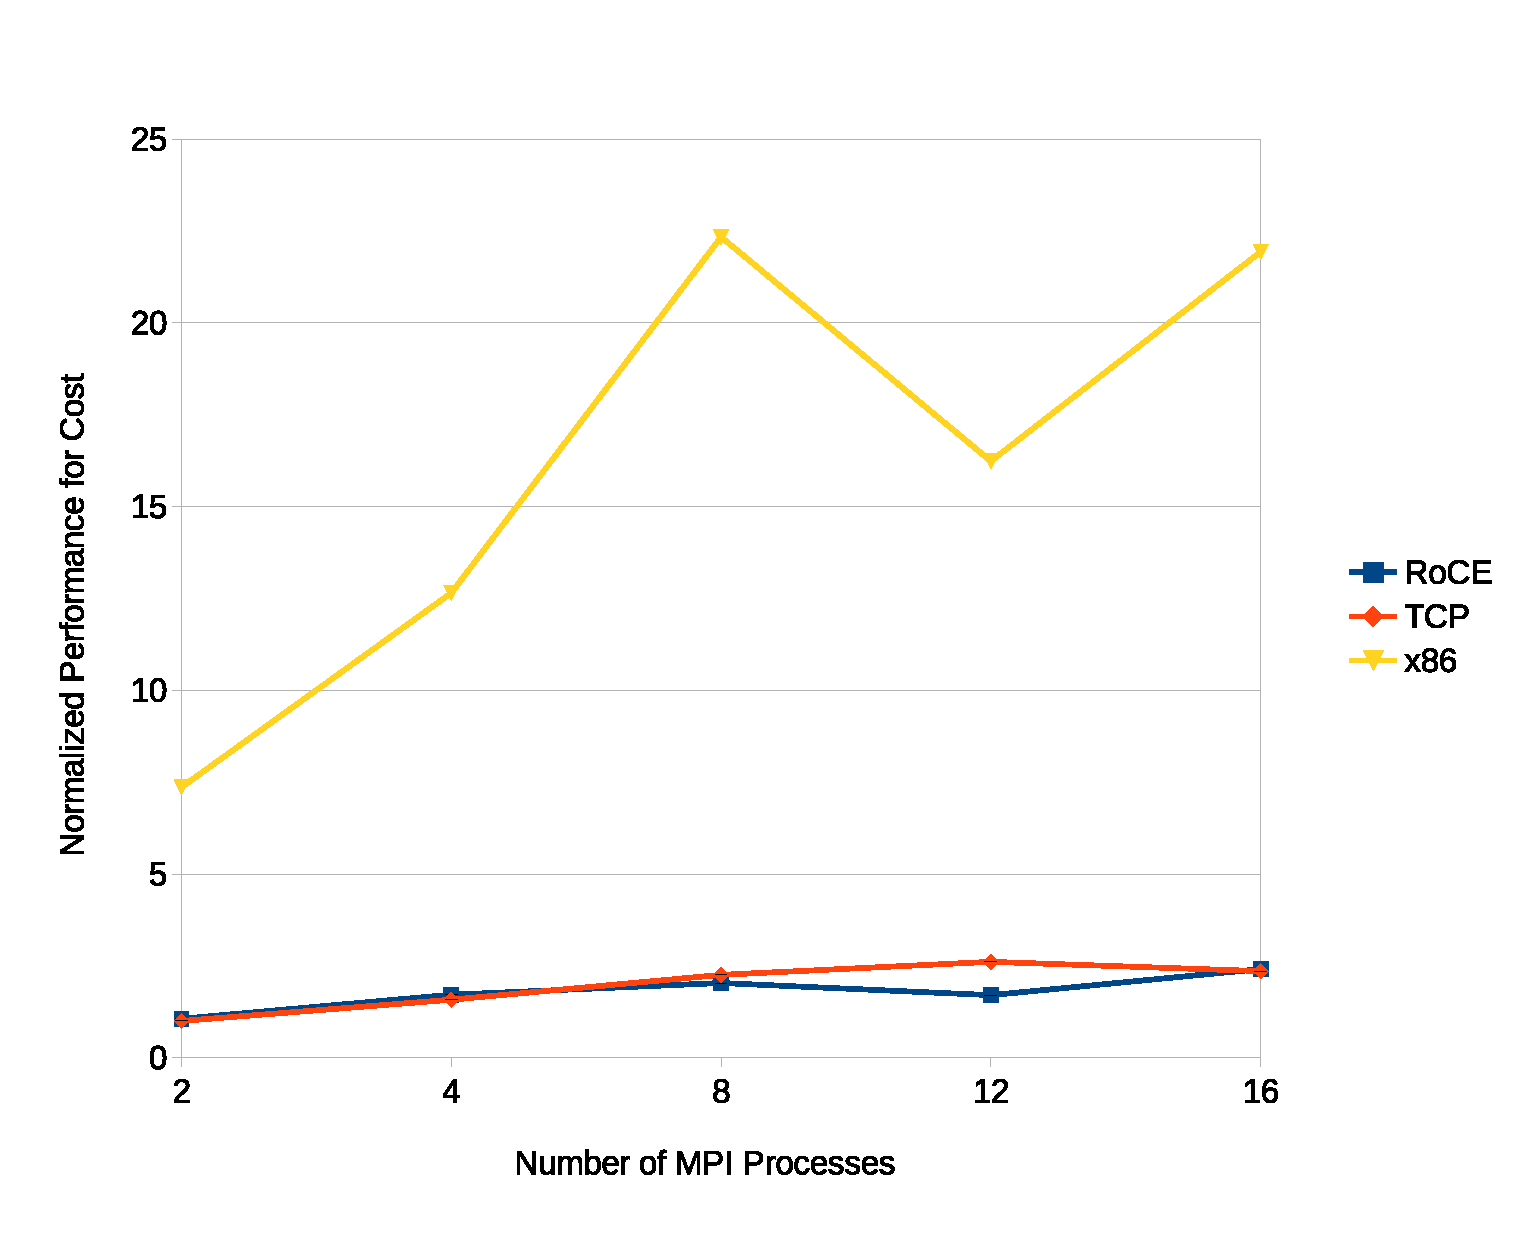
\includegraphics[width=0.75\textwidth]{disksim_costperf}
\caption{Normalized Performance for Cost for \textsc{disksim} Model}
\label{disksim-costperf}
\end{figure}

\begin{figure}
\centering
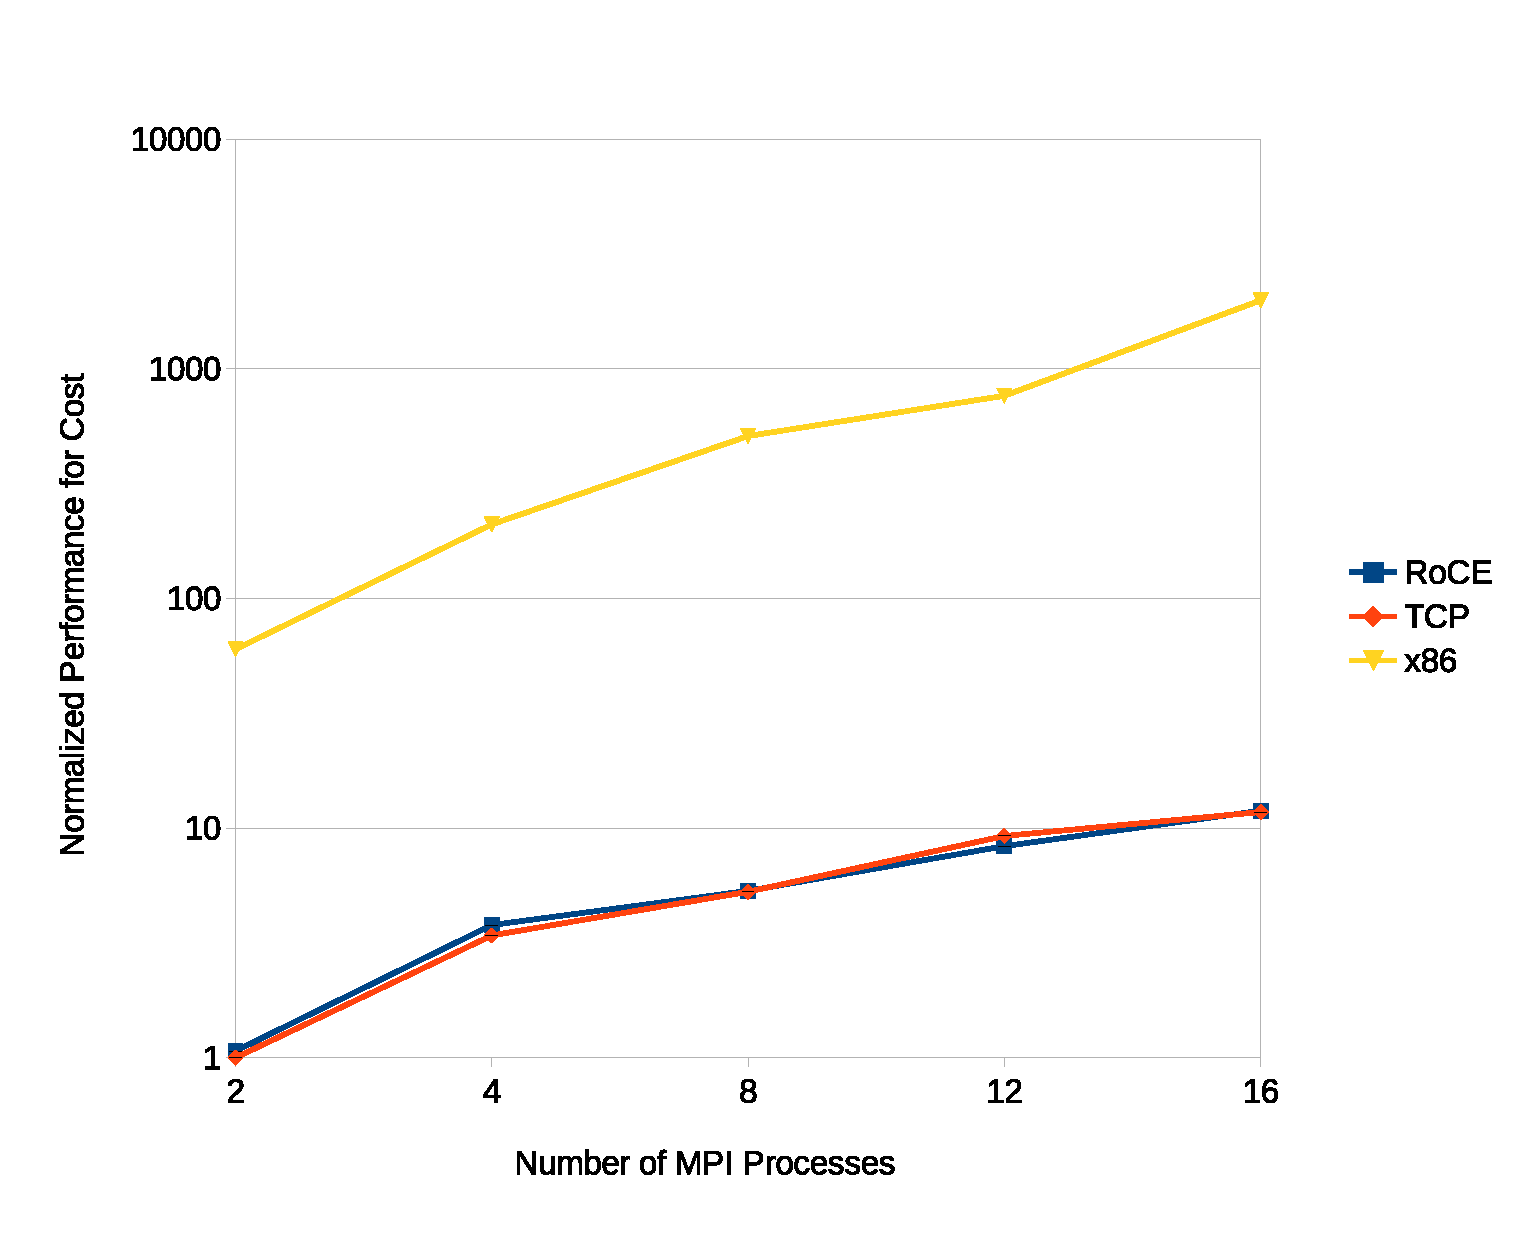
\includegraphics[width=0.75\textwidth]{raid_costperf}
\caption{Normalized Performance for Cost for \textsc{raid} Model}
\label{raid-costperf}
\end{figure}

\begin{figure}
\centering
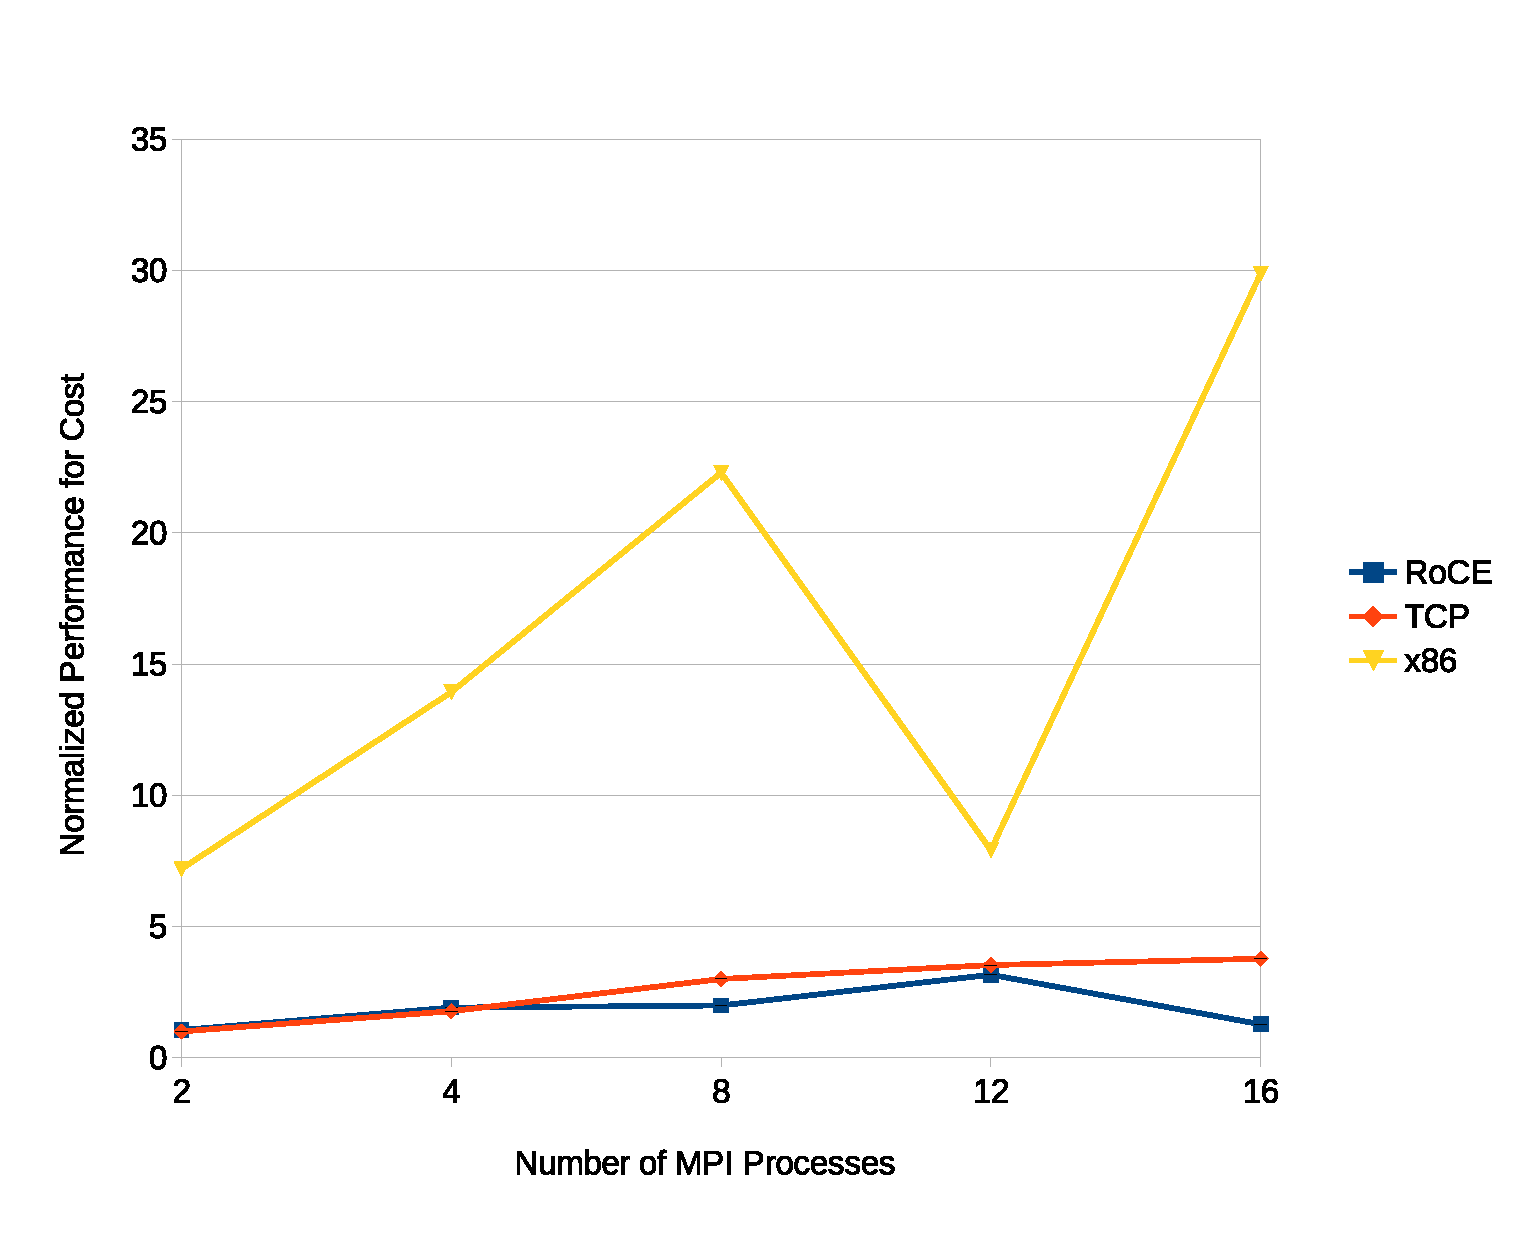
\includegraphics[width=0.75\textwidth]{wifi_costperf}
\caption{Normalized Performance for Cost for \textsc{wifi} Model}
\label{wifi-costperf}
\end{figure}

In all cases, the x86 cluster exhibits superior performance-for-cost compared to
our ARM cluster. \textbf{Figure \ref{costperf}} shows the worst-case
performance-for-cost comparison for the x86 cluster in comparison to the ARM
cluster. The x86 cluster is at least 3 times more cost-efficient than the ARM
cluster for PDES.

\begin{figure}
\centering
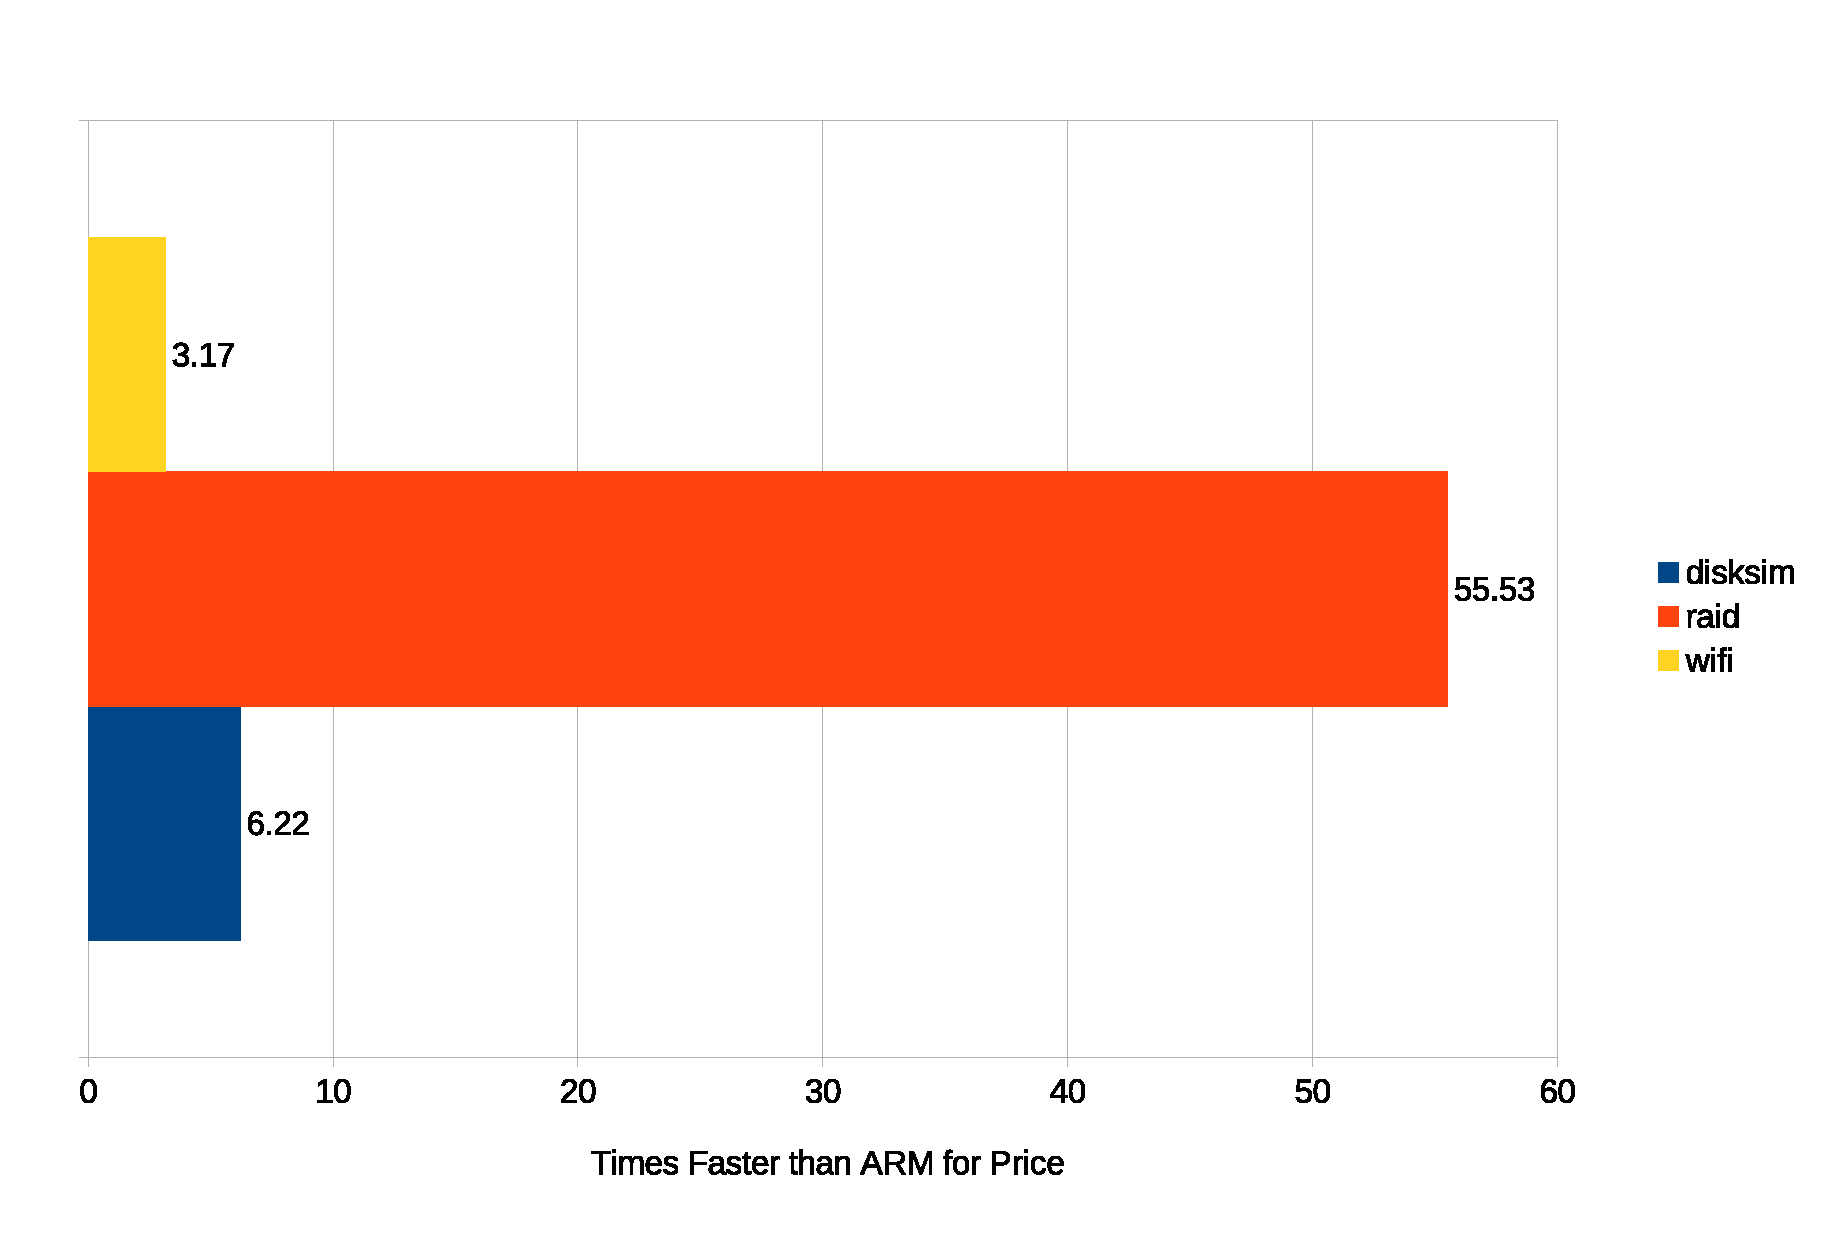
\includegraphics[width=\textwidth]{costperf}
\caption{Performance for Cost of x86 Cluster Compared to ARM Cluster}
\label{costperf}
\end{figure}

\textbf{Figure \ref{costperf-summary}} shows the performance-for-cost comparison
to baseline for each model. This compares how performance scales for each model
and each cluster as more MPI processes are added. We observe that the
\verb;raid; model scales more efficiently than the other models we tested. From
this, we learn that PDES performance depends significantly on simulation
modeling techniques as well as network performance, and the cost of adding nodes
to a cluster is more likely to be justified if one uses models similar to the
ROSS \verb;raid; model than if one uses models similar to either \verb;disksim;
or \verb;wifi;. Additionally, the x86 cluster takes advantage of parallelism
more efficiently than the ARM cluster for all three models.

\begin{figure}
\centering
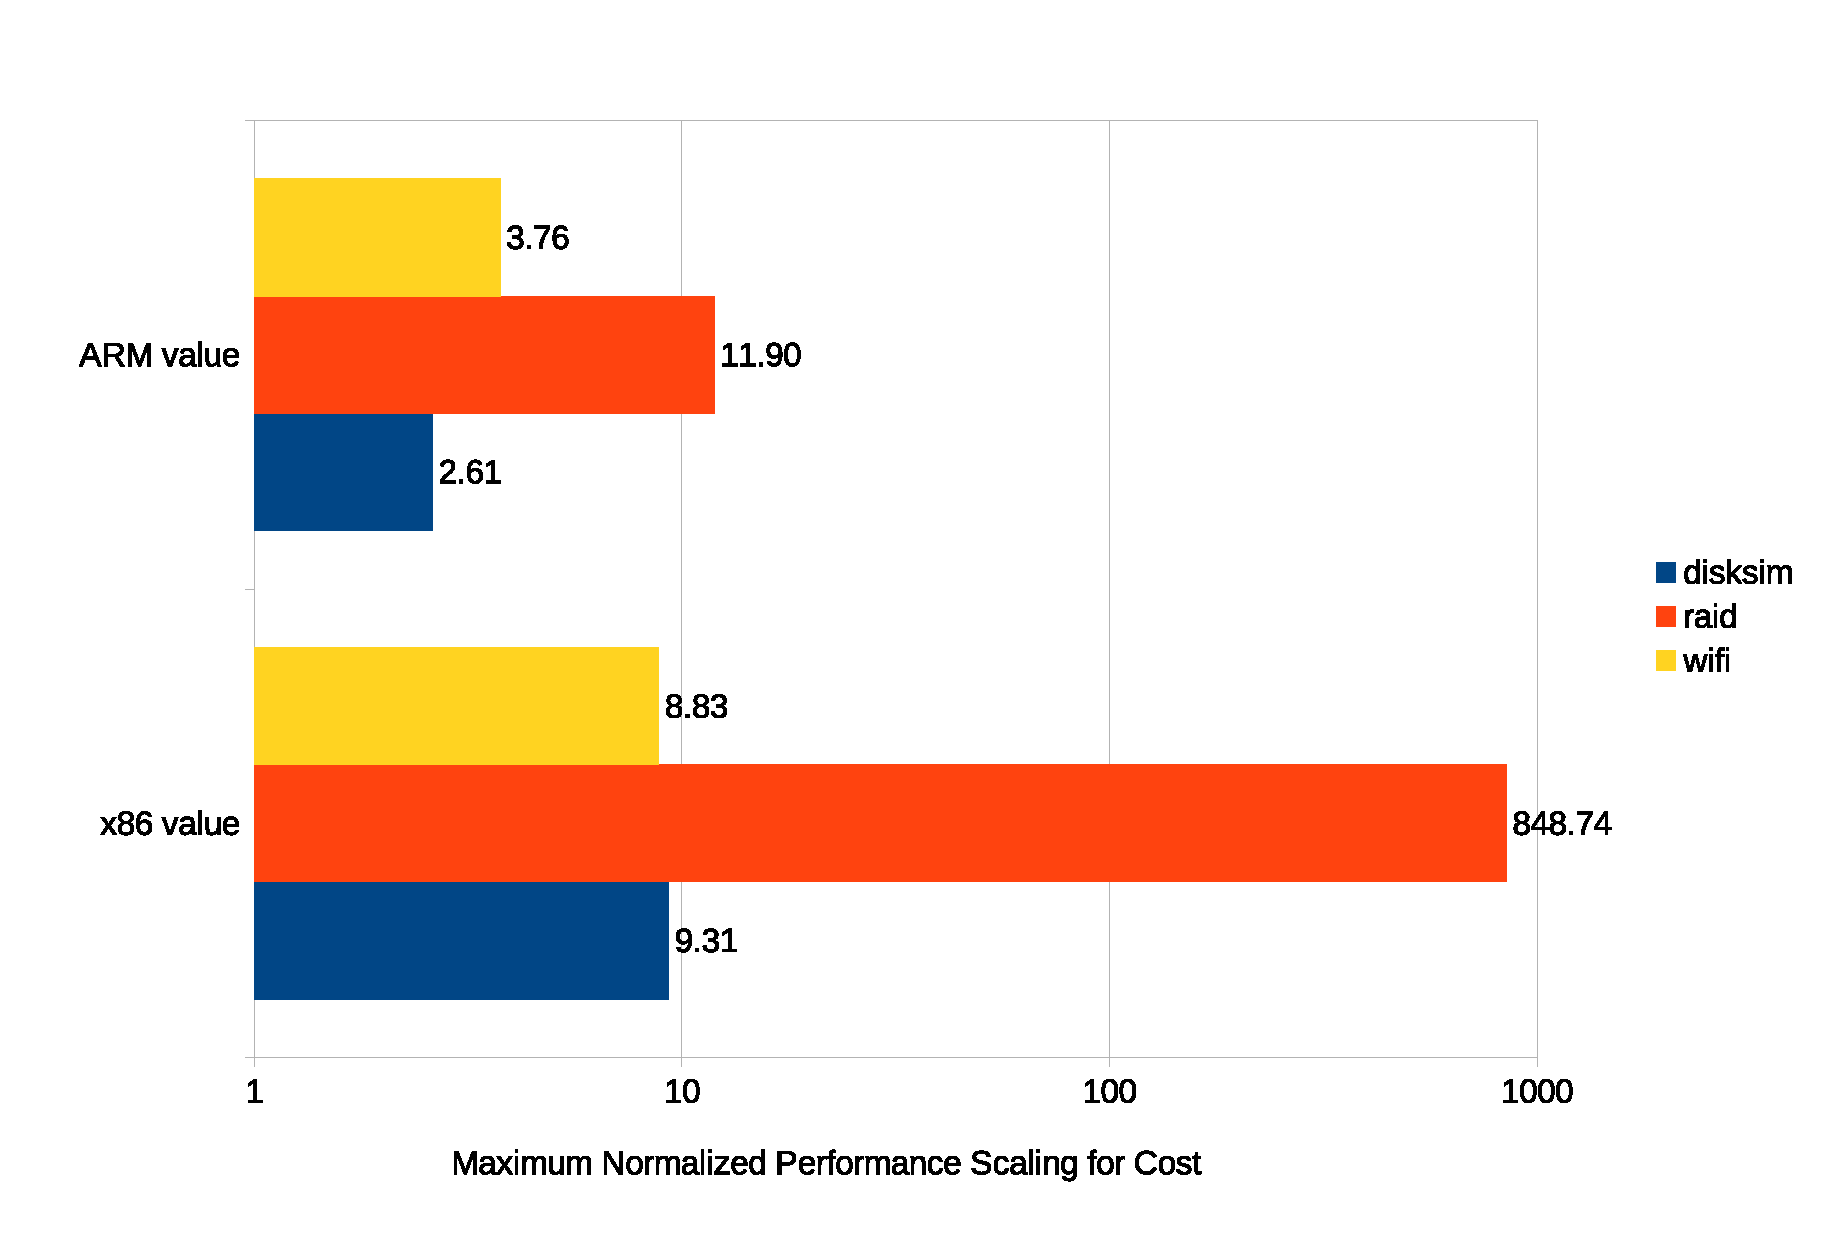
\includegraphics[width=\textwidth]{costperf_summary}
\caption{Scaling of Model Performance for Cost with Parallelism on Each Platform}
\label{costperf-summary}
\end{figure}

\section{\textbf{Conclusions}}

The software RoCE transport increases ROSS performance by a consistent 5\% to
11\% over the TCP/IP transport when no more than one MPI process is allocated
per compute node for our cluster. With more than one MPI process per node, RoCE
performance is less consistent. Execution stalls occasionally as rollbacks
cascade, doubling or tripling execution time, perhaps once per ten runs. A
configuration of three processes per node is particularly susceptible to this
effect, leading us to conclude that disparity betweeen remote and local
communication latency may be the cause of this problem.

In terms of both raw computing power for price and PDES performance for price,
our x86 cluster is far more efficient than our ARM cluster. However, the The x86 cluster also
exhibits tendencies that appear to lead to better scaling with increased
parallelism than the ARM cluster.

\section{\textbf{Challenges in SoC-based HPC}}

In this section, a few architectural challenges are presented that,
collectively, represent a barrier to adoption of clusters built from mobile
SoCs. Most of these issues are caused by valid design decisions on the part of
SoC vendors, considering their primary market. Possible solutions are also
discussed.

\subsection{\textbf{PoP Memory}}

In our search for inexpensive cluster nodes, we found that a drawback to mobile
SoCs is their limited main memory that is typically included in a Package on
Package (PoP) assembly, making it impossible for the end user to
upgrade. Although current mobile operating systems are parsimonious with memory,
the opposite is true for HPC and, in particular, optimistically synchronized
PDES. In our studies, we were limited to relatively small simulation model sizes
for our PDES tests because of memory constraints rather than execution time
constraints.

Although the amount of memory that vendors package on mobile SoCs is steadily
increasing, memory limitations prevent them from being a contender for
replacement of large cluster nodes. Regardless, the attractiveness of mobile SoC
nodes for a small-scale cluster is undeniable.

Including memory expansion slots on a mobile SoC is not currently feasible
because of package size constraints. However, vendors could offer multiple
versions of their chips with identical processors but different amounts of main
memory.

\subsection{\textbf{I/O Limitations}}

The lack of Peripheral Component Interconnect (PCI) support in the Exynos line
of SoCs means that all ethernet communications must be routed through a USB
interface. Although we saw that USB 3 reduces latency dramatically when compared
to USB 2, both incur significant latency penalties when compared to a PCI or PCI
Express (PCIe) network interface.

NVIDIA's Tegra 2 and Tegra 3 SoCs support PCIe, which provides access to a
relatively low-latency networking interface in a mobile platform
\cite{rajovic-13}. The Tegra 4 does not support PCIe \cite{arstch-tegra},
illustrating the lack of demand for high speed I/O in mobile devices.

The Linux system images for the ODROID boards are hosted on small flash memory
devices: microSD cards for the ODROID-XU and eMMC cards for the ODROID-U2. This
fact alone eliminates the possibility of any ``disk-intensive'' programs from
running well on our cluster.

Again, the Tegra 2 and 3 include support for SATA disks, but the Tegra 4 does
not \cite{arstch-tegra}.

\subsection{\textbf{Memory Errors}}

High Performance Computing platforms typically use Error Correcting Code (ECC)
main memory in order to avoid data corruption that could taint scientific
results. Commodity processors rarely include support for ECC memory because such
errors can be tolerated in a desktop or mobile computing environment. Because
Low Power Double Data Rate (LPDDR) memory does not support ECC, there is no way
to measure the incidence of memory errors in our own cluster; further, there is
no way

Although conventional wisdom suggests that memory errors are rare in practice, a
recent study by Schroeder et al. \cite{schroeder-09} on ECC memory found that
8.2\% of all tested memory modules were affected by at least one error per
year. Additionally, the incidence of memory errors increased with memory module
density. This makes sense when one considers the possibility of charge sharing
in the memory modules. This implies that memory errors are even more likely in
an SoC environment where memory density is very high.

A significant step toward enabling mobile SoCs for deployment in HPC
applications would be to include ECC memory. Most current ECC implementations
can correct single-bit-per-word errors, which account for almost all memory
errors observed in Schroeder's study \cite{schroeder-09} and detect more severe
errors, ensuring that bit flips cannot affect computation results without the
user's knowledge.

\section{\textbf{Benefits of SoC-based HPC}}

This section discusses some of our discoveries about the benefits of SoC-based
clusters.

\subsection{\textbf{Commodity Pricing}}

Although the ARM cluster from this project falls short of a traditional x86
Beowulf cluster in terms of performance for price, the possibility of
constructing an inexpensive multi-node cluster may be attractive to some
researchers. This is the same economic force that drove the adoption of Beowulf
clusters in the first place: inexpensive commodity microprocessors intended for
workstations gradually became more attractive than expensive custom solutions
for small-scale High Performance Computing.

\subsection{\textbf{Small Form Factor}}

Traditional Beowulf clusters require physical space and infrastructure for power
and cooling that is not necessary for SoC-based clusters. In fact, a very large
cluster of ARM-based PCs can fit in the same physical space as a single
x86-based PC. Their power supplies are also much smaller than corresponding x86
power supplies. In fact, an advantage of the mobile SoC design is that the
entire board runs from a single external power rail. This is in contrast to most
x86 PCs, which require several different voltage supply rails from a power
supply. This fact opens possibilities for innovative packaging solutions for
SoC-based clusters, from large lattices to small fanless configurations.

\section{\textbf{Suggestions for Future Work}}

I have touted the ability to deploy custom operating systems in a cluster
environment as a benefit of SoC-based HPC. Creating a custom operating
system is a significant commitment toward a platform that is not yet proven to
scale well for PDES. However, new hardware features such as hardware
virtualization support and Large Physical Address Extension support reduce the
risk associated with such a project.

Similar work on a platform with support for lower latency networking through PCI
is likely to scale better with increases in number of MPI processes because the
disparity between local and remote latency will be less pronounced for each
node.

Comparison of the power dissipated by our ARM cluster and the power dissipated
by our x86 cluster would be interesting, especially as it pertains to discussion
about scaling costs. Because an ARM-based cluster would probably require more
nodes than an x86 cluster to achieve similar computing performance, it is not
clear which architecture would actually be more efficient at a large scale.

\newpage
%%\bibliographystyle{abbrv} 
\bibliographystyle{IEEEtran} 
\bibliography{refs}

\end{document}
